\documentclass[a4paper,12pt]{extarticle}
\usepackage{geometry}
\usepackage[T1]{fontenc}
\usepackage[utf8]{inputenc}
\usepackage[english,russian]{babel}
\usepackage{enumitem}
\usepackage{amsmath}
\usepackage{amsthm}
\usepackage{amssymb}
\usepackage{fancyhdr}
\usepackage{setspace}
\usepackage{graphicx}
\usepackage{colortbl}
\usepackage{tikz}
\usepackage{pgf}
\usepackage{subcaption}
\usepackage{listings}
\usepackage{indentfirst}
\usepackage[
backend=bibtex,
style=numeric,
maxbibnames=99
]{biblatex}
\addbibresource{refs.bib}
\usepackage[colorlinks,citecolor=blue,linkcolor=blue,bookmarks=false,hypertexnames=true, urlcolor=blue]{hyperref} 
\usepackage{indentfirst}
\usepackage{mathtools}
\usepackage{booktabs}
\usepackage[flushleft]{threeparttable}
\usepackage{tablefootnote}

\usepackage{chngcntr} % нумерация графиков и таблиц по секциям
\counterwithin{table}{section}
\counterwithin{figure}{section}

\graphicspath{{graphics/}}%путь к рисункам

\makeatletter
% \renewcommand{\@biblabel}[1]{#1.} % Заменяем библиографию с квадратных скобок на точку:
\makeatother

\geometry{left=2.5cm}% левое поле
\geometry{right=1.0cm}% правое поле
\geometry{top=2.0cm}% верхнее поле
\geometry{bottom=2.0cm}% нижнее поле
\setlength{\parindent}{1.25cm}
\renewcommand{\baselinestretch}{1.5} % междустрочный интервал


\newcommand{\bibref}[3]{\hyperlink{#1}{#2 (#3)}} % biblabel, authors, year
\addto\captionsrussian{\def\refname{Список литературы (или источников)}} 

\renewcommand{\theenumi}{\arabic{enumi}}% Меняем везде перечисления на цифра.цифра
\renewcommand{\labelenumi}{\arabic{enumi}}% Меняем везде перечисления на цифра.цифра
\renewcommand{\theenumii}{.\arabic{enumii}}% Меняем везде перечисления на цифра.цифра
\renewcommand{\labelenumii}{\arabic{enumi}.\arabic{enumii}.}% Меняем везде перечисления на цифра.цифра
\renewcommand{\theenumiii}{.\arabic{enumiii}}% Меняем везде перечисления на цифра.цифра
\renewcommand{\labelenumiii}{\arabic{enumi}.\arabic{enumii}.\arabic{enumiii}.}% Меняем везде перечисления на цифра.цифра

\DeclareFieldFormat{labelnumberwidth}{#1\adddot}

\begin{document}
\begin{titlepage}
\newpage

{\setstretch{1.0}
\begin{center}
ПРАВИТЕЛЬСТВО РОССИЙСКОЙ ФЕДЕРАЦИИ\\
ФГАОУ ВО НАЦИОНАЛЬНЫЙ ИССЛЕДОВАТЕЛЬСКИЙ УНИВЕРСИТЕТ\\
«ВЫСШАЯ ШКОЛА ЭКОНОМИКИ»
\\
\bigskip
Факультет компьютерных наук\\
Образовательная программа «Прикладная математика и информатика»
\end{center}
}

\vspace{7em}

\begin{center}
{\bf ВЫПУСКНАЯ КВАЛИФИКАЦИОННАЯ РАБОТА}\\
%Выберите какой у вас проект
{\bf Исследовательский проект на тему:}\\
%{\bf Программный проект на тему:}\\
%{\bf Отчет о командном программном проекте на тему:}\\
{\bf Сжатие словарей для нейросетевого анализа исходных кодов программ}\\
\end{center}

\vspace{2em}

{\bf Выполнил студент: \vspace{2mm}}

{\setstretch{1.1}
\begin{tabular}{l@{\hskip 1.5cm}l}
группы \#БПМИ171, 4 курса & Гусев Андрей Алексеевич 
\end{tabular}}

% Обычно у вас есть один научный руководитель, и это человек, с которым вы работаете над проектом. Иногда по формальным причинам у вас будет руководитель (штатный сотрудник Вышки) и соруководитель (тот, с кем вы работаете), — об этом вам сообщит учебный офис (в случае с ВКР) или ЦППРиП (в случае с курсовым проектом). Также, если кто-то дополнительно вам помогал, то его можно указать как консультанта. 

%ваш официальный научник (из ВШЭ)
\vspace{1em}
{\bf Принял руководитель ВКР: \vspace{2mm}}

{\setstretch{1.1}
\begin{tabular}{l}
Чиркова Надежда Александровна\\
Научный сотрудник\\
Факультет компьютерных наук НИУ ВШЭ 
\end{tabular}}

% со-руководитель (если есть)
%\vspace{1em}
%{\bf Соруководитель: \vspace{2mm}}%это ваш официальный научник

%{\setstretch{1.1}
%\begin{tabular}{l}
%Петрова Надежда Александровна\\
%Инженер-исследователь\\
%ОАО Компания "Нейросети и деревья" 
%\end{tabular}}

% консультант (если есть)
%\vspace{1em}
%{\bf Консультант: \vspace{2mm}}%это ваш официальный научник

%{\setstretch{1.1}
%\begin{tabular}{l}
%Иванова Надежда Александровна\\
%Инженер-исследователь\\
%ОАО Компания "Нейросети и деревья" 
%\end{tabular}}

\vspace{\fill}

\begin{center}
Москва 2024
\end{center}

\end{titlepage}% это титульный лист - выберите подходящий вам из имеющихся в проекте вариантов (kr - курсовая работа у 3 курса, vkr - выпускная квалификационная работа у 4 курса)
\newpage
\setcounter{page}{2}

{
	\hypersetup{linkcolor=black}
	\tableofcontents
}

\newpage

\newpage
\section*{Аннотация}   % this is how to use russian
Выпускная квалификационная работа посвящена разработке эффективного и простого в использовании приложения, которое позволит пользователям легко и быстро подбирать категорию товара для маркетплейса по его фотографии, а также составлять к нему SEO-описание. В работе проведен анализ существующих решений, рассмотрены различные архитектуры нейронных сетей, описаны задачи классификации и создания подписей к изображениям, разработаны решения для реализации моделей нейронной сети для SEO-оптимизации карточки товара, учитывающие специфику данных. Особое внимание уделено использованным метрикам и методам сбора данных. Результатом работы является разработанный сервис, в основе которого реализована нейронная сеть, способная классифицировать товары на маркетплейсе на основе их фотографий и генерировать соответствующие к ним описания. Дальнейшие исследования в этой области могут включать улучшения качества результатов, а также расширение функциональности за счет генерации описания с помощью ключевых слов.

\addcontentsline{toc}{section}{Аннотация}

\newpage
\section*{Abstract}   % this is how to use russian
The final qualification work is devoted to the development of an effective and easy-to-use application that will allow users to easily and quickly select a product category for a marketplace based on its photo, as well as create an SEO description for it. The paper analyzes existing solutions, examines various architectures of neural networks, describes the tasks of classifying and creating captions to images, and develops solutions for implementing neural network models for SEO optimization of product cards, taking into account the specifics of the data. Special attention is paid to the metrics and data collection methods used. The result of the work is a developed service based on a neural network capable of classifying products on the marketplace based on their photos and generating descriptions corresponding to them. Further research in this area may include improvements in the quality of results, as well as expanding functionality by generating a description using keywords.

\newpage
\section*{Ключевые слова}   % this is how to use russian

\textbf{Маркетплейс (от англ. marketplace; электронная торговая площадка)} — платформа электронной коммерции, интернет-магазин электронной торговли, предоставляющий информацию о продукте или услуге третьих лиц.

\textbf{SEO-оптимизация карточек товара} — это процесс улучшения информации о товаре на маркетплейсе, чтобы она была более привлекательной и доступной для поисковых систем и пользователей. Цель состоит в том, чтобы повысить видимость товара в результатах поиска, привлечь больше потенциальных покупателей и увеличить конверсию.

\textbf{Искусственный интеллект (ИИ) (от англ. Artificial Intelligence, AI)} — свойство интеллектуальных компьютерных систем, обладающих возможностями выполнять творческие задачи, которые считаются прерогативой человека \cite{aiwebsite}.

\textbf{Машинное обучение (от англ. Machine Learning, ML)} — область искусственного интеллекта, изучающий различные способы построения обучающихся алгоритмов. Среди множества парадигм и подходов в машинном обучении выделяются нейронные сети \cite{mlwebsite}. 

\textbf{Компьютерное зрение (от англ. Computer Vision, CV)} — область искусственного интеллекта, которое занимается задачами, связанными с анализом изображений и видео \cite{cvwebsite}.

\textbf{Обработка естественного языка (от англ. Natural Language Processing, NLP)} — это направление в машинном обучении, посвящённое распознаванию, генерации и обработке устной и письменной человеческой речи \cite{nlpwebsite}.

\textbf{Нейронная сеть (от англ. Neural Network)} — математическая модель, а также ее программное или аппаратное воплощение, построенная по принципу организации и функционирования биологических нейронных сетей, используемая для решения задач ИИ \cite{neuralwebsite}.

Сокращения названий архитектур нейронных сетей:
\begin{itemize}
	\item сверточная нейронная сеть (от англ. Convolutional Neural Network, CNN);
	\item рекуррентная нейронная сеть (от англ. Recurrent Neural Network, RNN);
	\item рекуррентная нейронная сеть с долгой краткосрочной памятью (от англ. Long Short-Term Memory, LSTM);
	\item управляемый рекуррентный блок (от англ. Gated Recurrent Unit, GRU);
	\item генеративный предварительно обученный трансформер, (от англ. Generative Pre-trained Transformer, GPT).
\end{itemize}

\newpage
\section*{Введение}   % this is how to use russian
В современном мире маркетплейсы стали неотъемлемой частью электронной коммерции, предоставляя платформы для продажи товаров и услуг различным производителям и ритейлерам.
В 2023 году маркетплейсы оставались основной движущей силой российской онлайн-торговли. Объем расходов на этих платформах вырос в 1.5 раза по сравнению с предыдущим годом, что говорит о продолжающемся росте интереса потребителей к онлайн-покупкам. Этому способствуют общерыночные факторы: развитие альтернативных каналов поставок продукции вместо ушедших брендов, улучшение условий доставки, повышение удобства использования платформ и расширение сети пунктов выдачи.

Согласно исследованиям «Tinkoff Ecommerce»\cite{tinkoffresearch}, за год количество транзакций на маркетплейсах увеличилось на 63\% (см. рисунок ~\ref{fig:marketplaces-purchases-increased}). Наибольший рост числа покупок показали платформы «Мегамаркет» (рост в 4.3 раза), «Wildberries» (увеличение в 2 раза) и «Ozon» (рост в 1.6 раза).

\begin{figure}[hbtp]
	\centering
	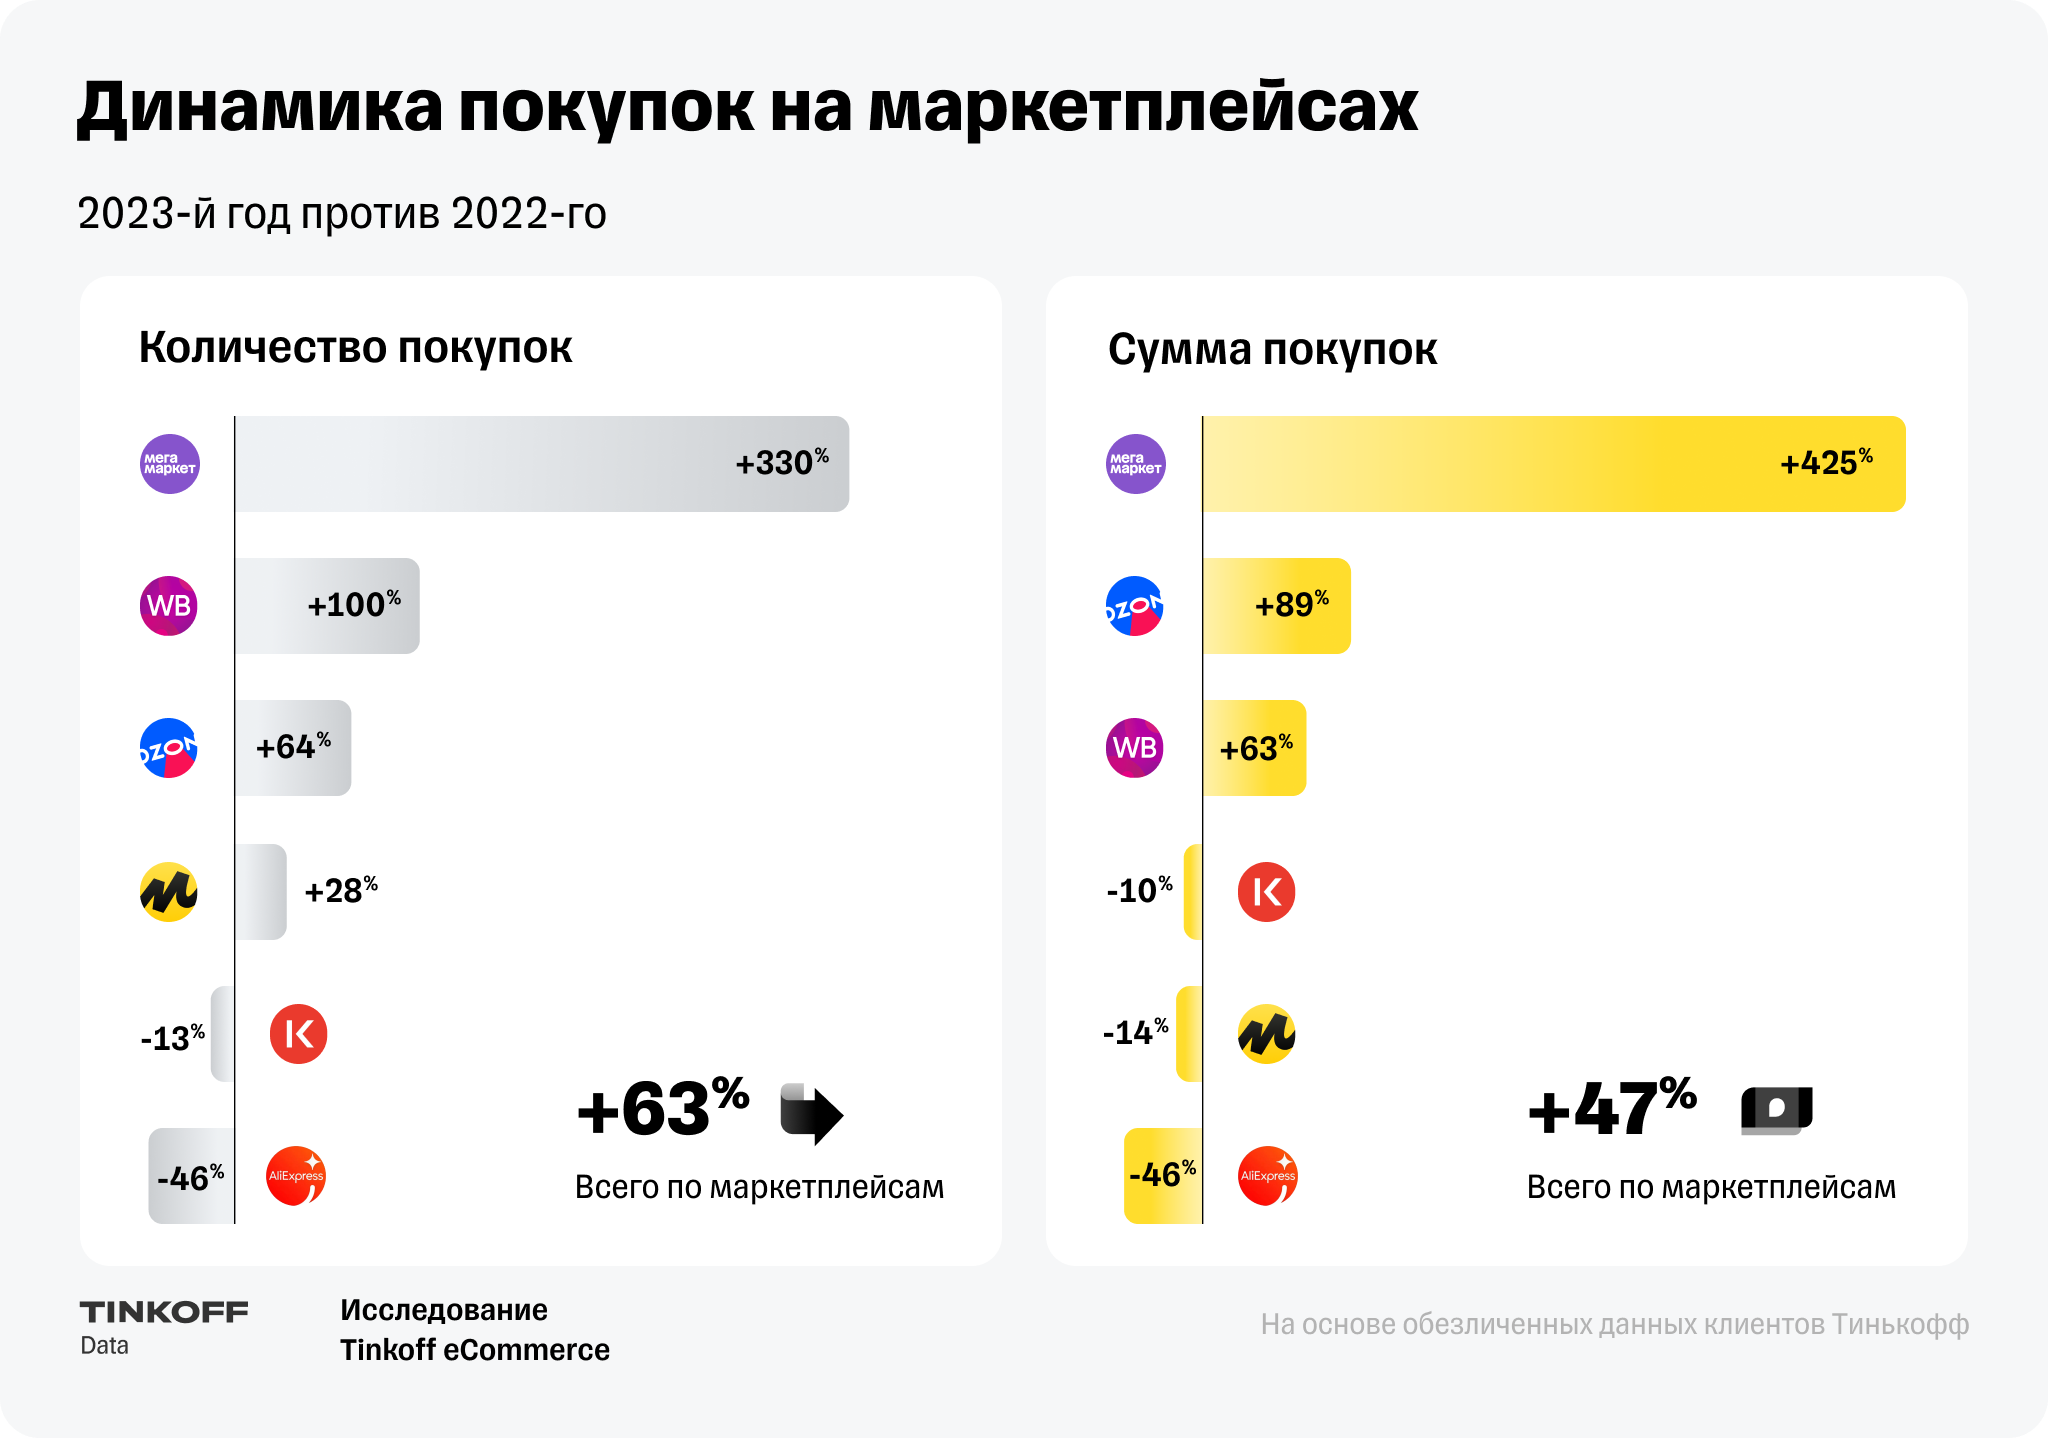
\includegraphics[scale=0.3]{marketplaces-purchases-increased.png}
	\caption{Динамика покупок на маркетплейсах в регионах \cite{tinkoffresearch}.}
	\label{fig:marketplaces-purchases-increased}
\end{figure} 

В российских регионах наблюдается рост популярности маркетплейсов. В 2023 году жители российских городов стали значительно активнее совершать покупки на онлайн-платформах, что привело к увеличению как количества транзакций, так и их общей суммы (см. рисунок ~\ref{fig:marketplaces-regions}). Особенно заметен рост числа транзакций в таких городах, как Омск (+91\%), Красноярск (+88\%), Новосибирск (+79\%), Челябинск (+79\%) и Волгоград (+75\%). В Москве прирост числа транзакций составил всего 41\%. Увеличение интереса к маркетплейсам в регионах связано с расширением географического охвата платформ, развитием сетей пунктов выдачи заказов, а также улучшением условий доставки и логистики.

\begin{figure}[hbtp]
	\centering
	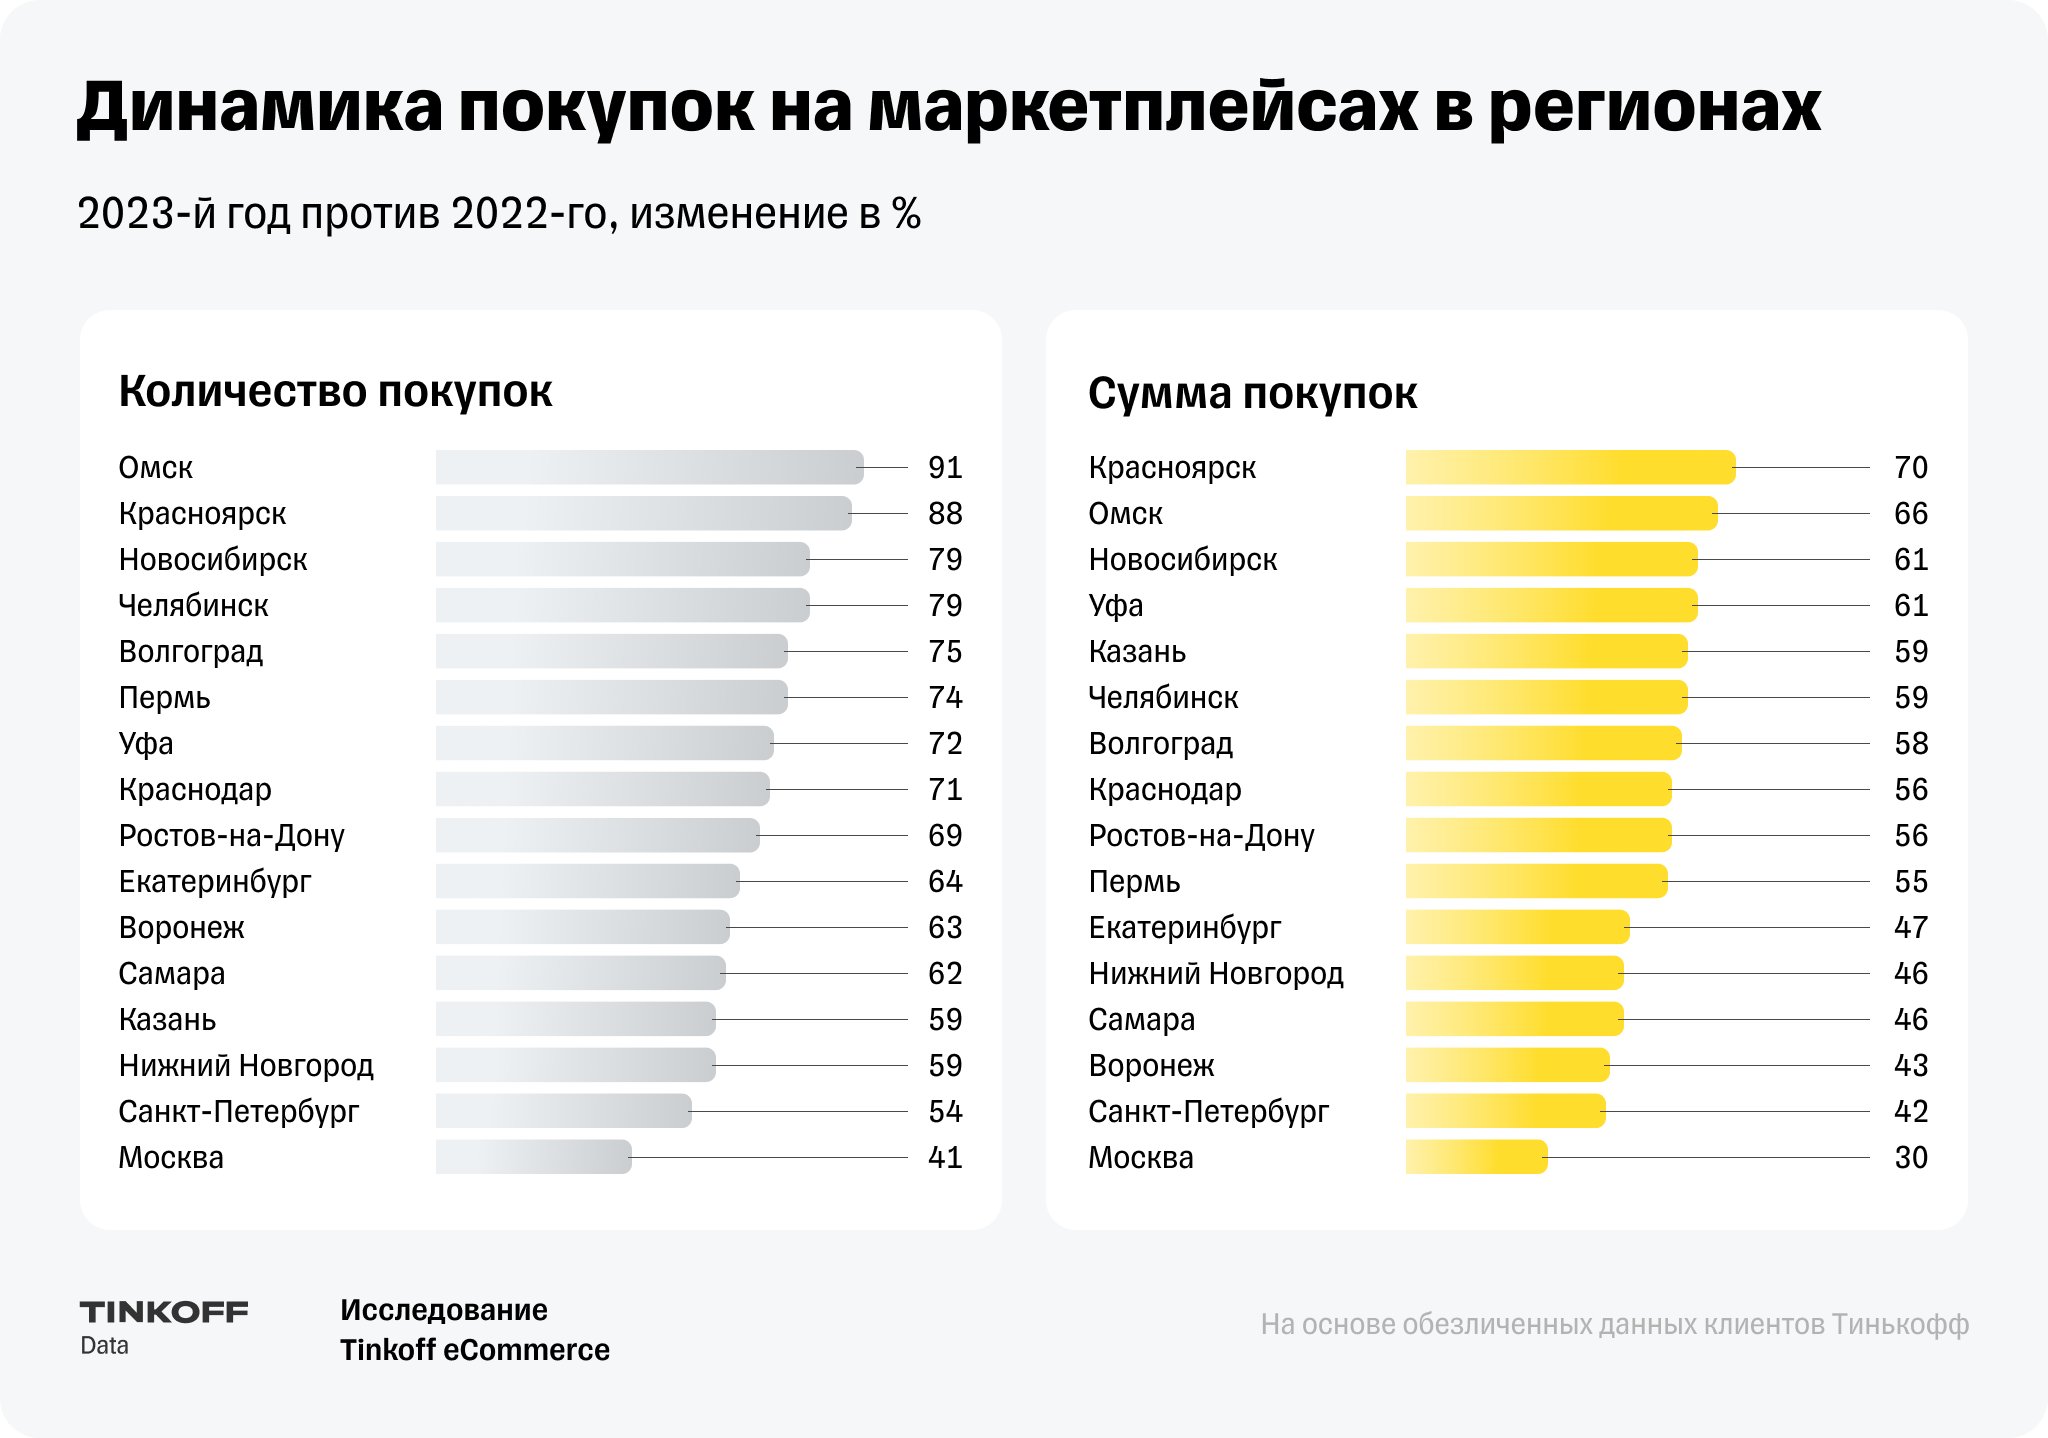
\includegraphics[scale=0.3]{marketplaces-regions.png}
	\caption{Динамика покупок на маркетплейсах в регионах \cite{tinkoffresearch}.}
	\label{fig:marketplaces-regions}
\end{figure}  

Вместе с тем выросло количество селлеров на 8\%. Рынок приобретает большую зрелость: менее опытные продавцы уступают место более профессиональным. Эти предприниматели ведут бизнес уверенно, укрепляют свои позиции на площадках и одновременно торгуют на нескольких платформах. За год число селлеров, работающих на двух и более маркетплейсах, выросло на 17\%. Наиболее привлекательной платформой для начала бизнеса стала «Wildberries»: в конце 2023 года ее выбирали в качестве первой площадки 63\% продавцов (см. рисунок ~\ref{fig:marketplaces-top}).

\begin{figure}[hbtp]
	\centering
	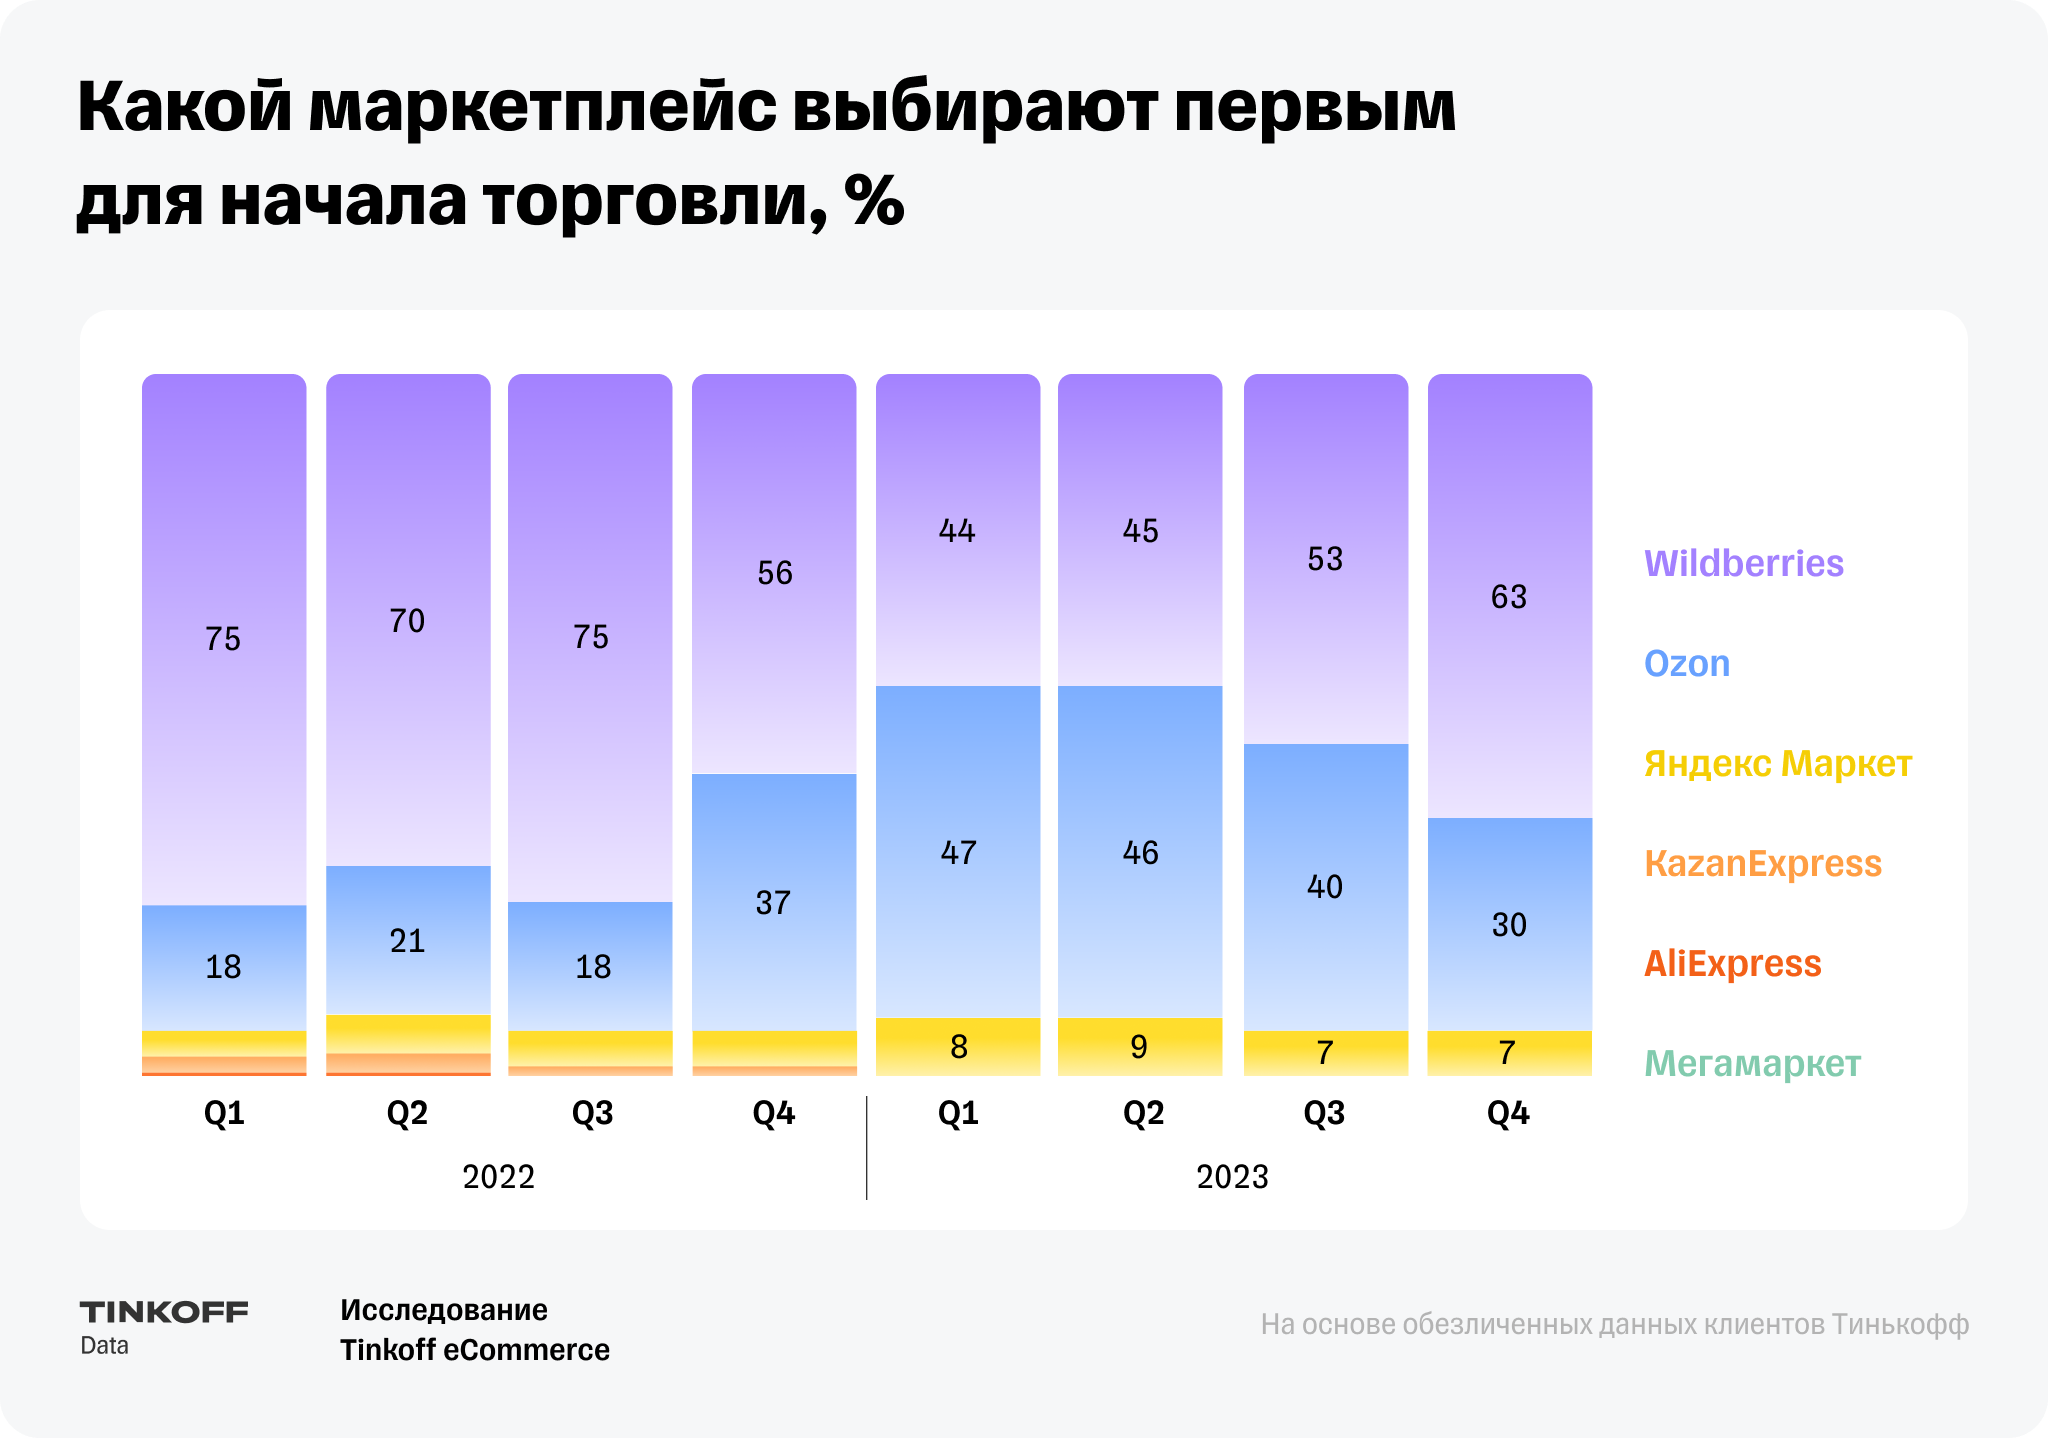
\includegraphics[scale=0.3]{marketplaces-top.png}
	\caption{Популярность маркетплейсов за 2023 год \cite{tinkoffresearch}.}
	\label{fig:marketplaces-top}
\end{figure} 

С увеличением конкуренции продавцы все чаще обращаются к системам, которые могут помочь им в продажах, а также автоматизировать процесс работы. Одним из ключевых факторов успешной продажи становится эффективная SEO-оптимизация карточек товаров. Подбор наиболее подходящей категории и создание продаваемого описания, содержащего ключевые слова, позволяет улучшить видимость товаров в результатах поиска как на самом маркетплейсе, так и в поисковых системах, что напрямую влияет на увеличение продаж.

На данный момент существуют несколько сервисов (например, TurboTextPro, Gerwin, CopyMonkey, подробнее можно ознакомиться в пункте \ref{exists}), позволяющих сгенерировать описание товаров по характеристикам, ключевым словам или фотографии. Однако, качество сгенерированных описаний не всегда позволяют использовать их в системах автономного управления. В настоящее время российский рынок не предлагает специальных технологий и решений для подбора наиболее подходящей категории товара на маркетплейсе. Таким образом, задача создания качественного инструмента для эффективной SEO-оптимизации карточек товаров является актуальной. 

\addcontentsline{toc}{section}{Введение}

\newpage
\section{Цель и задачи работы}

Цель данной работы — разработать сервис, в основе которого будет реализована модель нейронной сети, способная классифицировать товары на маркетплейсе на основе их фотографий и генерировать соответствующие к ним описания.

Для достижения поставленной цели необходимо решить следующие задачи:
\begin{itemize}
	\item подготовить набор данных, содержащий изображения товаров и соответствующие им категории и текстовые описания;
	\item провести исследование текущих решений, используемых для классификации изображений и генерации текста, и на основе этого исследования создать наиболее подходящую архитектуру модели для решения поставленной задачи;
	\item обучить спроектированную архитектуру на подготовленных данных, оптимизировать и настроить параметры модели для повышения её производительности и качества результатов, а затем оценить эффективность реализованной архитектуры;
	\item интегрировать модель в программное обеспечение.
\end{itemize}

\newpage
\section{Постановка задачи}

В соответствии с заданием на выпускную квалификационную работу необходимо разработать программное обеспечение, на вход которого подаются фотографии товара. Выходом являются наиболее подходящая категория товара для маркетплейса и его SEO-описание.

Допущения:
\begin{itemize}
	\item рассматривается только маркетплейс «Wildberries»;
	\item глубина подбора категории — второй уровень вложенности.
\end{itemize}

Постановка задачи в виде IDEF0-диаграммы представлена на рисунке \ref{fig:hse-idef0}. 

\begin{figure}[ht]
	\centering
	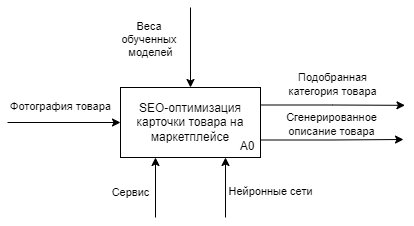
\includegraphics[scale=0.8]{hseidef0.png}
	\caption{Постановка задачи.}
	\label{fig:hse-idef0}
\end{figure}

Для достижения целей и задач проекта требуется решить задачу многоклассовой классификации изображений (от англ. multiclass image classification) для подбора наиболее подходящей категории по фотографии товара, а также решить задачу создания подписей к изображениям (от англ. image captioning). Для успешной реализации проекта необходимо выбрать подходящие модели и определить метрики, которые будут использоваться для оценки их эффективности.

\newpage
\section{Обзор существующих решений}\label{exists}

На данный момент существуют несколько сервисов, позволяющих сгенерировать описание товаров по характеристикам, ключевым словам или фотографии. Однако нет сервисов для подбора наиболее подходящей категории товара на маркетплейсе по фотографии. Для продавцов было бы крайне полезно иметь эти функциональности одновременно. Это значительно упростило бы процесс подготовки и публикации товаров, а также повысило эффективность и точность их работы.

\subsection{TurboText.Pro}

TurboText.Pro — это сервис, который создает описания по фотографии или характеристикам товара \cite{turbotextpro}. Во втором случае текст будет более качественным, так как ИИ генерирует описание на основе заданных параметров. Нейросеть создает три описания для одного товара, что позволяет выбрать лучший вариант и разместить его в карточке товара или использовать все варианты на разных платформах. Также можно заказать улучшение текста или SEO-оптимизацию для продвижения товара на «Wildberries» у опытных копирайтеров.

Преимущества данного сервисы:
\begin{itemize}
	\item высокая скорость генерации (1-2 секунды);
	\item развернутое описание товара;
	\item все функции доступны бесплатно;
	\item возможность сгенерировать описание товара по фотографии или характеристикам;
	\item возможность заказать SEO-оптимизацию описания товара.
\end{itemize}

Недостатки:
\begin{itemize}
	\item генерация только на русском языке;
	\item качество описания по фото ниже, чем описания по характеристикам товара;
	\item ограничение при генерации описания по характеристикам — от 30 символов.
\end{itemize}

На рисунках \ref{fig:turbotextpro} и \ref{fig:turbotext-photo} представлен интерфейс данного сервиса.

\begin{figure}[ht]
	\centering
	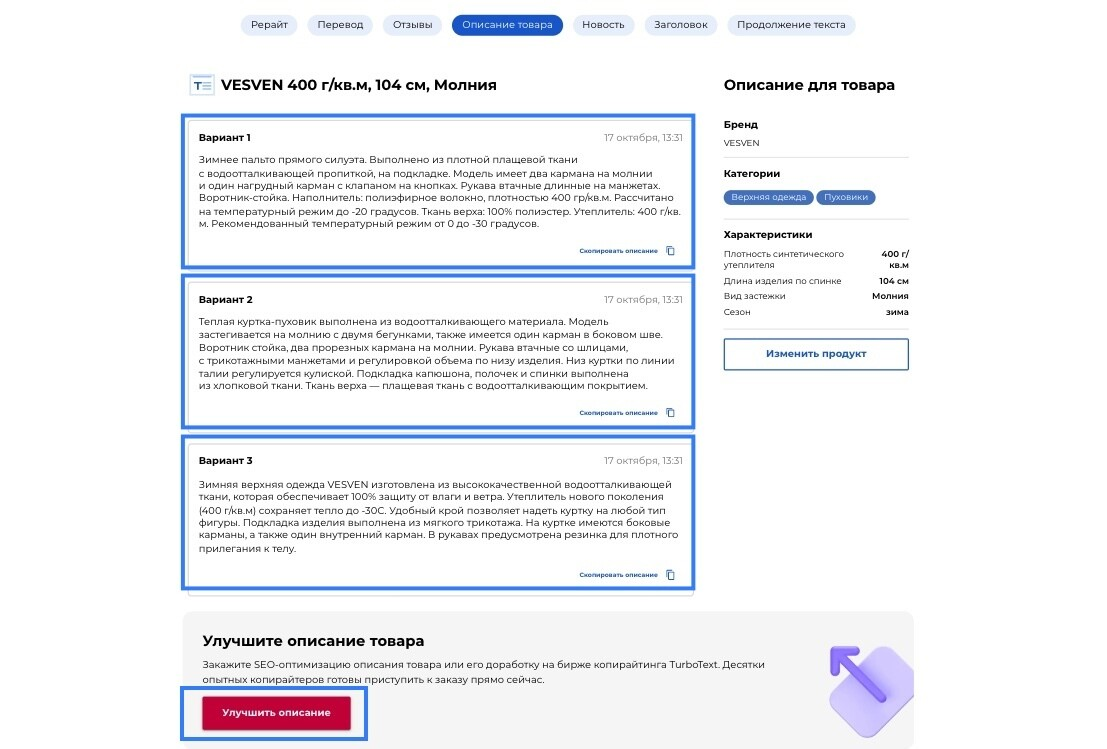
\includegraphics[scale=0.4]{turbotextpro.png}
	\caption{Генерация описание товара по характеристикам с помощью сервиса TurboText.Pro.}
	\label{fig:turbotextpro}
\end{figure}

\begin{figure}[ht]
	\centering
	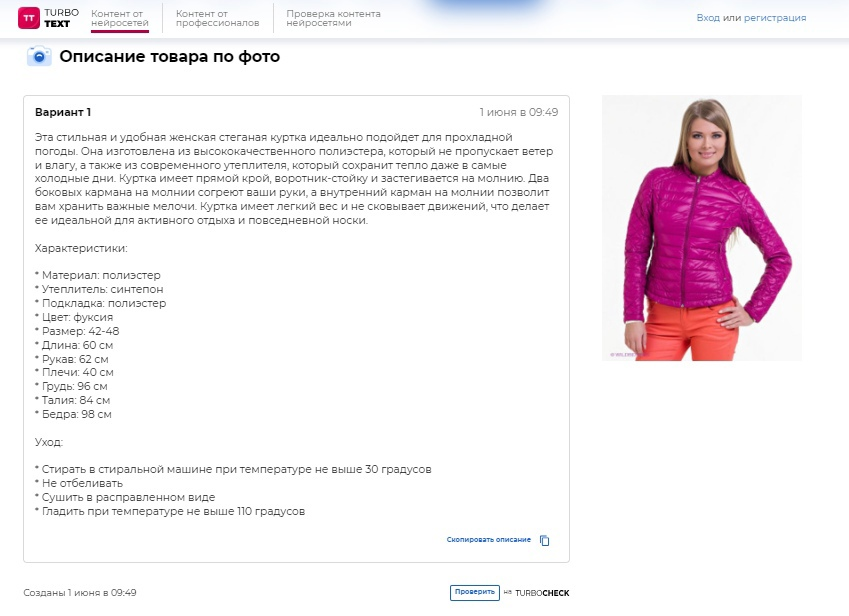
\includegraphics[scale=0.4]{turbotext-photo.png}
	\caption{Генерация описания товара по фотографии с помощью сервиса TurboText.Pro.}
	\label{fig:turbotext-photo}
\end{figure}

\newpage
\subsection{Gerwin}

Gerwin — создает описания для товара по ключевым словам \cite{gerwin}.

Преимущества данного сервисы:
\begin{itemize}
	\item высокая скорость генерации (1-2 секунды);
	\item есть варианты генерации на разных языках;
	\item разные описания к одному товару на выбор;
	\item можно протестировать сервис бесплатно по промокоду.
\end{itemize}

Недостатки:
\begin{itemize}
	\item ограничение по количеству ключевых слов — не больше 3-х;
	\item из-за ограничений исходных данных нельзя сделать более развернутое описание товара;
	\item нет возможности сгенерировать описание товара по фотографии;
	\item чтобы протестировать сервис бесплатно, нужно «добыть» промокод через Telegram-бота. Время ожидания — в течение 8 часов.
\end{itemize}

На рисунке \ref{fig:gerwin} представлен интерфейс данного сервиса.

\begin{figure}[ht]
	\centering
	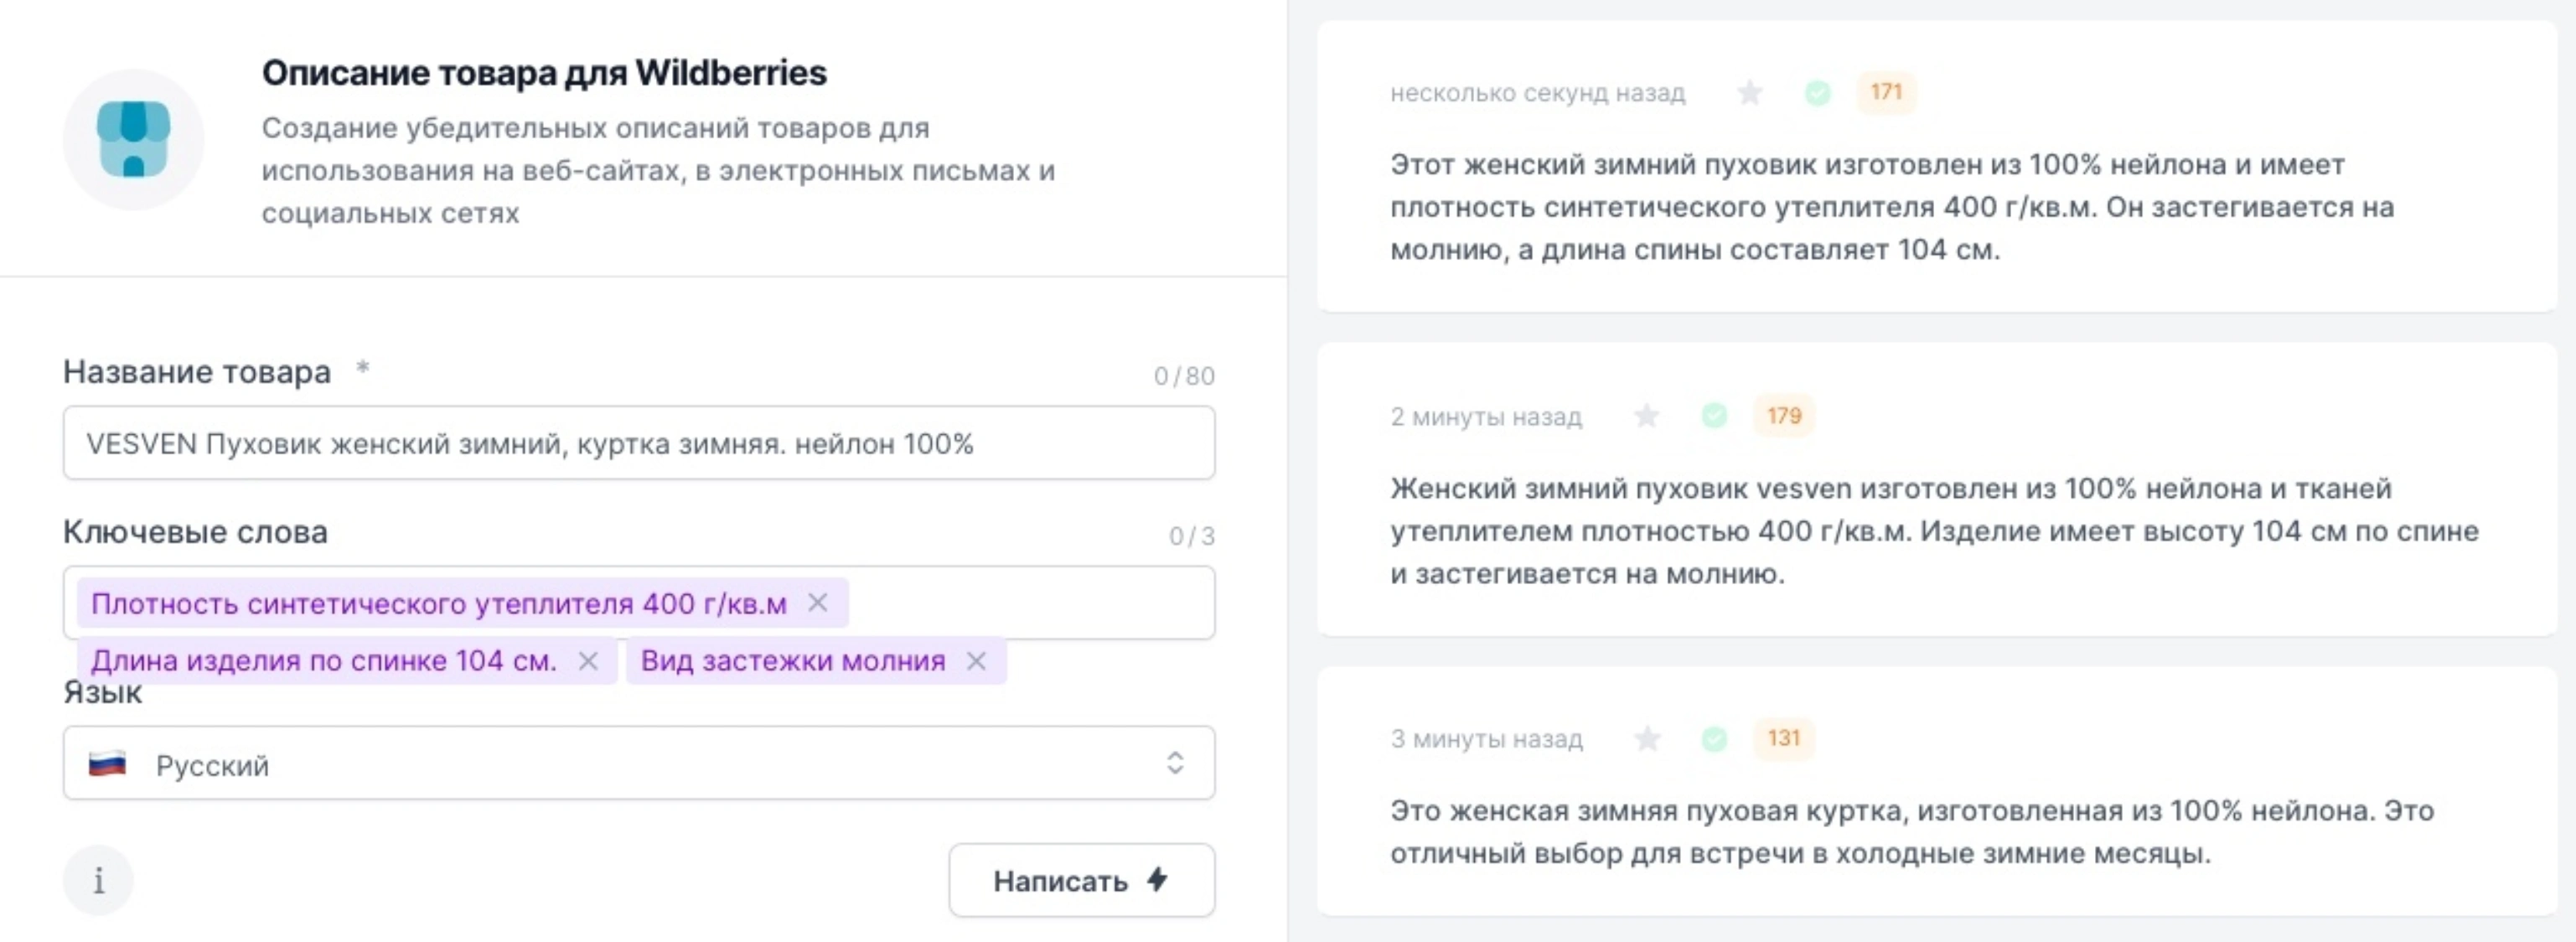
\includegraphics[scale=0.15]{gerwin.png}
	\caption{Сервис Gerwin.}
	\label{fig:gerwin}
\end{figure}

\newpage
\subsection{CopyMonkey}

CopyMonkey — создает описания для товара по его характеристикам и ключевым словам \cite{copymonkey}.

Преимущества данного сервисы:
\begin{itemize}
	\item высокая скорость генерации (1-2 секунды);
	\item доступны бесплатные ежедневные попытки;
	\item разные описания к одному товару на выбор.
\end{itemize}

Недостатки:
\begin{itemize}
	\item низкое качество текста, нейросеть просто сгруппировала характеристики;
	\item есть логические несостыковки в тексте;
	\item один вариант описания товара без возможности выбора.
\end{itemize}

На рисунке \ref{fig:copymonkey} представлен интерфейс данного сервиса.

\begin{figure}[ht]
	\centering
	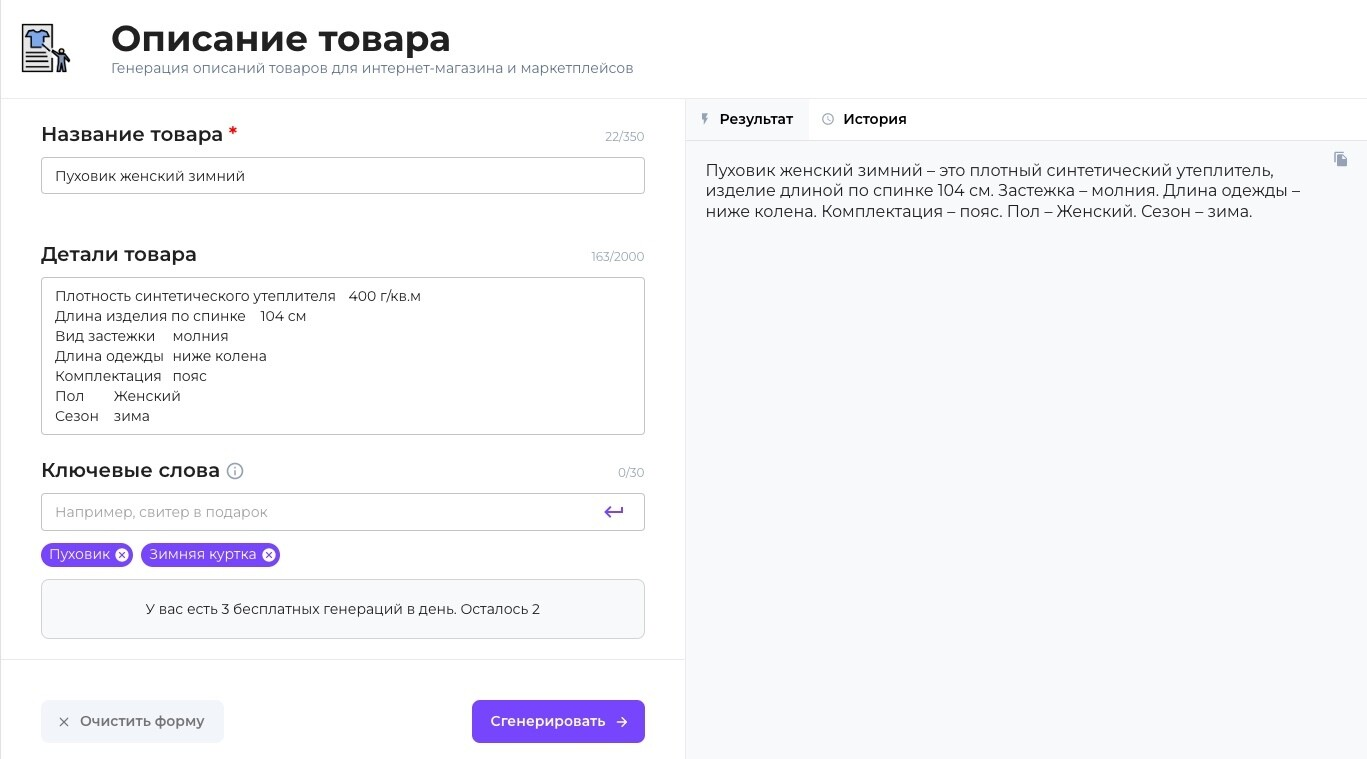
\includegraphics[scale=0.35]{copymonkey.png}
	\caption{Сервис CopyMonkey.}
	\label{fig:copymonkey}
\end{figure}

\newpage
\subsection{Сравнительный анализ существующих решений}

TurboText.Pro генерирует более развернутое описание товара, но есть пара неточностей, которые легко поправить, потратив на это не больше минуты. После описание можно размещать в карточке товара интернет-магазина или на маркетплейсе. CopyMonkey и Gerwin справляются со своей задачей хуже. Все три сервиса можно протестировать бесплатно и выбрать тот, который подходит для работы лучше всего.

Сравнительный анализ существующих решений может быть представлен в таблице \ref{compare_exist}.

\begin{table}[h]
	\centering
	\begin{tabular}{ | l | l | l | l | }
		\hline
		Сервис & Стоимость & Генерация & Качество \\
		& & по фотографии & генерации \\ \hline
		TurboText.Pro & Бесплатно & + & Высокое  \\ \hline
		Gerwin & Бесплатно & — & Среднее \\ \hline
		Copymonkey & Бесплатно & — & Низкое \\
		& 3 попытки в день &  &  \\ \hline
	\end{tabular}
	\caption{Cравнение существующих решений по генерации SEO-описания товара.}
	\label{compare_exist}
\end{table}


\newpage
\section{Данные} 

Для достижения поставленной цели и задач проекта, данные должны удовлетворять следующим требованиям:
\begin{itemize}
	\item данные должны быть достоверными и правильно отражать характеристики товаров;
	\item данные должны иметь четкую классификацию товаров по категориям и подкатегориям, соответствующих структуре категорий маркетплейсов в РФ (например, «Ozon» или «Wildberries»);
	\item данные должны быть структурированы в удобном для обработки формате, таком как CSV, JSON или в виде базы данных;
	\item данные должны включать фотографии товаров с разных ракурсов и в различных вариациях, а также иметь их текстовые описания;
	\item необходимо иметь достаточное количество данных для каждой категории товаров, чтобы обеспечить репрезентативность для анализа и обучения моделей;
	\item данные должны быть актуальными и регулярно обновляемыми для отражения текущих трендов и состояния рынка.
\end{itemize}

На данный момент существуют несколько датасетов для работы с товарами, взятых с интернет-магазинов электронной торговли:
\begin{itemize}
	\item Fashion-MNIST — набор данных, используемый для категоризации товаров. Он содержит почти 60 000 обучающих изображений и 10 000 тестовых изображений одежды и аксессуаров, разделенных на 10 категорий: футболка, брюки, свитер, платье, пальто, сандалии, рубашка, кроссовки, сумка и ботинки. Каждое изображение имеет размер 28x28 пикселей и представлено в оттенках серого \cite{fashion_mnist}.
	\item Innerwear Data from Victoria's Secret and Others — набор данных, включающий информацию более чем о 600 000 товарах нижнего белья, собранных из популярных торговых точек. В этот набор входят описания продуктов, цены, категории и рейтинги \cite{victoria_secret_data}.
	\item eCommerce Item Data — набор данных, включающий артикулы и соответствующие описания продуктов из каталога бренда верхней одежды. Эти данные отлично подходят для использования в рекомендательных системах \cite{eсommerce_item_data}.
	\item Fashion Products on Amazon — набор данных, созданный на основе извлеченной информации с Amazon. Он включает около 22 000 товаров и содержит описания продуктов, цены, категории и рейтинги \cite{amazon_data}.
\end{itemize}

Поскольку в открытых источниках не имеется удовлетворяющего всем требованиям датасета, данные для поставленной задачи собирались самостоятельно. Был проведен анализ на возможность парсинга наиболее популярных маркетплейсов в РФ «Ozon» и «Wildberries».

\begin{table}[h]
	\centering
	\begin{tabular}{ |l|l| }
		\toprule
		\multicolumn{1}{c}{\textbf{Анализ парсинга «Ozon»}} & \multicolumn{1}{c}{\textbf{Анализ парсинга «Wildberries»} } \\
		\midrule		 
		Сильная защита, частая блокировка  &  Слабая защита, не требуется смена  \\
		пользователей, смена userAgent не всегда  & userAgent. \\
		помогает. & \\ \hline
		Динамический контент страниц и ленивая & Динамический контент страниц и ленивая\\ 
		подгрузка, что создает трудности при & подгрузка, что создает трудности при\\ 	
		парсинге, вынуждая «прокручивать» экран & парсинге, вынуждая «прокручивать» экран \\
		вниз. & вниз.\\
		 &  \\
		 & Динамическая подгрузка отзывов, которая\\
		 & усложняет скачивание фотографий из них.\\ \hline		
		Огромное количество категорий и & Приемлемое количество категорий и\\
		подкатегорий. & подкатегорий. \\ \hline
		Большая вариативность описания, нет & Единое оформление карточки товара,\\
		единого шаблона для парсинга. Так & упрощает парсинг товара: его описание,\\
		например, когда-то вместо текстов могут & характеристики, фотографии из seo и\\
		быть просто картинки или описание товара & из отзывов. \\
		сопряженно с картинкой. & \\ \hline 
	\end{tabular}
	\caption{Сравнительный анализ маркетплейсов «Ozon» и «Wildberries»}
	\label{table:marketplace_analysis}
\end{table}

Таким образом, было принято решение писать ВКР для продавцов, использующих «Wildberries», так как он является наиболее популярным среди продавцов, а также легче подается парсингу. Данные собирались согласно особенностям структуры этого маркетплейса. Для удобства введем некоторые термины, которыми будем оперировать далее:
\begin{itemize}
	\item \textbf{Карточка товара} – это страница продукта на маркетплейсе, где размещена информация о товаре, фотографии, описание цены и кнопка «Купить».
	\item \textbf{Конечная категория} – это категория, на которых располагаются карточки товаров.
	\item \textbf{Материнская категория} – это категория, которая содержит конечные и материнские категории и на которой не располагаются карточки товаров.
\end{itemize}

Каталог «Wildberries» разделен на категории, в которых размещены карточки товаров одного типа. Категории выстроены по принципу дерева. Есть основные «широкие» категории, такие как «Женщинам», «Дом», «Продукты», которые объединяют внутри себя более мелкие подкатегории. Например, в разделе «Дом» имеются подкатегории «Ванная», «Кухня», «Спальня» и тд, которые в свою очередь могут подразделяться на еще более маленькие подкатегории. 

Требуемые данные располагались на товарных карточках, в которые можно попасть только зная конечную категорию товара. Поэтому было принято решение разделить сбор данных на 2 этапа. На первом этапе был произведен сбор всех имеющихся на «Wildberries» конечных категорий. На втором – сбор необходимой информации с карточек товаров.

\subsection{Этап 1}\label{subsection:datastep1}

«Wildberries» предлагает 22 основные категории (см. рисунок~\ref{fig:wildberries1}), из которых одна является конечной категорией. Данные категории в дальнейшем будем называть категориями первой вложенности. Их подкатегории, соответственно, будут называться категориями второй вложенности. И так далее, спускаясь все ниже по дереву категорий. Экспериментальным путем была выявлена максимальная глубина вложенности – 5.

\begin{figure}[hbtp]
	\centering
	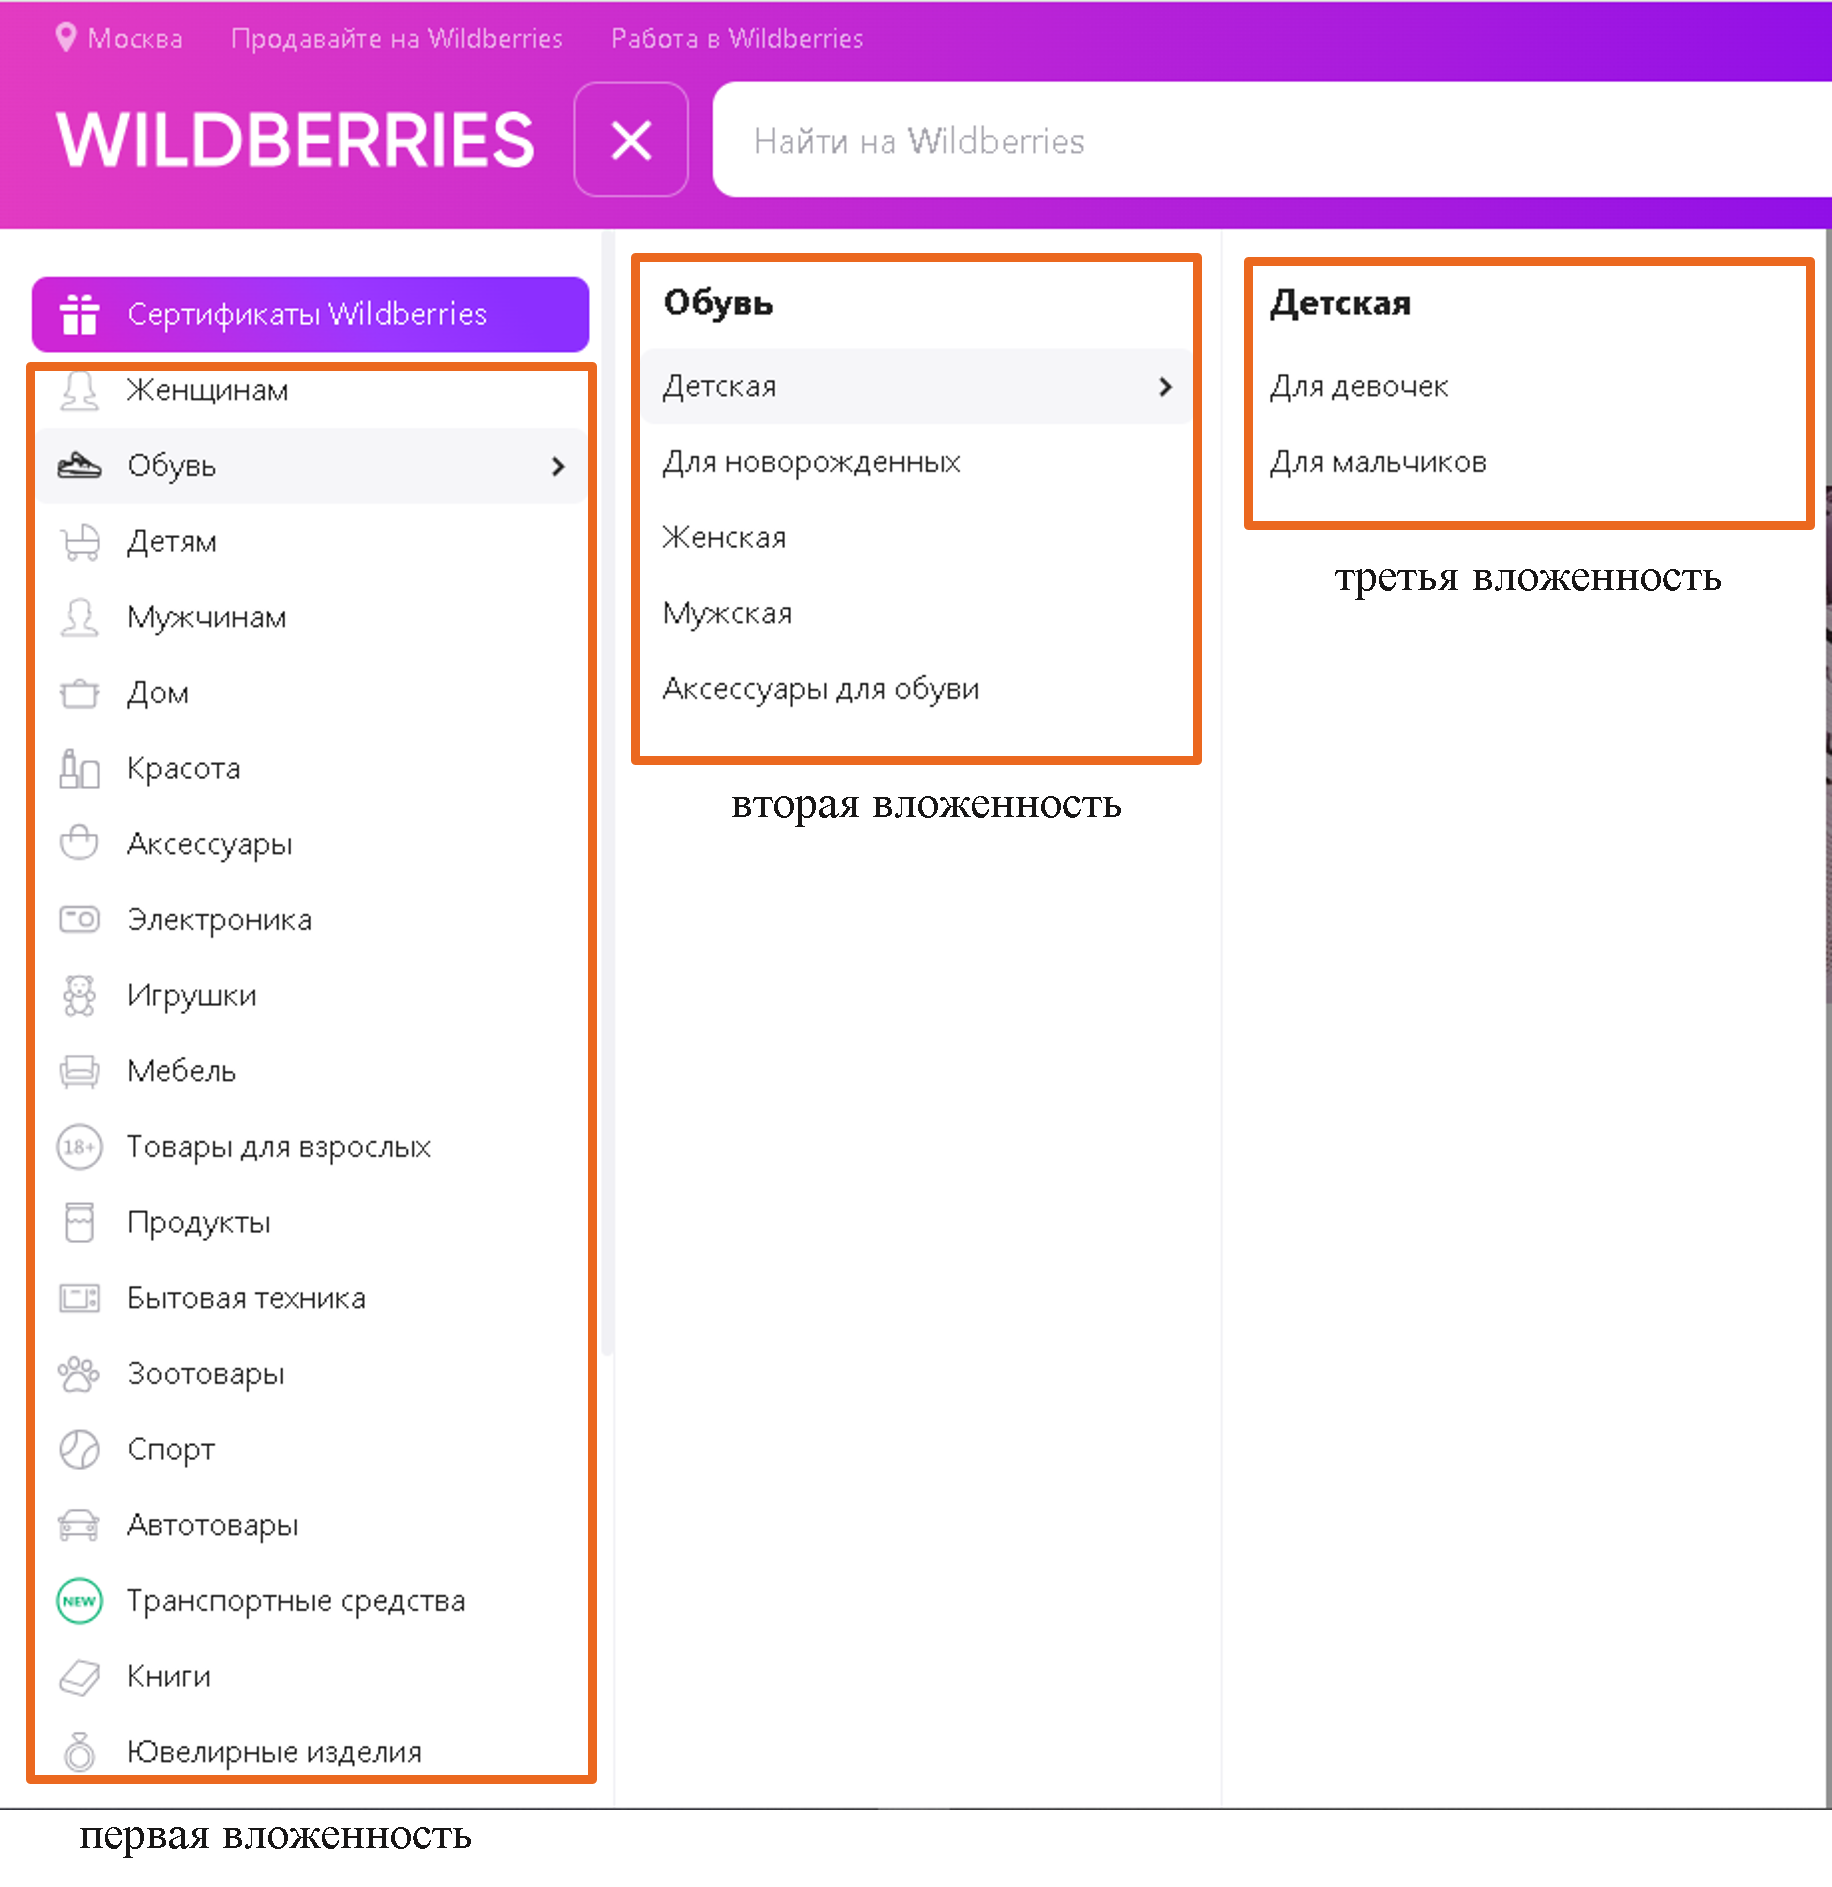
\includegraphics[scale=0.8]{wildberries1.png}
	\caption{Структура каталога «Wildberries» на примере категории «Обувь».}
	\label{fig:wildberries1}
\end{figure} 

Для правильного формирования таргета для классификации при сохранении ссылки на конечную категория нужно было учитывать весь путь по дереву категорий, начиная с первой вложенности. Решением данной задачи стало создание таблицы, где отражалось какие категории было предшествовавшими конкретной конечной категории (см. таблицу~\ref{table:datastatistic0}). При отсутствии более глубокой вложенности на месте данных категорий ставились «NaN». Таким образом, было собрано 1668 конечных категорий.

\begin{table}[ht]
\caption{Фрагмент таблицы, полученной после первого этапа сбора данных.}
\label{table:datastatistic0}
\footnotesize
\centering
	\begin{tabular}{lrrrrr}
		\toprule
		{} & \multicolumn{1}{c}{$\mathsf{category_1}$} &\multicolumn{1}{c}{$\mathsf{category_2}$} &  \multicolumn{1}{c}{$\mathsf{category_3}$} & \multicolumn{1}{c}{$\mathsf{category_4}$} &  \multicolumn{1}{c}{$\mathsf{category_5}$}\\
		\midrule
		... & ... & ... & ... & ... & ... \\
		437 & Дом & Предметы интерьера & Фоторамки и фотоальбомы & Фотоальбомы       & NaN\\
		438 & Дом & Предметы интерьера & Картины и постеры       & Рамы для постеров & NaN\\
		439 & Дом & Предметы интерьера & Картины и постеры       & Постеры           & Детская тематика\\
		440 & Дом & Предметы интерьера & Картины и постеры       & Картины           & Арт и абстракция\\
		441 & Дом & Предметы интерьера & Картины и постеры       & Постеры           & Фэнтези\\
		... & ... & ... & ... & ... & ... \\
		\bottomrule
	\end{tabular}
	\begin{tabular}{ll}
		\toprule
		{} & \multicolumn{1}{c}{$\mathsf{url}$}\\
		\midrule
		... & ... \\
		437 & https://www.wildberries.ru/catalog/dlya-doma/predmety-interera/fotoramki-i-fotoalbomy/fotoalbomy\\
		438 & https://www.wildberries.ru/catalog/dlya-doma/predmety-interera/kartiny/ramy-dlya-posterov\\
		439 & https://www.wildberries.ru/catalog/dlya-doma/predmety-interera/kartiny/postery/detskaya-tematika\\
		440 & https://www.wildberries.ru/catalog/dlya-doma/predmety-interera/kartiny/kartiny/art-i-abstraktsiya\\
		441 & https://www.wildberries.ru/catalog/dlya-doma/predmety-interera/kartiny/postery/fentezi\\
		... & ... \\
		\bottomrule
	\end{tabular}
\end{table}


Составление данной таблицы производилось посредством парсинга данных с сайта «Wildberries» через Python с использованием библиотек selenium и BeautifulSoup. Блокировок со стороны маркетплейса замечено не было. Особенность и неудобством парсинга была динамическая подгрузка страниц, которая вынуждала выдерживать паузы в несколько секунд для удовлетворяющей прогрузке страницы. Данное обстоятельство привело с значительному увеличению времени парсинга данных.

При анализе собранной таблицы были выявлены некоторые особенности категориальной политики «Wildberries». Во-первых, категории у данного маркетплейса не фиксированы. Например, было отмечено, что часть категорий активно перемещается из раздела в раздел, какие-то категории могут пропадать, также могут появляться новые категории. Данные, собранные в текущем датасете, актуальны на конец января 2024 года. Однако для поддержания списка категорий в актуальном состоянии необходимы механизмы регулярного обновления данных. Во-вторых, на маркетплейсе имеются конечные категории, ссылающиеся на одни и те же url страницы. Подобные категории будут называться дублирующими. Подобные дубляжи могли иметь разное происхождение: особенности маркетинга и неудачное время парсинга, выпавшее на перемещение категорий. С точки зрения маркетинга подобные дублирования оправданы, поскольку потенциальный покупатели могут по своим соображениям относить одни и те же товары к разным категориям. Для примера, категория «Коврики» находилась в разделе «Автотовары\_Коврики» и «Электроника\_Автоэлектроника\&и\&навигация\_Коврики». Для корректной работы модели была написана отдельная процедура удаления подобных дублирующих категорий. Выбор, какой из дубликатов оставлять, производился вручную. Всего было найдено 69 дублирующих ссылок, которые могли встречаться 2 и более раза. Таким образом, после удаления в таблице осталось 1580 категорий.

Далее можно было переходить ко 2му этапу.


\subsection{Этап 2}\label{subsection:datastep2}

Второй этап сбора данных заключался в прохождении по собранному ранее списку конечных категорий и сбора из каждой из них информации с карточек товаров. Было принято решение брать по 20 товаров из каждой конечной категории. Из каждой карточки товара сохранялось первое фотография от продавца, первая фотография из отзыва и описание товара (см. рисунок~\ref{fig:wildberries2}). Первая фотография от продавца бралась по причине ее обязательного присутствия в карточке товара, а также гарантированного качественного изображения товара на ней. Однако поскольку разрабатываемый сервис рассчитан на работу в большинстве случаев с фотографиями от пользователей, все дефекты, присущие любительским фотографиям могут иметь место быть. Поэтому для стабильности предсказаний классификационной модели, было решено подавать в нее также фотографии из отзывов, которые максимально близко будут похожи на фотографии, с которыми будет работать в дальнейшем сервис. Описания товара были нужны для задачи генерации текстовых описаний к изображениям. В итоге при полном наборе для каждой конечной категории имелось 40 фотографий (20 фотографий от продавцов и 20 фотографий из отзывов) и 20 описаний.

\begin{figure}[hbtp]
	\centering
	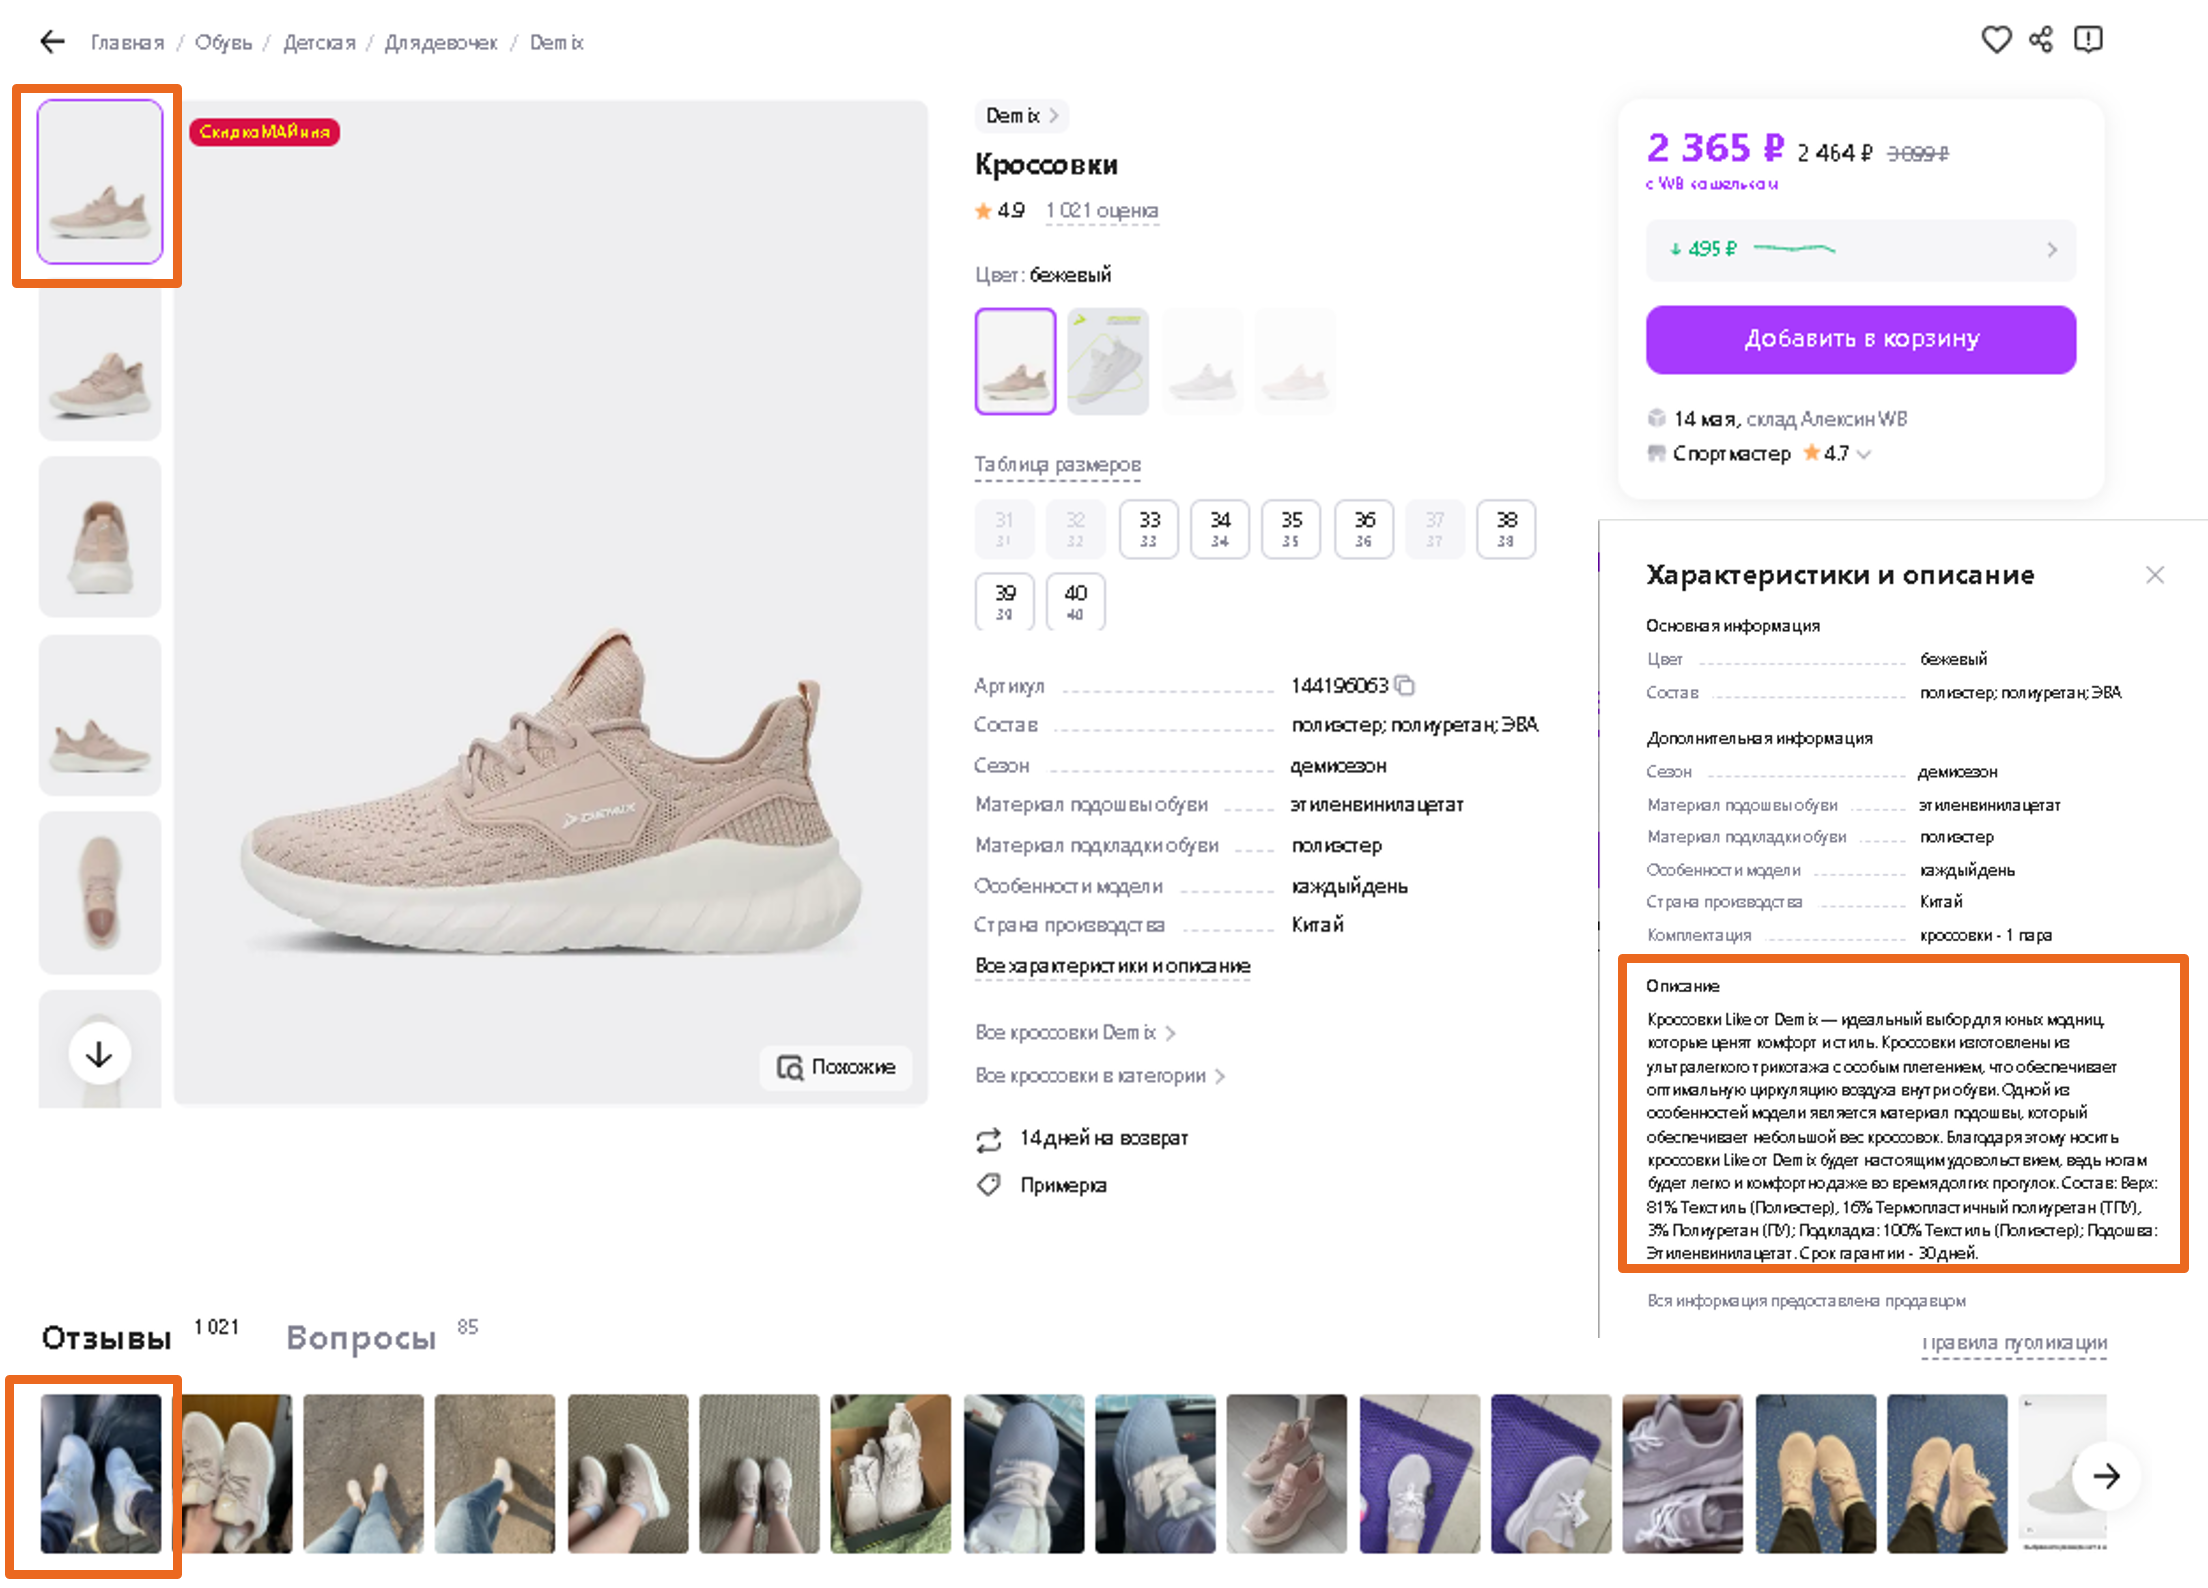
\includegraphics[scale=0.8]{wildberries2.png}
	\caption{Пример карточки товара на «Wildberries». Верхний левый прямоугольник – первая фотография от продавца. Нижний левый прямоугольник – первая фотография из отзыва. Правый прямоугольник – текстовое описания товара.}
	\label{fig:wildberries2}
\end{figure}

При выполнении данного этапа было несколько трудностей. Во-первых, стандартная на «Wildberries» динамическая прогрузка страниц, увеличивающая время парсинга более чем в 3 раза. Приходилось делать паузы при открытии страницы с карточкой товара, при открытии описания, лежащее в отдельной вкладке, и пролистывание страницы вниз для подгрузки информации об отзывах. Примерное время парсинга данных, затраченное на второй этап, равнялось 2м неделям. Во-вторых, имели товары с меткой «18+», для которых требовалось дополнительное нажатие кнопки, подтверждающее достижение указанного возраста. В-третьих, некоторые поля в карточке товара заключали в себе картинки, которые вынуждали в определенных случаях дополнительно пролистывать страницу вниз. В-четвертых, для нажатия кнопки с целью получения описание к товару, выдвигалось требование расположение кнопки в зоне видимости экрана. Это приводило к еще более тонкой настройке пролистывания страницы, подобранной под конкретный размер экрана компьютера.

Для сохранения данных из карточек товара была придумала специальная структура с целью дальнейшего удобства использовании в задаче классификации и генерации текста. Все товары, собранные из одной конечной категории, сохранялись в отдельную папку, содержащую следующие элементы:
\begin{itemize}
	\item папку «card», куда складывались фотографии от продавцов
	\item папку «feedbacks», куда складывались фотографии из отзывов
	\item файл «descriptions.csv», где сохранялись описания к товарам
\end{itemize}

Название данной папки определялось посредство таблицы 1 и складывалось из всех материнских категорий, участвовавших в пути к конечной категории. Например, для конечной категории «Фотоальбомы» (см. таблицу~\ref{table:datastatistic0}) название папки было следующее: \\ «Дом\_Предметы\&интерьера\_Фоторамки\&и\&фотоальбомы\_Фотоальбомы», а для категории «Фэнтези» - «Дом\_Предметы\&интерьера\_Картины\&и\&постеры\_Постеры\_Фэнтези». Более подробно об использовании подобной структуры ранения данных будет описание в разделе \ref{subsection:results-classification}.

Первичный анализ собранных данных выявил, что не у всех товаров имелись отзывы с фотографиями и описания. Описания имелись в 99.8\% проценте случаев. В таблице~\ref{table:datastatistic1} приведены некоторые статистические данные о собранных фотография от продавца и из отзыва. Можно заметить, что некоторые конечные категории были полностью без фотографий в отзывах. Однако, опираясь на перцентили, можно сделать вывод, что таких категорий было довольно мало. Касательно фотографий от продавцов можно сделать 2 вывода. Во-первых, есть категории, представленные менее чем 20ю товарами. Во-вторых, есть как минимум одна категория, в которой имеется только 1 товар. Подобные категории нас не устраивают, потому что далее будет производиться деление каждой категории на 2 части, и категории с одним товаром невозможно будет разделить.

\begin{table}[ht]
	\caption{Описательная статистика по фотографиям от продавца (столбец «card») и фотографиям из отзыва (столбец «feedbacks»).}
	\label{table:datastatistic1}
	\footnotesize
	\centering
	\begin{tabular}{l|rr}
		\toprule
		{} & \multicolumn{1}{c}{$\mathsf{card}$} & \multicolumn{1}{c}{$\mathsf{feedbacks}$}\\
		\midrule
		count &	1580  & 1580\\
		mean  & 19.98 & 17.72\\
		std   & 0.63  &	4.23\\
		min   &	1     &	0\\
		25\%  &	20    &	18\\
		50\%  &	20    &	19\\
		75\%  &	20    &	20\\
		max   &	20    &	20\\
		\bottomrule
	\end{tabular}
\end{table}

Всего категорий, представленных менее 20 товарами, было выявлено 5 штук (см. таблицу~\ref{table:datastatistic2}). Из них представляли наибольший интерес \\ "Мебель\_Офисная\&мебель\_Перегородки\&офисные" и \\ "Дом\_Освещение\_Лифты\&для\&люстр", из-за чересчур малого количества товаров. Категорию с одним товаром было решено удалить. Таким образом, осталось 1579 конечных категорий, с которыми шла вся дальнейшая работа.

\begin{table}[ht]
	\caption{Таблица с категориями, имеющими менее 20 товаров.}
	\label{table:datastatistic2}
	\footnotesize
	\centering
	\begin{tabular}{rc}
		\toprule
		\multicolumn{1}{c}{кол-во товаров} & \multicolumn{1}{c}{категория}\\
		\midrule
		18 & Дом\_Кухня\_Кухонный\&текстиль\_Чехлы\&для\&ручек\&холодильников\\
		4  & Дом\_Освещение\_Лифты\&для\&люстр\\
		19 & Мебель\_Гардеробная\&мебель\_Ящики\\
		1  & Мебель\_Офисная\&мебель\_Перегородки\&офисные\\
		19 & Мебель\_Офисная\&мебель\_Шкафы\\
		\bottomrule
	\end{tabular}
\end{table}

При более детально рассмотрении собранных данных было замечено, что фотографии из отзывов довольно шумные (см. рисунок~\ref{fig:dataexample1}). Очень много одинаковых фотографий, фотографий, где не очень понятно, что изображено. Поэтому для дальнейшей работы использовались только фотографии товара от продавца.

\begin{figure}[hbtp]
	\centering
	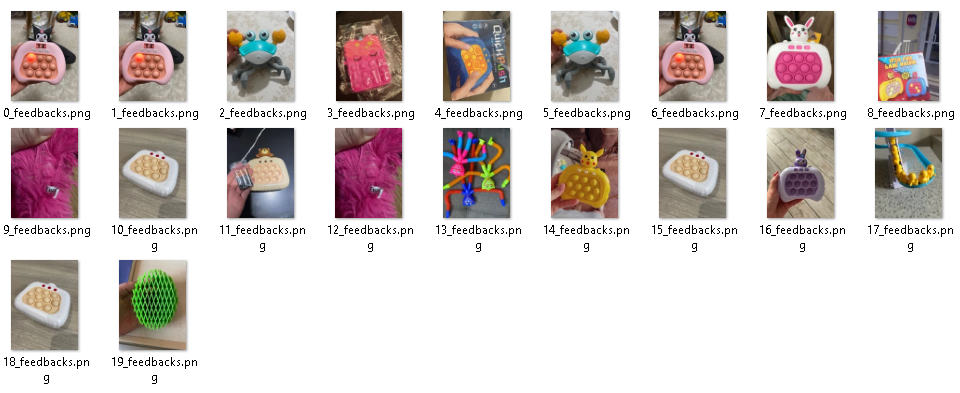
\includegraphics[scale=0.8]{dataexample1.png}
	\caption{Фотографии из отзывов в категории «Игрушки\_Антистресс».}
	\label{fig:dataexample1}
\end{figure}

Далее интересно было рассмотреть количество собранных данных в разрезе категорий первой вложенности (см. рисунок~\ref{fig:amount_of_categoty}). Из круговой диаграммы можно заметить, что категории довольно несбалансированный. Например, категория «Дом» вмещает в себя порядка 6000 пример. В то время как в категории «Ювелирные\&изделия» только 320 примеров.

\begin{figure}[ht]
	\centering
	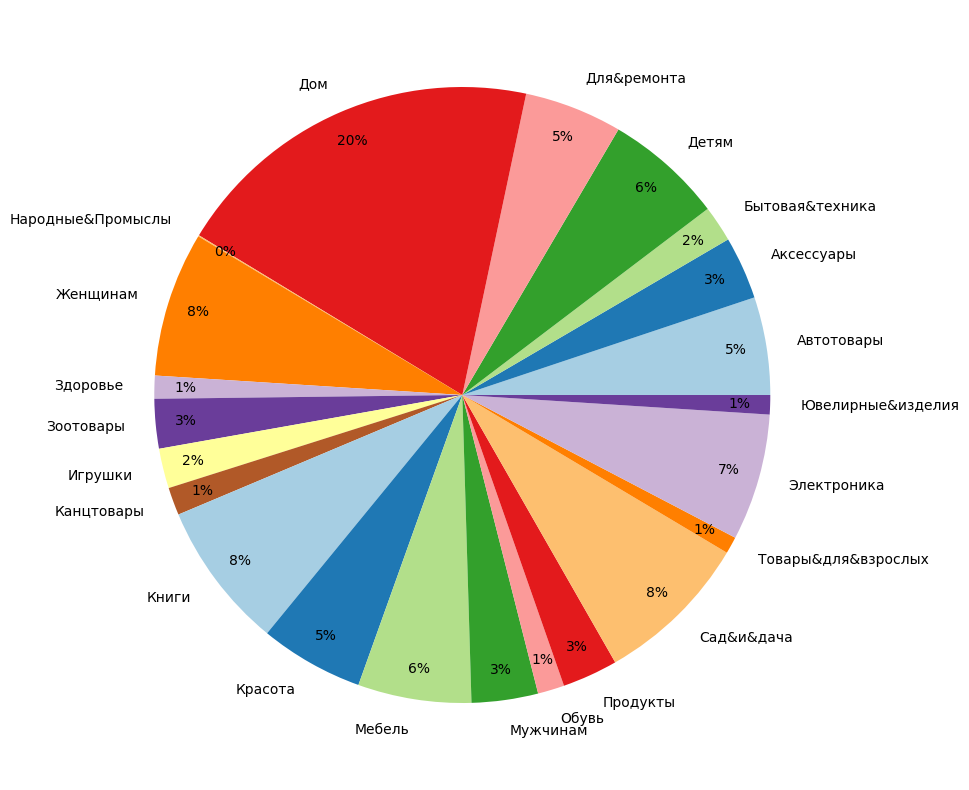
\includegraphics[scale=0.7]{amount_of_categoty.png}
	\caption{Распределение данных по категориям первой вложенности.}
	\label{fig:amount_of_categoty}
\end{figure}

Подобную картину можно наблюдать в категориях всех вложенностей (см. приложение~\ref{appendix:amount_of_categor2}).

После появление базового понимания данных надо было приступать к их детальному изучению. Как правило, парсинг большого количества данных, тем более с постоянно меняющихся маркетплейсов, не проходит идеально. В сохраненных данных могут быть оплошности, которые помешают грамотно решать задачу классификации и генерации текста. Приведем некоторые примеры, выявленных особенностей, требуемых принятие решений с нашей стороны:
\begin{itemize}
	\item Встречаются категории, которые с точки зрения категорийного менеджмента, имеют место быть. Одна для классификационной модели машинного обучения такие категории будут не осиливаемыми. Например, в разделе «Женщинам» есть подкатегории «Женщинам\_Белье» и «Женщинам\_Большие\&размеры\_Белье». Если детально изучить фотографии, которые в этих категориях присутствуют, можно сделать вывод, что особых различий между ними нет. Единственное, что было подмечено, что на очень немногих фотографиях стоит надпись «4XL» или что-то подобное, указывающее, что у данного товара имеются большие размера. Более того, в обеих категориях присутствуют одинаковые товары.
	\item В данных попадались «мусорные» категории. Предположительно, подобное возникало из-за изменения url ссылок на категории со стороны «Wildberries». В подобных категориях находились товары, собранные случайным образом из всевозможных категорий с маркетплейса.
	\item Распределение товаров по категориям не очень четкая задача. В связи с этим встречались одинаковые товары, находящиеся в разных категориях. Например, одна и та же продукт мог находиться в категориях «Зоотовары\_Груминг\&и\&уход», «Зоотовары\_Для\&кошек\_Груминг\&и\&уход» и «Зоотовары\_Для\&собак\_Груминг\&и\&уход».
	\item В части материнских категорий встречались разделы «Подарки» (например, материнские категории «Мужчинам\_Подарки\&мужчинам» и \\ «Женщинам\_Подарки\&женщинам»), куда были собраны товары из совершенно разных категорий, таких как «Аксессуары», «Дом», «Продукты» и тд.
	\item Поскольку при парсинге из каждой категории брались первые 20 товаров, появляется неконтролируемый фактор того, какие товары стоят вначале. Как правило, пользователи смотрят только на первые товары в выдаче. Поэтому на маркетплейсах существуют множество механизмов и правил отбора товаров, которые будут показаны пользователю в начале. В нашем случае было замечено, что некоторые категории стали более шумными из-за сезонных товаров. Например, в категории «Зоотовары\_Фермерство» были найдены пасхальные яйца.
	\item Бывали категории, которые по смыслу имели место быть как отдельные категории, однако в них были собраны не совсем подходящие товары. Например, в категории «Мужчинам\_Религиозная\_Православие» находились обычные рубашки и штаны, часть из которых присутствовала также в категории «Мужчинам\_Рубашки» и\\ «Мужчинам\_Брюки».
\end{itemize}

Приведенные особенности сохраненных данных требовали ручной очистки датасета. Необходимо было применять следующие действия: полное удаление категории, удаление конкретной фотографии из отзыва, удаление товара полностью (фотографию от продавца, из отзыва и описание к нему) и произведение полного переноса товара (фотографию от продавца, из отзыва и описание к нему) из одной категории в другую. Для удобства и быстроты данной процедуры были написаны функции, позволяющие механизмами Python вносить изменения в собранные данные.

По окончании данной процедуры было подмечено, что категории требовали очистки в разной степени. Какие-то категории, как «Зоотовары», требовали практически полного переформирования. Другие категории обходились легкой очисткой, например «Продукты». Некоторые категории совсем не требовала вмешательства. Таким образом, финальный датасет стал состоять из 1385 конечных категорий (см. таблицу~\ref{table:datastatistic2}).

\begin{table}[ht]
	\caption{Описательная статистика по фотографиям от продавца после очистки собранных данных. \textsl{Примечание:} статистика по фотографиям из отзывов не приведена, поскольку, как упоминалось ранее, решено было в дальнейшем работать только с фотографиями от продавца.}
	\label{table:datastatistic3}
	\footnotesize
	\centering
	\begin{tabular}{l|r}
		\toprule
		{} & \multicolumn{1}{c}{$\mathsf{card}$}\\
		\midrule
		count &	1385\\
		mean  & 20.31\\
		std   & 3.95\\
		min   &	4\\
		25\%  &	20\\
		50\%  &	20\\
		75\%  &	20\\
		max   &	116\\
		\bottomrule
	\end{tabular}
\end{table}

\newpage
\section{Теоретические основы} 

\subsection{Задача многоклассовой классификации изображений}

Задача многоклассовой классификации изображений заключается в том, чтобы отнести каждое изображение из набора данных к одной из заранее определенных категорий или классов. Для решения задачи необходимо использовать разнообразный набор изображений, каждый из которых должен быть помечен (аннотирован) соответствующим классом.

Для многоклассовой классификации часто используют сверточные нейронные сети, такие как ResNet, MobileNet или EfficientNet (подробнее см. в разделе \ref{classification_models}). Для оценки качества модели обычно применяются следующие метрики: Accuracy, Precision, Recall и F1-score (подробнее см. в разделе \ref{classification_metrics}).

Для повышения производительности модели можно использовать различные методы, например:
\begin{itemize}
	\item тонкая настройка гиперпараметров — корректировка параметров обучения, таких как скорость обучения, размер батча и т.д.
	\item дополнительная аугментация данных — применение различных преобразований к изображениям, таких как повороты, сдвиги, масштабирование, для увеличения разнообразия обучающих данных.
	\item использование предобученных моделей — начинать обучение с модели, предварительно обученной на большом наборе данных, таком как ImageNet.
\end{itemize}

\subsection{Обзор классификаторов изображения}\label{classification_models}

В этом разделе будет дан обзор существующих классификаторов изображений, их архитектурные особенности, а также преимущества и недостатки.
 
\subsubsection{ResNet}

ResNet (Residual Neural Network) — это семейство моделей нейронных сетей, разработанные для решения проблемы затухания градиента \cite{resnet}. Модели получили широкое признание и стали основой для многих современных архитектур благодаря своей способности эффективно тренировать очень глубокие нейронные сети.

Ключевой инновацией ResNet является использование остаточных блоков (от англ. residual blocks), которые помогают бороться с проблемой затухания градиентов в очень глубоких сетях. Основная идея заключается в том, чтобы добавить прямые связи (от англ. skip connections) через несколько слоев, что позволяет градиентам легче проходить через сеть.

Остаточный блок — это компонент архитектуры ResNet, который содержит «обходную связь идентичности», обходящую один или большее количество слоев. Остаточный блок состоит из двух или трех сверточных слоев с прямой связью, которая пропускает входы блока напрямую к его выходу. Это помогает сохранять информацию от предыдущих слоев и упрощает обучение. На рисунке \ref{fig:res-block} представлен пример остаточного блока.

\begin{figure}[ht]
	\centering
	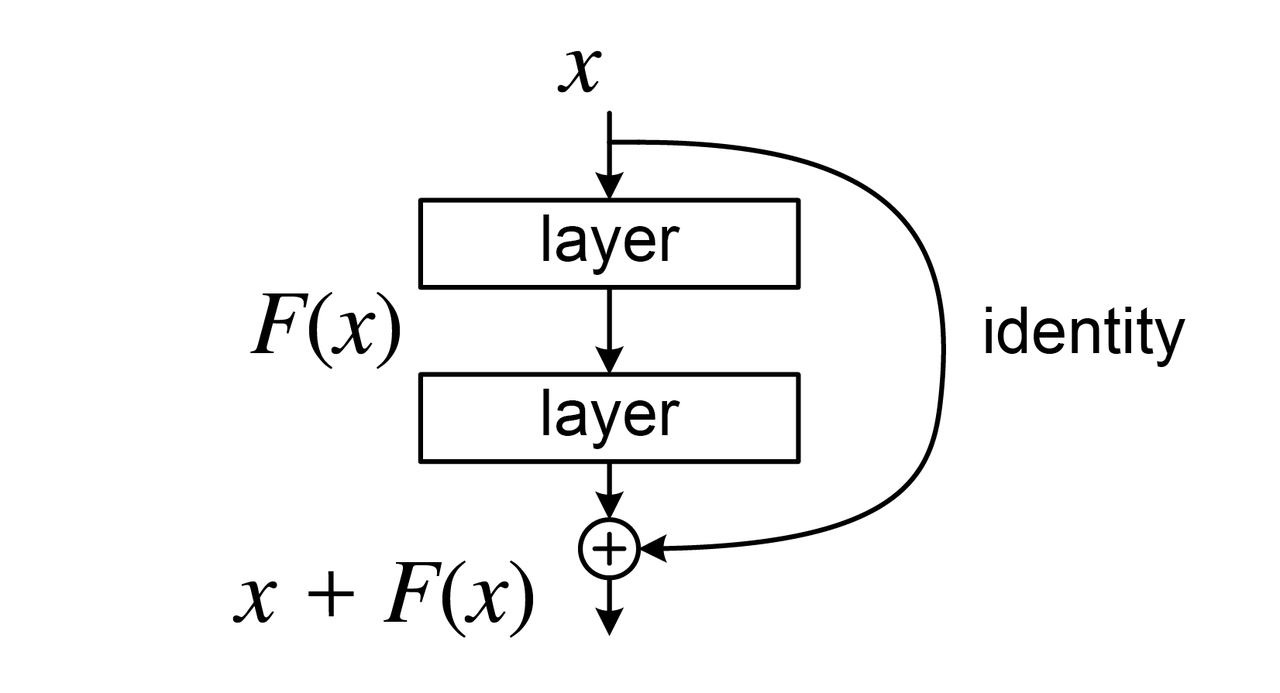
\includegraphics[scale=1.5]{res_block.png}
	\caption{Остаточный блок \cite{resnet}.}
	\label{fig:res-block}
\end{figure}

ResNet предлагает несколько версий моделей с различной глубиной: ResNet-18, ResNet-34, ResNet-50, ResNet-101, ResNet-152. Эти версии различаются количеством остаточных блоков и слоев, что позволяет выбрать модель, соответствующую конкретной задаче и доступным вычислительным ресурсам.

\subsubsection{MobileNet}

MobileNet — это семейство моделей нейронных сетей, специально разработанных для работы на мобильных и встраиваемых устройствах \cite{mobilenet}. Они хорошо оптимизированы и обеспечивают высокую точность при низких вычислительных затратах. MobileNet широко используется в задачах компьютерного зрения, таких как классификация изображений, детекция объектов и сегментация.

Основной инновацией MobileNet является использование глубоких разделяемых сверточных слоев вместо стандартных. Глубокие разделяемые сверточные слои состоят из двух отдельных операций: глубинного свертывания (от англ. depthwise convolution) и точечного свертывания (от англ. pointwise convolution). Глубинное свертывание применяется отдельно к каждому каналу входного изображения, а точечное свертывание используется для объединения выходов глубинного свертывания.

MobileNet использует параметры разложения для управления шириной сети (от англ. width multiplier) и разрешением входного изображения (от англ. resolution multiplier). Width multiplier уменьшает количество каналов в каждой сверточной операции, что снижает количество вычислений и параметров, а resolution multiplier уменьшает размер входного изображения, что дополнительно снижает вычислительные затраты.
 
Благодаря глубинным разделяемым сверточным слоям и параметрам разложения, MobileNet достигает хорошего баланса между производительностью и вычислительными затратами. На рисунке \ref{fig:mobilenet} представлена архитектура MobileNet слоя.


\begin{figure}[ht]
	\centering
	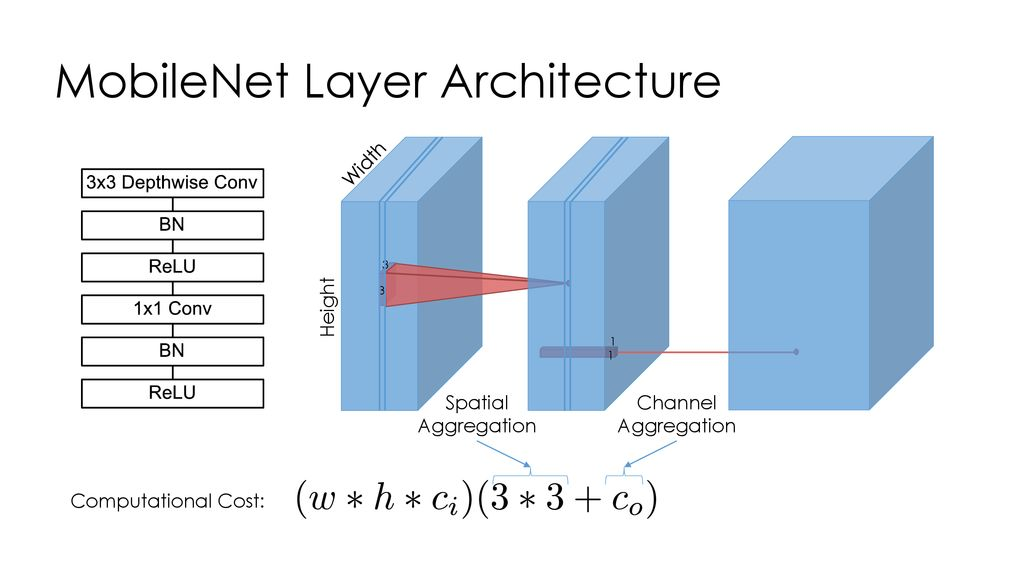
\includegraphics[scale=0.8]{mobilenet.png}
	\caption{Архитектура MobileNet слоя \cite{mobilenet}.}
	\label{fig:mobilenet}
\end{figure}

На данный момент существует несколько версий MobileNet, каждая из которых приносит свои улучшения и оптимизации.

MobileNetV2 — включает улучшения, такие как инвертированные остаточные блоки (от англ. inverted residuals) и линейные узкие слои (от англ. linear bottlenecks) \cite{mobilenetv2}. Эти улучшения помогают сохранять более полезные характеристики признаков и обеспечивают лучшую производительность при тех же вычислительных затратах. Разница между остаточным и инвертированным остаточным блоком представлена на рисунке \ref{fig:mobilenetv2}.

\begin{figure}[ht]
	\centering
	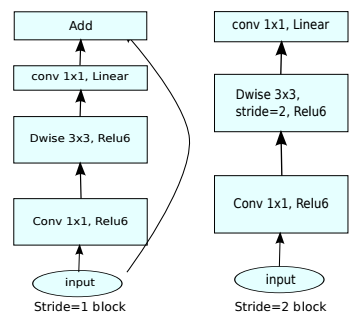
\includegraphics[scale=0.4]{mobilenetv2.png}
	\caption{Разница между остаточным и инвертированным остаточным блоком \cite{mobilenetv2}.}
	\label{fig:mobilenetv2}
\end{figure}

MobileNetV3 — включает дополнительные улучшения, такие как блоки сжатия и возбуждения (от англ. squeeze-and-excitation, SE) и расширенные функции активации \cite{mobilenetv3},  см. рисунок  \ref{fig:mobilenetv3}. Блоки SE позволяют сети лучше фиксировать канальные зависимости в данных, помогает повысить способность модели извлекать значимые функции из входных данных, что приводит к повышению производительности задач распознавания изображений. MobileNetV3 использует расширенные функции активации, такие как h-swish и h-sigmoid. Эти функции обеспечивают более плавные градиенты во время обучения, что может привести к более быстрой сходимости и повышению общей производительности. MobileNetV3 предоставляет две версии: MobileNetV3-Large и MobileNetV3-Small, предназначенные для различных требований производительности и эффективности.

\begin{figure}[ht]
	\centering
	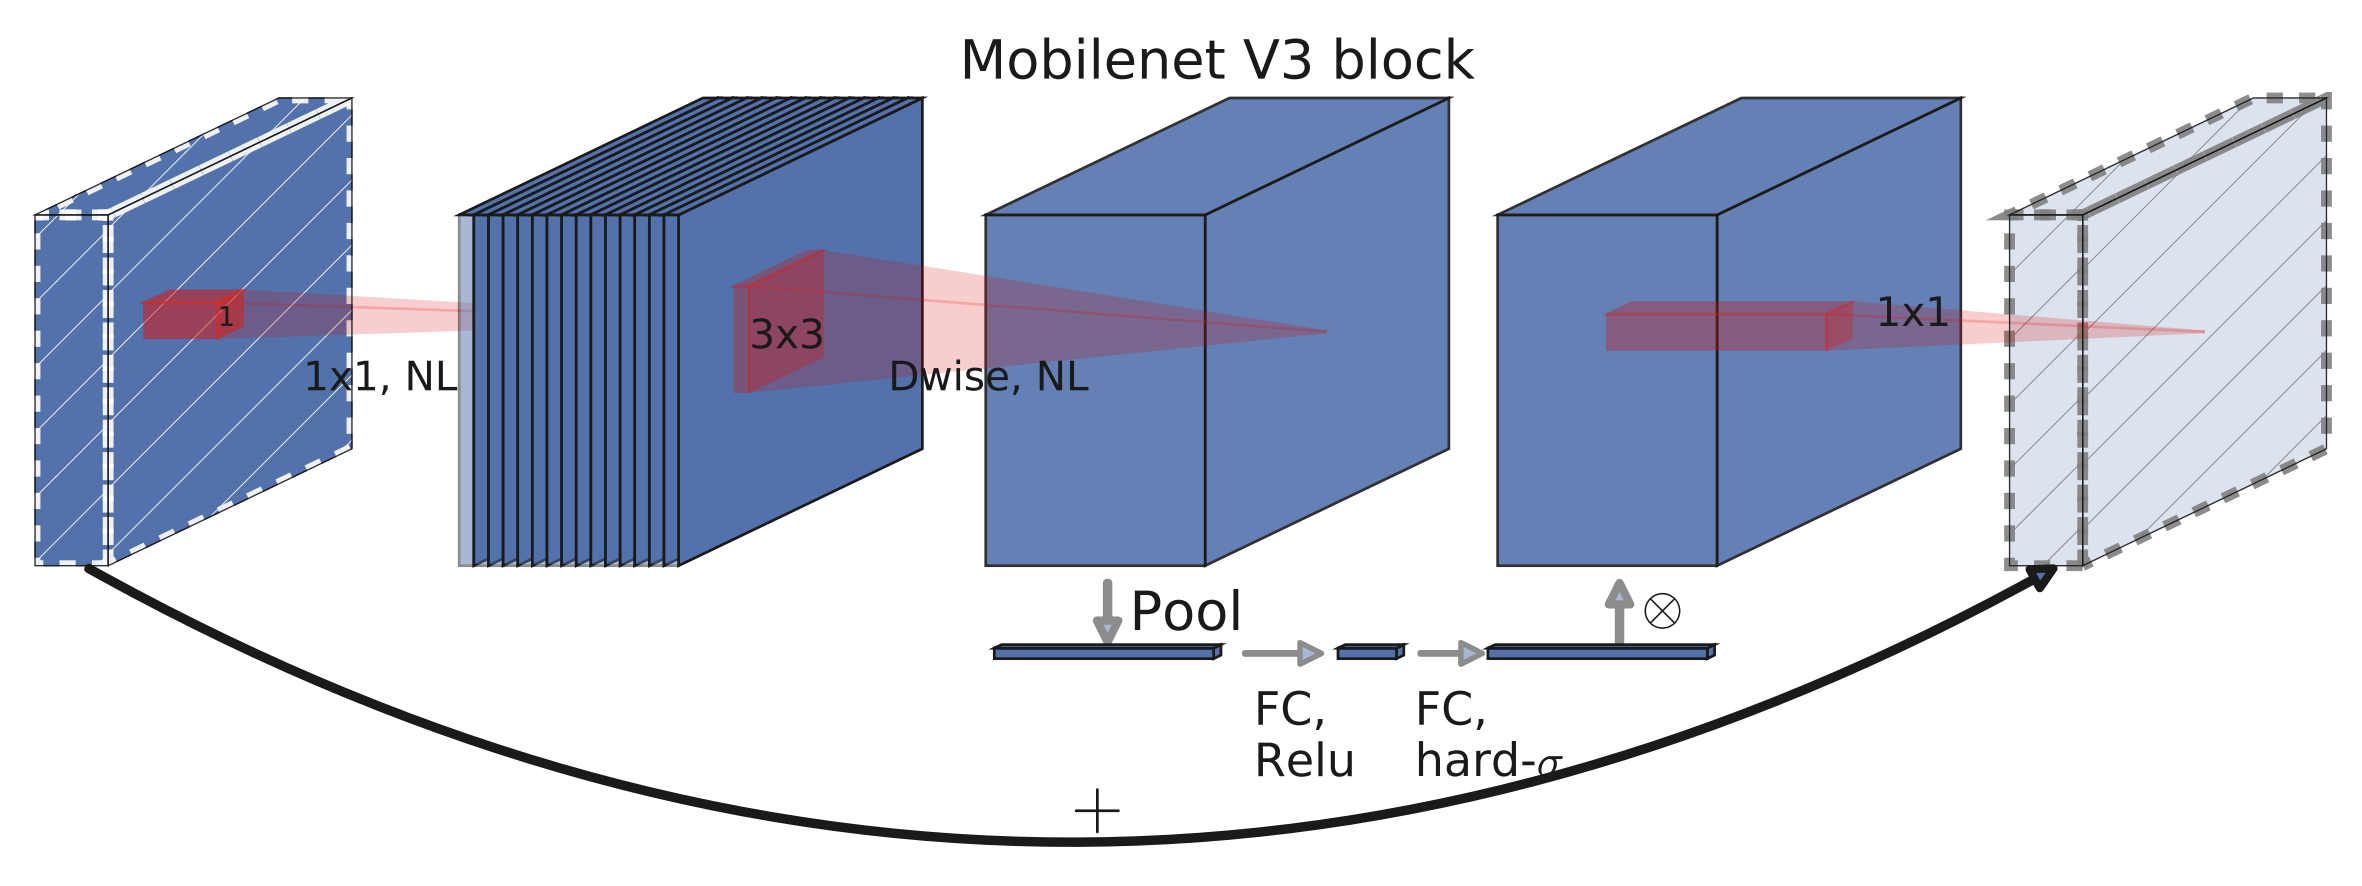
\includegraphics[scale=0.2]{mobilenet-v3-block.png}
	\caption{MobileNetV3 блок \cite{mobilenetv3}.}
	\label{fig:mobilenetv3}
\end{figure}

Однако, несмотря на свою эффективность и компактность, MobileNet в сравнении с более крупными и сложными моделями, такими как EfficientNet, может не достигать такой же высокой точности на некоторых задачах компьютерного зрения.

\subsubsection{EfficientNet}

EfficientNet — архитектура нейронной сети, основанная на идее масштабирования моделей и сбалансированного изменения глубины, ширины (количества каналов) сети, а также разрешения изображений\cite{efficientnet}. Применяется новый метод составного масштабирования (от англ. compound scaling method), который одновременно изменяет глубину, ширину и разрешение с фиксированными пропорциями между этими параметрами. Метод составного масштабирования показан на рисунке \ref{fig:scaling_method}.

\begin{figure}[ht]
	\centering
	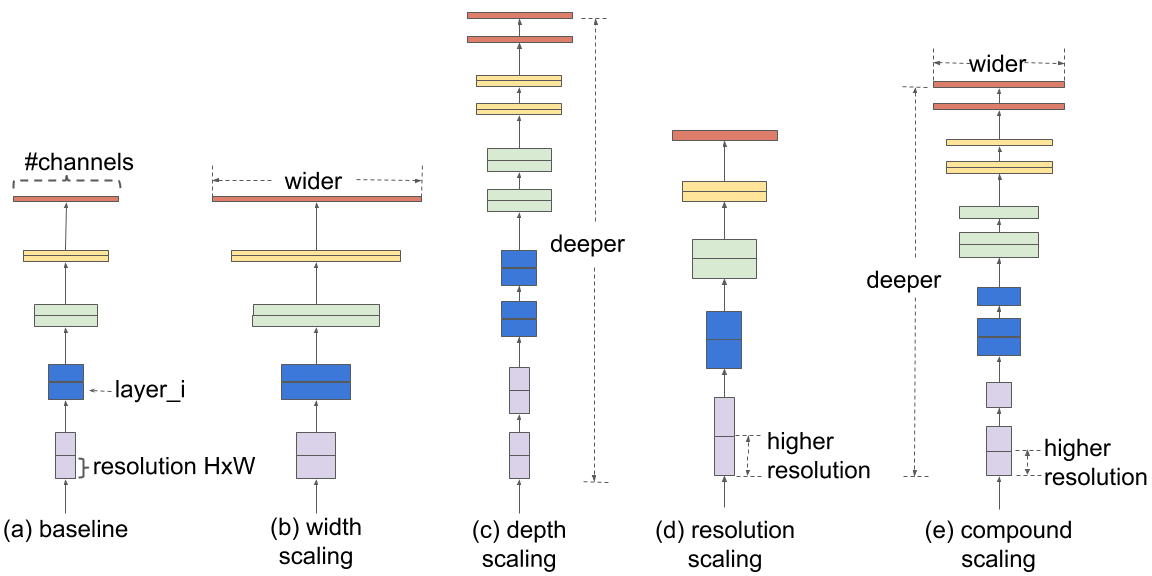
\includegraphics[scale=0.3]{scaling_method.png}
	\caption{Различные методы масштабирования по сравнению со составным\cite{efficientnet}.}
	\label{fig:scaling_method}
\end{figure}

Архитектура EfficientNet состоит из следующих ключевых компонентов:
\begin{enumerate}[label=\arabic*.]
	\item MBConv (англ., Mobile Inverted Bottleneck Convolution) — основной строительный блок EfficientNet, унаследованный из архитектуры MobileNetV2. MBConv включает в себя следующие элементы:
	\begin{itemize}
		\item Pointwise Convolution (1x1) — уменьшает размерность каналов, улучшая вычислительную эффективность.
		\item Depthwise Convolution (3x3 или 5x5) — выполняет свертку по каждому каналу независимо, что значительно снижает количество параметров.
		\item Squeeze-and-Excitation Block — улучшает представление важных характеристик путем адаптивного перенастроя каналов.
	\end{itemize}
	\item Использование функции активации Swish, которая демонстрирует лучшие результаты в глубоких сетях благодаря своей непрерывности и плавности.
	\item Compound Scaling — ключевая концепция EfficientNet, включающая одновременное масштабирование трех аспектов модели:
	\begin{itemize}
		\item Глубина — увеличение количества слоев в сети.
		\item Ширина — увеличение количества каналов в каждом слое.
		\item Разрешение — увеличение разрешения входных изображений.
	\end{itemize}
	Подход compound scaling обеспечивает сбалансированное увеличение модели, что позволяет достигать высокой точности и производительности без чрезмерного увеличения вычислительных затрат, что делает EfficientNet особенно привлекательной для внедрения в мобильные устройства.
\end{enumerate}

Существует несколько версий EfficientNet, каждая из которых разработана для различных применений и требований к вычислительным ресурсам. Оригинальные модели используют простой метод compound scaling, который включает масштабирование глубины, ширины и разрешения изображений с помощью фиксированных коэффициентов. В то время как EfficientNetV2 улучшает этот метод, вводя динамическое масштабирование, которое позволяет более гибко адаптировать модель к различным задачам и условиям. Также EfficientNetV2 использует улучшенные блоки, такие как Fused-MBConv, которые объединяют традиционные MBConv и элементы из ResNet, что позволяет увеличить эффективность обучения и улучшить качество представления данных.

Оригинальные модели EfficientNet (B0 - B7):
\begin{itemize}
\item EfficientNet-B0 — базовая модель, на основе которой построены все остальные версии, использует минимальное количество параметров и вычислительных ресурсов. Архитектура сети представлена на рисунке \ref{fig:efficientnet-b0}
\item EfficientNet-B1 - B7 — модели, которые последовательно масштабируются с использованием compound scaling, увеличивая глубину, ширину и разрешение. Каждая последующая версия обладает большей вычислительной мощностью и точностью по сравнению с предыдущей.
\end{itemize}

\begin{figure}[ht]
	\centering
	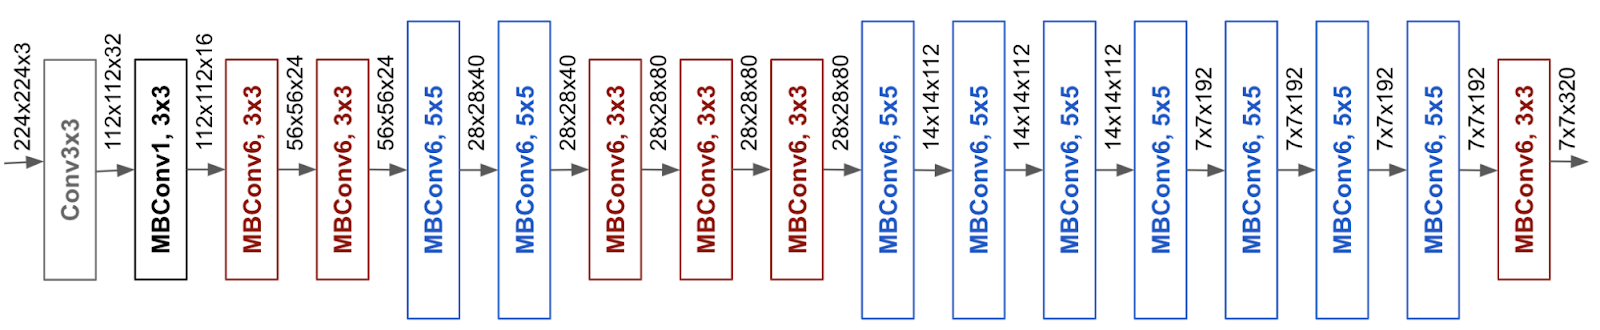
\includegraphics[scale=0.3]{efficientnet-b0.png}
	\caption{Архитектура базовой сети EfficientNet-B0\cite{efficient-b0}.}
	\label{fig:efficientnet-b0}
\end{figure}

Модели EfficientNetV2 (S, M, L):
\begin{itemize}
\item EfficientNetV2-S — оптимизированная версия для мобильных устройств, характеризующаяся компактностью и высокой эффективностью. Подходит для приложений, где критичны вычислительные ресурсы и время отклика.
\item EfficientNetV2-M — средняя версия, предлагающая баланс между производительностью и вычислительными затратами. Часто используется в серверных и облачных средах.
\item EfficientNetV2-L — наиболее мощная версия, предназначенная для задач, требующих максимальной точности и производительности. Используется в высокопроизводительных системах и приложениях с большими объемами данных.
\end{itemize}

Благодаря продуманному подходу к масштабированию, все версии EfficientNet демонстрируют высокую точность на стандартных наборах данных, таких как ImageNet. Стоит отметить, что модели EfficientNetV2 значительно превосходят оригинальные модели EfficientNet. Так например, EfficientNetV2-M снижает параметры на 17 \%, а количество операций ввода-вывода — на 37 
\%, но при этом работает в 4.1 раза быстрее при обучении и в 3.1 раза быстрее при выводе, чем EfficientNet-B7. Кроме того, EfficientNetV2 обеспечивает лучшую точность при значительно меньшем времени выполнения, чем предыдущие модели ConvNet и Vision Transformers на ImageNet \cite{efficientnetv2}. Несмотря на высокую производительность, EfficientNetV2 не использует механизм внимания, как ViTs, что может быть недостатком в некоторых случаях. 

\subsubsection{Vision Transformers}

Визуальные трансформеры (от англ. Vision Transformers, ViTs) – класс моделей глубокого обучения, которые представляют собой архитектуру в области компьютерного зрения, адаптированную из трансформеров, широко используемых в обработке естественного языка \cite{vit}. Основная идея заключается в разделении изображения на небольшие патчи (части), которые затем обрабатываются как токены последовательности в модели трансформера. ViTs используют механизм самовнимания для анализа изображений, что позволяет моделям эффективно захватывать глобальные и локальные зависимости в данных. Vision Transformers достигли выдающихся результатов в задачах классификации изображений.

Архитектура Vision Transformers состоит из следующих этапов (см. рисунок \ref{fig:vit}):
\begin{enumerate}[label=\arabic*.]
	\item Разделение на патчи. Изображение делится на небольшие патчи фиксированного размера (например, 16x16 пикселей), которые затем выравниваются в одномерные векторы. Каждый патч рассматривается как токен в последовательности.
	\item Линейное преобразование патчей. Каждому патчу сопоставляется эмбеддинг фиксированной размерности с помощью линейного слоя. Этот шаг аналогичен созданию эмбеддингов для слов в задачах NLP.
	\item Добавление позиционных эмбеддингов. Поскольку трансформеры изначально не содержат информации о позиции токенов, то к эмбеддингам патчей добавляются позиционные эмбеддинги, которые кодируют пространственное положение каждого патча в исходном изображении.
	\item Последовательность патчей передается через многослойную трансформерную модель, состоящую из чередующихся слоев самовнимания (self-attention) и полносвязных слоев (feed-forward), c целью учесть взаимосвязи между всеми патчами одновременно, эффективно захватывая глобальные и локальные зависимости в изображении.
	\item К началу последовательности патчей добавляется специальный классификационный токен CLS, который предназначен для агрегирования информации от всех патчей и используется для финальной классификации. Выходной эмбеддинг CLS токена передается через несколько полносвязных слоев с функцией активации (например, ReLU), завершающихся слоем Softmax для получения вероятностей классов. Финальная классификационная голова преобразует выходной эмбеддинг в предсказание класса для всего изображения.
\end{enumerate}

\begin{figure}[ht]
	\centering
	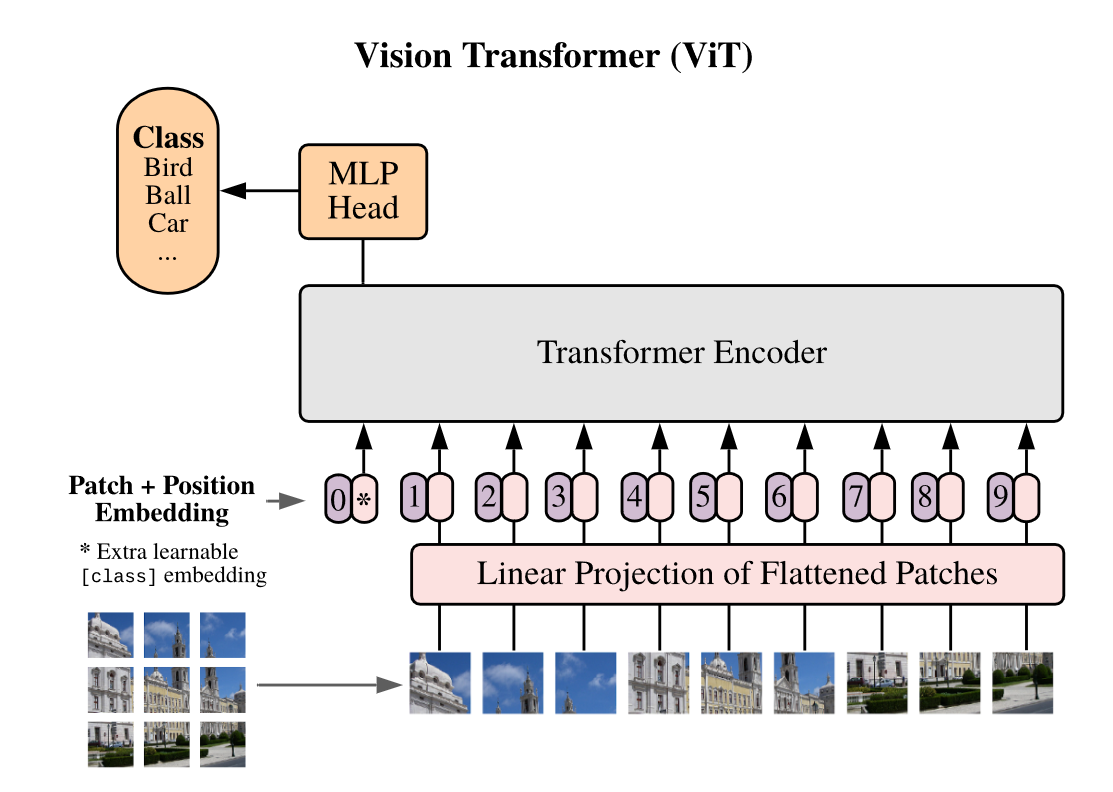
\includegraphics[scale=0.3]{vit.png}
	\caption{Архитектура Vision Transformers\cite{vit}.}
	\label{fig:vit}
\end{figure}

Архитектура Vision Transformers достигла высоких показателей производительности в задаче классификации изображений на датасете ImageNet после предварительного обучения на JFT-300M \cite{vit}. Однако важно отметить, что эффективность моделей резко снижается при использовании небольших объемов данных для предварительного обучения. Более крупные модели чаще всего показывают лучшие результаты на больших наборах данных. Это проблема, вероятно, связана с тем, что трансформерные сети не имеют предварительных предположений о порядке данных, что может привести к их недостаточной адаптации к конкретным требованиям задачи или к обучающему набору данных.



\subsection{Метрики качества в задаче классификации}\label{classification_metrics}
Одним из важных аспектов любой оптимизационной задачи является выбор метрик качества. Оценку качества классификационных моделей можно измерять многими способами, каждый из которых отражает различные стороны модели. Выбор основной метрики качества косвенно оказывает сильное влияние на конечный результат, поскольку при обучении модели с гиперпараметрами, их подбор производится с целью увеличения значения выбранной метрики качества. В свою очередь выбор метрики качества зависит от поставленной задачи, чаще всего зависящей от бизнес-целей, а также от особенностей данных, с которыми производится работа. Наиболее распространенными метриками качества для задачи классификации являются точность (англ. precision), полнота (англ. recall), F-мера (англ. F1-measure), ROC-AUC, индекс Джини и другие. Сперва некоторые из них будут рассмотрены с теоретической точки зрения. Затем в рамках задачи, поставленной в данной работе.

Наиболее простой в понимании является метрика accuracy\footnote{Во избежание путаницы с названием метрик качества на русском языке, поскольку некоторые из них имеют одинаковый перевод, в тексте будут использоваться их английский названия.} – доля правильных ответов:

\begin{equation}
	\label{acc}
	accuracy(a, X) = \frac{1}{n}\sum_{i=1}^{n}[a(x_i)=y_i],
\end{equation}
где a - алгоритм, X - объекты, n - кол-во объектов,	$a(x_i)$ - предсказание алгоритма на объекте $x_i$,	$y_i$ - истинные ответы. Однако из-за своей простоты accuracy имеет сильные недостатки и не походит в большинстве реальных задач. Наиболее серьезной проблемой является плохое отражение качества работы алгоритма при несбалансированных данных. Она абсолютно не учитывает дисбаланс классов. Например, в задаче диагностики редких заболеваний классификатор, предсказывающий всем пациентам отсутствие болезни будет иметь достаточно высокую accuracy просто потому, что больных людей в выборке намного меньше. Другим ее недостатком является то, что по ней нельзя сказать, в какую сторону ошибается алгоритм. Можно снова привести в пример задачу медицинской диагностики: в случае ошибочного положительного диагноза для здорового больного обернётся лишь ещё одним обследованием, то ошибочно отрицательный вердикт может повлечь роковые последствия. Разновидность обычной accuracy является метрика accuracy top-k, которая измеряет процент случаев, когда истинный класс присутствует среди верхних k предсказанных классов. Top-k accuracy полезна, когда интерес представляет не только самый вероятный предсказанный класс, но и его ближайшие альтернативы. Чаще всего рассчитывается accuracy@top2. В этом случае модель оценивается по тому, насколько точно она предсказывает правильный класс, если учитывать два наиболее вероятных класса (первый и второй по вероятности). Это означает, что если правильный класс присутствует среди первых двух предсказанных классов, то это считается успешным предсказанием.

Для расчета многих метрик используется матрица ошибок классификаций (англ. confusion matrix). Рассмотрим принцип ее построения на примере бинарной классификации и алгоритма, предсказывающего принадлежность каждого объекта одному из классов (см. таблицу \ref{confusion_matr}. Как правило, класс, представляющий интерес, называется «положительным» (в таблице - класс 1), а оставшийся – «отрицательным» (в таблице – класс 0). Вся матрица разделена на 4 части, отражающие возможные ситуации при предсказании. В верхнем левом квадрате (англ. true positive) находятся объекты, у которых был предсказан «положительный» класс, и он совпал с истинным. В противоположность в правом нижнем углу (англ. true negative) находятся объекты, у которых был предсказан «отрицательный» класс, который также совпал с истинным. На другой диагонали находятся так называемые «ошибки» модели. В нижнем левом углу помещаются объекты, которые алгоритм не смог опознать как «положительный» класс. В правом верхнем квадрате – объекты, которые алгоритм ошибочно отнес к «положительному» классу.

\begin{table}[h]
	\centering
	\begin{tabular}{ | l | l | l | }
		\hline
		& $y = 1$ & $y = 0$ \\ \hline
		$\hat{y} = 1$ & True Positive (TP) & False Positive (FP) \\ \hline
		$\hat{y} = 0$ & True Negative (TN) & False Negative (FN) \\ \hline
	\end{tabular}
	\caption{Матрица ошибок классификации.
		$y$ — истинный класс, $\hat{y}$ — результат модели.}
	\label{confusion_matr}
\end{table}

На матрице ошибок основываются такие метрики как precision, recall и их агрегация F1-мера: Precision (см. формулу \ref{precision}) отражает то, насколько можно доверять классификатору. Другими словами, это доля объектов, которые классификатор определил как положительные и при этом они действительно являются положительными. Введение precision не позволяет определять все объекты в один класс, так как в этом случае получается рост false positive объектов. Recall (см. формулу \ref{recall}) показывает, какую долю положительных объектов из всех объектов положительного класса обнаружила модель. Recall отражает способность метода вообще обнаруживать данный класс, а precision — способность отличать этот класс от других. В отличие от accuracy, recall и precision не зависят, от соотношения классов и поэтому могут быть применимы на несбалансированном датасете. Однако, используемые по отдельности, данные метрики не дают полного понимания картины. Если precision равен 1, то ложноположительные классификации отсутствуют. Однако это ничего не говорит о том, были ли распознаны все положительные примеры. Если же recall равен 1, то все положительные объекты были распознаны правильно, а ложноотрицательные классификации отсутствуют. При этом ничего не говорится о том, сколько было допущено ложноположительных классификаций.

\begin{equation}
	\label{precision}
	precision = \frac{TP}{TP + FP}
\end{equation}

\begin{equation}
	\label{recall}
	recall = \frac{TP}{TP + FN}
\end{equation}


Как уже было сказано ранее F1-мера объединяет precision и recall в своей оценки (см. формулу \ref{f1}). В базовом варианте F1-мера предполагает одинаковую важность precision и recall, однако если одна из этих метрик является более приоритетной, можно воспользоваться $\ F_\beta$ мерой.

\begin{equation}
	\label{f1}
	\large \ F_\beta = (1 + \beta^2) \cdot \frac{precision \cdot recall}{(\beta^2 \cdot precision) + recall}
\end{equation}

$\beta$ в данном случае определяет вес точности в метрике. 

Все вышеперечисленные метрики качества являются ограниченными сверху и снизу и располагаются в интервале [0, 1]. F1-мера достигает максимума при точности и полноте, равными 1, и близка к 0, если один из аргументов близок к 0. Данная особенность позволяет производить точное сравнение качества разных моделей классификации.

Другим семейством метрик в задаче классификации выступают интегральные метрики\footnote{Интегральная метрика качества – метрика, отражающая качество алгоритма, вне зависимости от выбранного порога.}. Данные метрики удобны тем, что она показывают качество классификатора независимо от выбранного порога. В классификационных моделях часто стоит вопрос о правилах отнесения объекта к положительному или отрицательному классу. Обычно для этого используется вероятностный порог. Из модели возвращается оценка вероятности принадлежности объекта к положительному классу и в зависимости от установленного порога объект будет отнесен к соответствующему классу. Для поставленной задачи будут интересны следующие интегральные метрики: ROC-curve, PR-curve, AUC и Average Precision. Рассмотрим подробнее каждую из них.

Наиболее интуитивным является порог, равный 0.5. Однако такой порог отсечения не всегда может являться оптимальным. При уменьшении порога отсечения будет находиться (правильно предсказываться) всё большее число положительных объектов, но также и неправильно предсказываться положительная метка на всё большем числе отрицательных объектов. Для этого были введены две метрики TPR (true positive rate) и FPR (false positive rate) (см формулу \ref{tpr-fpr}). TPR отражает долю неверно принятых объектов отрицательного класса, FPR – долю верно принятых объектов положительного класса.

\begin{equation}
	\label{tpr-fpr}
	TPR = \frac{TP}{TP + FN} \quad FPR = \frac{FP}{FP + TN} 
\end{equation}

В терминах TPR и FPR как раз и строится ROC-curve (см. рисунок \ref{fig:roccurve}). При идеальной классификации ROC кривая начинается в точке (0; 0), проходит через верхний левый (точка (0;1)) и заканчивается в правом верхнем углу (точка (1;1)). В случае случайной работы классификатора ROC кривая будет иметь диагональный вид, начинаясь в нижнем левом углу и заканчиваясь в правом верхнем.

\begin{figure}[ht]
	\centering
	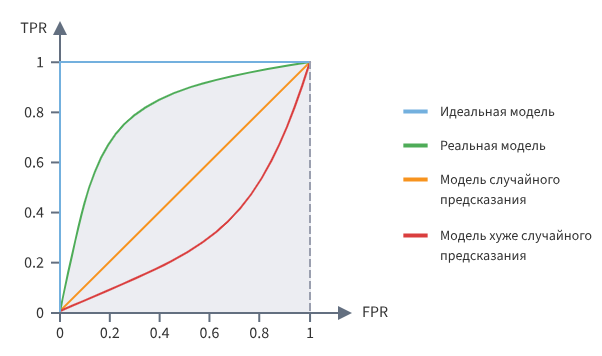
\includegraphics[scale=0.8]{roccurve.png}
	\caption{Пример построенной ROC кривой \cite{loginom}.}
	\label{fig:roccurve}
\end{figure}

Для более точного сравнения ROС кривых считают показатель AUC (Area Under the ROC Curve) – площадь под ROC кривой. Данная мера может принимать значения в диапазоне от 0 до 1, где 1 достигается при идеально классификации, а 0.5 соответствует случайной классификации. Метрика AUC довольно стабильна к дисбалансу классов, а также в целом показывает, насколько хорошо работает алгоритм.

Другой часто анализирующийся кривой является Precision-Recall кривая (PR-curve) (см. рисунок \ref{fig:prcurve}). В случае чересчур малой доли объектов положительного класса ROC-AUC может давать неадекватно хороший результат. PR-curve строится в терминах precision и recall, рассчитанных при разных порогах отсечения. Поскольку данная кривая строится в терминах precision-recall, которые устойчивы к дисбалансу классов, то и сама кривая более точно отражает качество модели при несбалансированных данных.

\begin{figure}[ht]
	\centering
	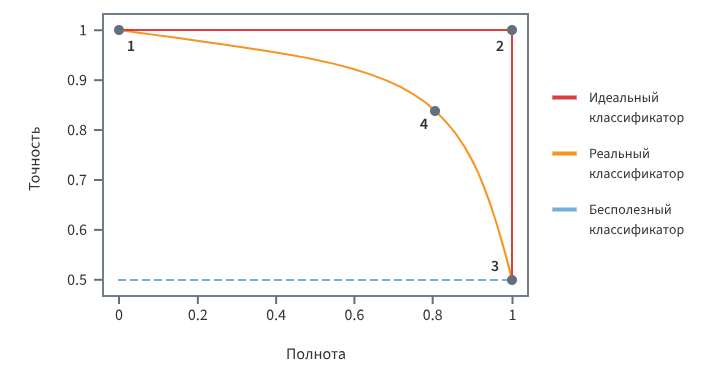
\includegraphics[scale=0.8]{prcurve.png}
	\caption{Пример построенной PR кривой \cite{loginom}.}
	\label{fig:prcurve}
\end{figure}

Аналогичной метрике AUC является метрика Average Precision (AP), отражающая площадь под PR кривой.

Все вышеупомянутые метрики рассматривалась в рамках задачи бинарной классификации. Однако в нашем случае решается задача многоклассовой классификации, поэтому необходима адаптация метрик. Существует 3 основных подхода к расчету метрик в многоклассовом случае: микроусреднение (англ. micro average), макроусреднение (англ. macro average) и взвешенное среднее (англ. weighted average). Идея всех подходов – сведение подсчета метрик к бинарному случаю.

При микроусреднении для каждого класса k в отдельности рассчитываются элемента матрицы ошибок ($TP_k$, $FP_k$, $TN_k$, $FN_k$). Затем полученные характеристики усредняются по всем классам (см. формулу \ref{micro-average}) и используются для расчета precision и recall.

\begin{equation}
	\label{micro-average}
	TP = \frac{1}{K}\sum_{k=1}^{K}TP_k
\end{equation}

В макроусреднении также для каждого класса k в отдельности рассчитываются элемента матрицы ошибок ($TP_k$, $FP_k$, $TN_k$, $FN_k$). Далее на основании полученных значений производится расчет $precision_k$ и $recall_k$ (см. формулу \ref{macro-average}). Затем происходит усреднение полученных характеристик по классам (см. формулу \ref{macro-average2}).

\begin{equation}
	\label{macro-average}
	precision_k(a, X) = \frac{TP_k}{TP_k + FP_k}
\end{equation}

\begin{equation}
	\label{macro-average2}
	precision(a, X) = \frac{1}{K}\sum_{k=1}^{K}precision_k(a, X)
\end{equation}

При взвешенном среднем происходит аналогичный расчет макроусреднению. С тем отличием, что в макроусреднении усреднение по классам происходило с равными весами, а в случае взвешенного среднего усреднение метрик, рассчитанных для каждого класса, происходит с весами, пропорциональными количеству объектов в классе.

Используя микроусреднение, уменьшается влияние малочисленных классов. При макроусреднении вклад каждого класса в финальную метрику будет одинаковым. Третий подход является неким компромиссом между первыми двумя.

Теперь перейдем к использованию метрик качеств в рамках данной работы. Проектируемый сервис исходит в первую очередь из бизнес-задачи. Разрабатывается функционал для улучшения ключевых метрик, таких как привлечение новых пользователей, конверсия и увеличения прибыли. предложив уникальные функции, которых нет у конкурентов, или те, которые превосходят конкурирующие решения. К сожалению, бизнес-задачи напрямую не всегда можно переложить в измеримые метрики. К таким целям как раз относится и увеличение прибыли компании, которая зависит от многих факторов и не подходит в качестве измерителя в задачах машинного обучения. Кроме того, оценить эффективность нового функционала возможно только спустя месяц, поскольку потребуется время для составления корректных отчетов по продажам, или по завершении сезона, когда продавцы, используя сервис, смогут подобрать наилучшую категорию товаров. Это, в свою очередь, может привести к росту продаж, что станет показателем успешности предложенных решений. Для этого удобно проведение A/B-тестирования, которое позволяет сравнивать результаты «с» и «без» использования нового функционала, а также получить точные данные о его влиянии на ключевые метрики.

Разобравшись с метриками, исходящих от бизнеса, и придя к заключению о невозможности их использования напрямую в данном проекте, стало крайне важным найти наиболее близко коррелируемые с данными показателями метрики машинного обучения. 

Поскольку данные, с которыми производится работа, имеют сильный дисбаланс классов, более подходящими метриками качества будут являться precision, recall и их обобщения. Стоит отметить, что в поставленной формулировке задачи достижение идеального качества не является обязательным условием, поскольку неточности модели могут быть обернуты в рамки взаимодействия с пользователем. Например, при неуверенной классификации можно попросить пользователя перезагрузить другую фотографию или попросить выбрать наиболее подходящую по его мнению категория из списка наиболее подходящих категорий по мнению модели. В данной работе для получения более обширной картины при построении и оптимизации классификационных моделей рассчитывались как интегральные, так и зависящие от выбранного порога метрики. В качестве неинтегральных метрики рассчитывались accuracy, precision, recall, f1. Из них наибольший интерес представляла метрика precision, поскольку цена неверно подобранной категории для объекта довольно высока. Другими словами, гораздо важнее получить уверенный классификатор, который будет допускать минимум ошибок при своей высокой уверенности в полученном результате. Также некоторый интерес представляла accuracy@top2. Она полезна в ситуацияи, когда уверенность в предсказании модели не настолько высока, чтобы рассматривать только самое вероятное предсказание. Поскольку работа происходит с реальными данными (все особенности собранных данных см. раздел \ref{subsection:datastep2}), с большой вероятностью могут быть изображения, на которых нельзя однозначно определить класс, или товары, которые могут быть отнесены к разным, но относительно похожим категориям. В таком случае top-2 accuracy позволит учесть эту неопределенность.

В отношении использовании микро и макроусреднений в поставленной задаче стоит отметить, что поскольку во всех моделях присутствует в разной степени дисбаланс классов, в макроусреднении при усреднении метрик малых и больших классов важность объектов малочисленных классов будет завышена. В альтернативном случае при микроусреднении плохие предсказания для малочисленных классов будут растворяться по общем фоне метрики, то есть их роль в финальном показателе будет преуменьшена. Исходя из целей работы и особенностей собранных данных, в разрабатываемой классификационной модели важно предсказывать правильно все классы, а не только наиболее большие и популярные. То есть при обучении классификационных моделей и анализе их качества ориентир будет направлен главным образом на метрики, полученные посредством макроусреднения.

Как уже было сказано ранее, на финальное предсказание модели можно повлиять с помощью выбранного вероятностного порога отсечения, согласно которому тот или иной объект будет или не будет относиться к положительному классу. В задачах с взаимодействием с пользователями такая настройка может сыграть решающую роль, поэтому для более грамотного принятия решения при получении предсказаний мы будем опираться на Precision-Recall кривую. При понижении порога отсечения модель большее число объектов будет попадать в положительный класс, то есть произойдет увеличение recall. При повышении вероятностного порога модель будет больше уверена в своих предсказания, однако шанс выявить все объекты положительного класса сократиться, то есть произойдет увеличение precision. Порог отсечения подбирался в каждом классификаторе индивидуально.

Также для полной картины для каждого классификатора были построены ROC кривые и рассчитаны AUC и Average Preсision.





















\subsection{Задача создания подписей к изображениям}\label{subsection:image-captioning}

Задача создания подписей к изображениям (от англ. image captioning) предполагает использование методов глубокого обучения для генерации текстовых описаний на основе визуального содержимого изображений. Для решения этой задачи используется архитектура кодера-декодера (от англ. encoder-decoder). Основные подходы для ее реализации:
\begin{enumerate}[label=\arabic*.]
	\item Использование комбинации сверточных нейронных сетей для обработки изображения и рекуррентных нейронных сетей для генерации подписи. 
	\item Использование трансформеров. 
\end{enumerate}

Архитектура с использованием комбинации CNN и RNN представлена на рисунке \ref{fig:image-caption-cnn-rnn}. В качестве кодировщика используется CNN, такие как ResNet, MobileNet или EfficientNet. Эти модели предварительно обучены на больших наборах данных, таких как ImageNet, для извлечения визуальных признаков. Кодировщик отвечает за преобразование изображения в компактное представление (вектор признаков), которое сохраняет важную информацию об изображении. В качестве вектора признаков изображения может использоваться выходной слой CNN, но чаще всего это слой перед последним полносвязанным. Декодировщик принимает вектор признаков изображения и генерирует последовательность слов, которая описывает изображение. Декодеры, как правило, основаны на рекуррентных нейронных сетях (RNN), такие как LSTM (Long Short-Term Memory) или GRU (Gated Recurrent Unit). Одна из основных проблем такого подхода — это то, что RNN имеет фиксированную длину контекста и обрабатывает информацию последовательно. Это означает, что RNN видит только небольшой контекст, поэтому при генерации слов часто забывает старые результаты своей генерации. Так же такой подход не позволяет полностью учесть контекст изображения на каждом этапе генерации. В данном случае выделенные признаки изображения с помощью CNN лишь единожды подаются на вход LSTM блока, так что со временем генерация полностью теряет память о исходном изображении и начинает «додумывать самостоятельно». Для решения этих проблем применяется механизм внимания (от англ. attention)\cite{attention}, основная идея которого состоит в том, чтобы позволить модели обрабатывать входные данные, учитывая их важность и относительные взаимосвязи между элементами данных. Это позволяет модели более гибко и точно адаптироваться к различным задачам и условиям входных данных, улучшая качество и эффективность моделирования. Механизм внимания может быть реализован разными способами:
\begin{itemize}
	\item В классической реализации RNN cкрытый вектор объединяет в себе информацию, содержащуюся в векторах вывода текущей итерации, через среднее или суммирование, которое можно заменить определенным взвешиванием всех предыдущих векторов, участвующих в усреднении, т.е для получения k-го скрытого вектора производится взвешивание k-1 предыдущего вектора. Веса при этом подбираются в зависимости от важности того или иного слова, что позволяет модели сосредотачивать внимание на различных аспектах входных данных в соответствии с контекстом задачи.
	\item Механизм внимания может быть интегрирован для учета контекста изображения при генерации каждого слова в описании. В этом случае кодер обрабатывает входное изображение с тремя цветовых канала, и преобразует его в изображение меньшего размера с «обученными» каналами. Это уменьшенное изображение представляет собой сводное представление всех полезных данных из исходного изображения. Механизм внимания использует это закодированное изображение, что позволяет сети «обращаться» к различным частям изображения на каждом шаге генерации текста. Весь этот процесс можно интерпретировать как вычисление вероятности того, что пиксел является важным для генерации следующего слова (см. рисунок \ref{fig:image-caption-decoder-att}). Таким образом, контекст самого изображения не теряется в процессе генерации текста. Механизм внимания позволяет сети фокусироваться на разных частях изображения с различной степенью «важности» на каждом этапе генерации, что значительно улучшает качество финального описания. На рисунке \ref{fig:image-caption-decoder-rnn} представлена архитектура декодера RNN с использованием механизма внимания на части изображения.
\end{itemize}

\begin{figure}[ht]
	\centering
	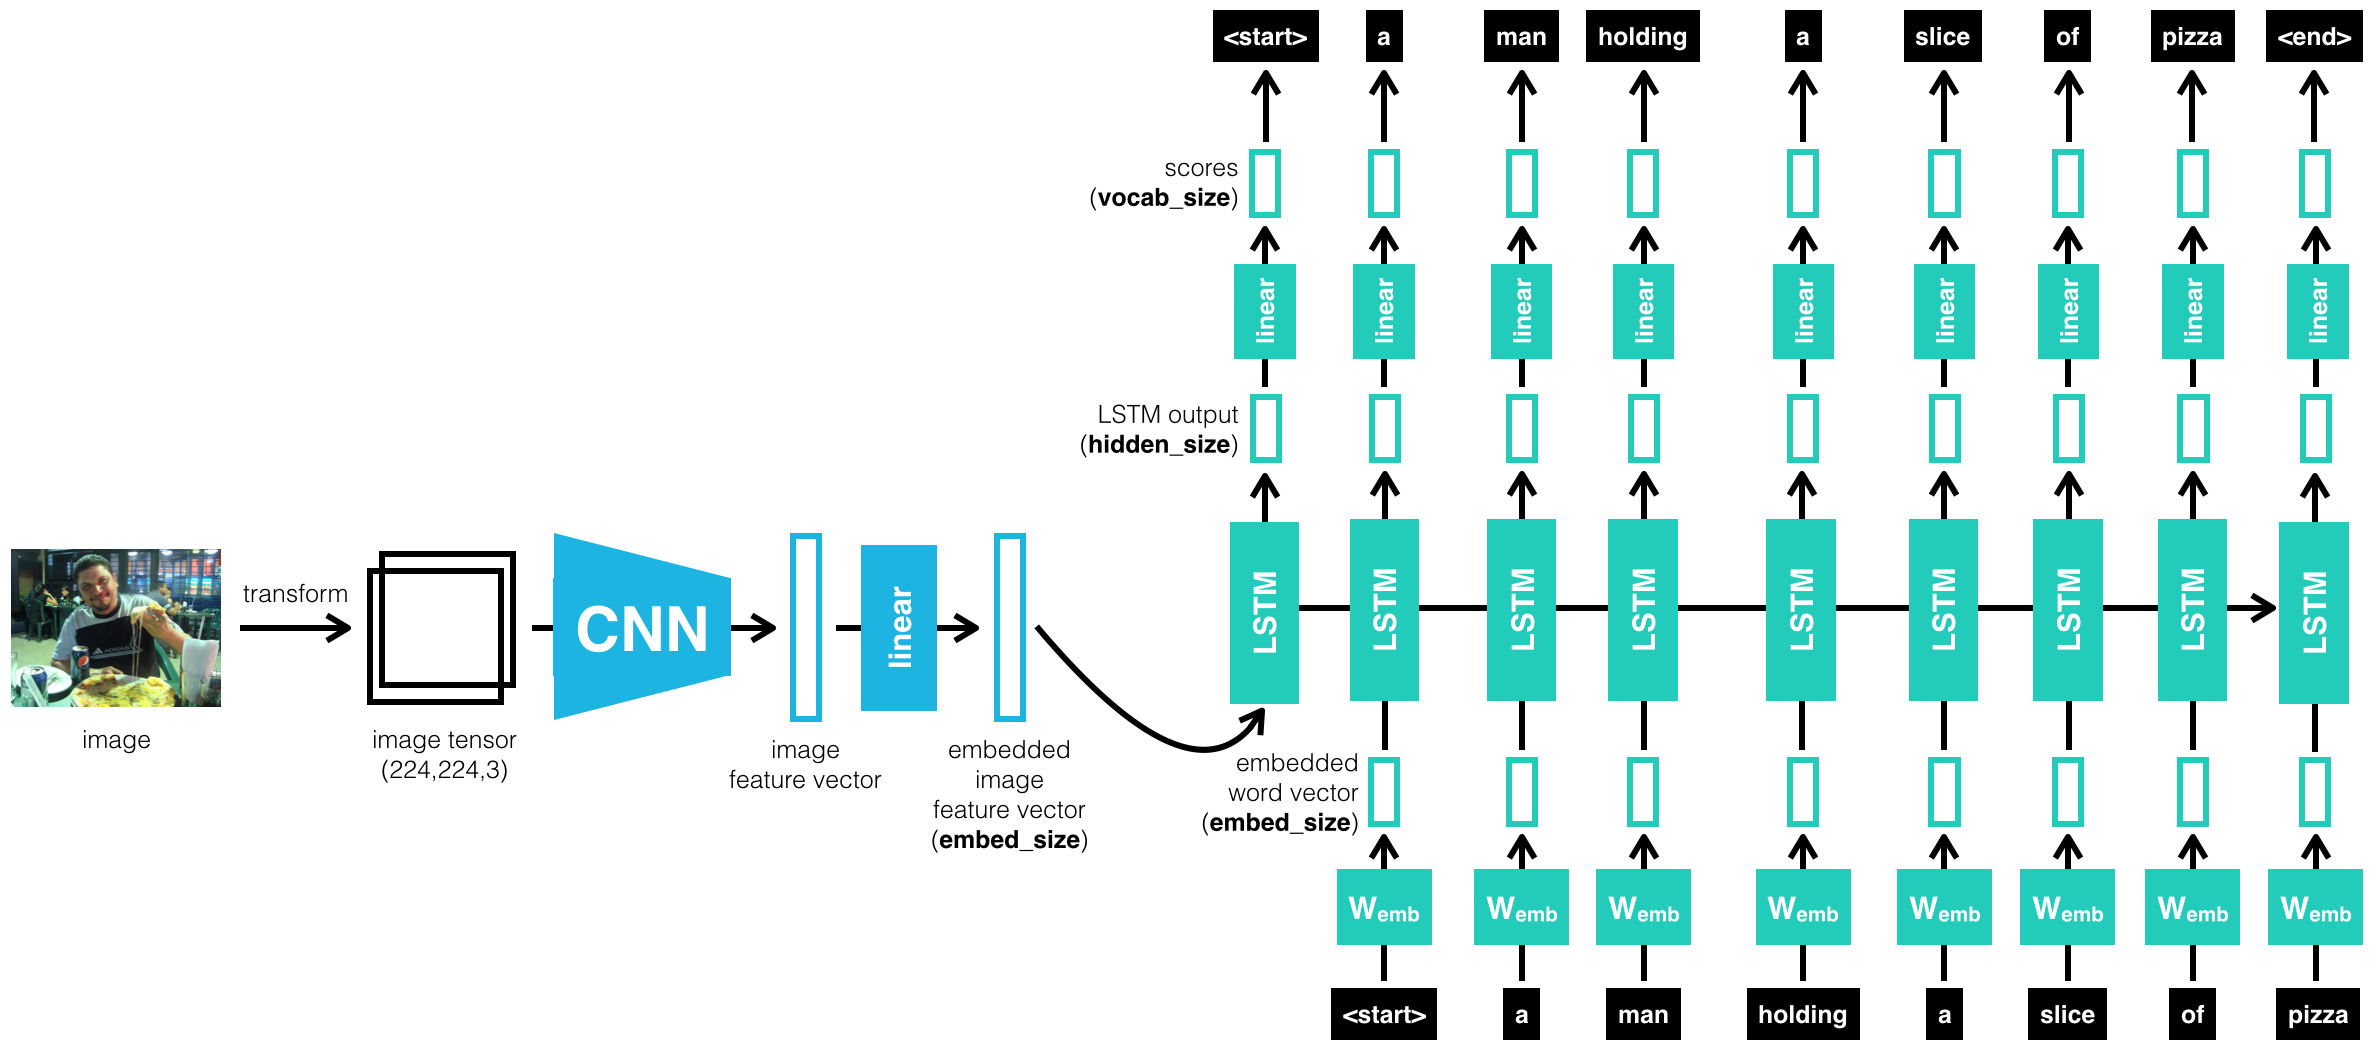
\includegraphics[scale=0.2]{image-captioning-cnn-rnn.png}
	\caption{Архитектура задачи Image Captioning c использованием комбинации CNN для обработки изображения и RNN для генерации подписи \cite{arch-cnn-rnn-image-captioning}.}
	\label{fig:image-caption-cnn-rnn}
\end{figure}

\begin{figure}[ht]
	\centering
	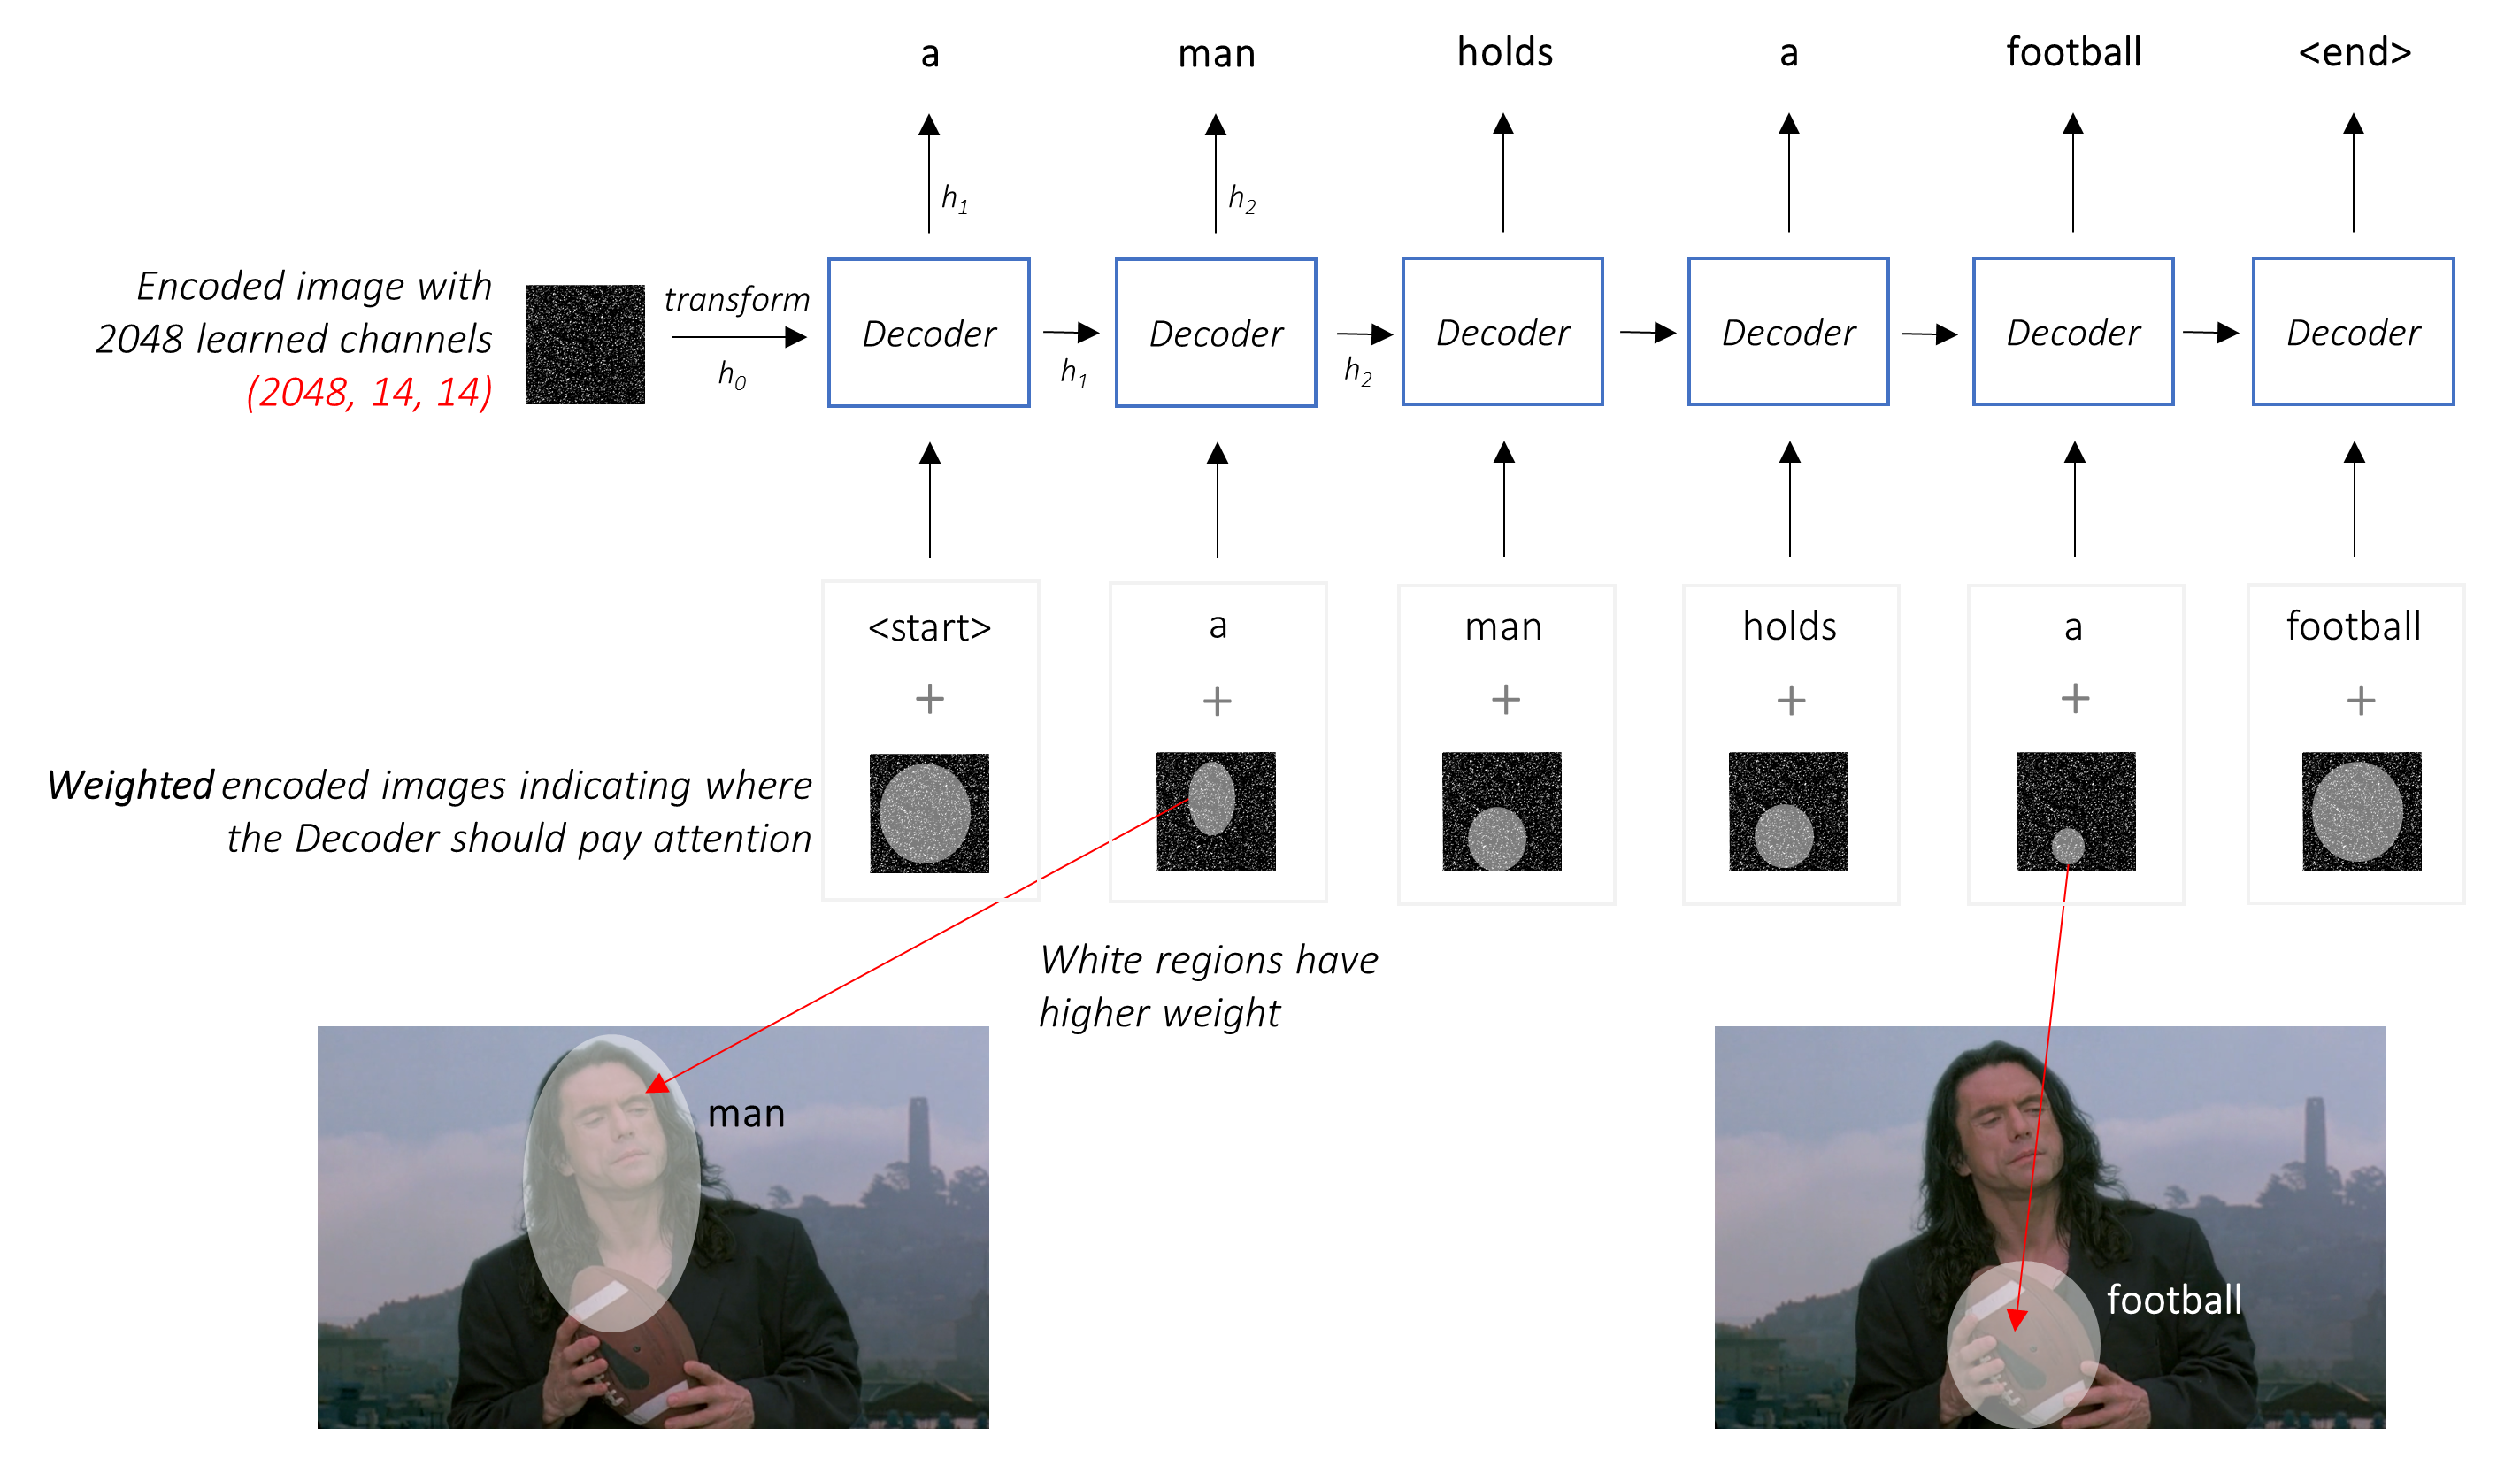
\includegraphics[scale=0.5]{decoder_att.png}
	\caption{Генерации последовательности с использованием механизма внимания на части изображения в задаче Image Captioning \cite{cnn-rnn-image-captioning}.}
	\label{fig:image-caption-decoder-att}
\end{figure}

\begin{figure}[ht]
	\centering
	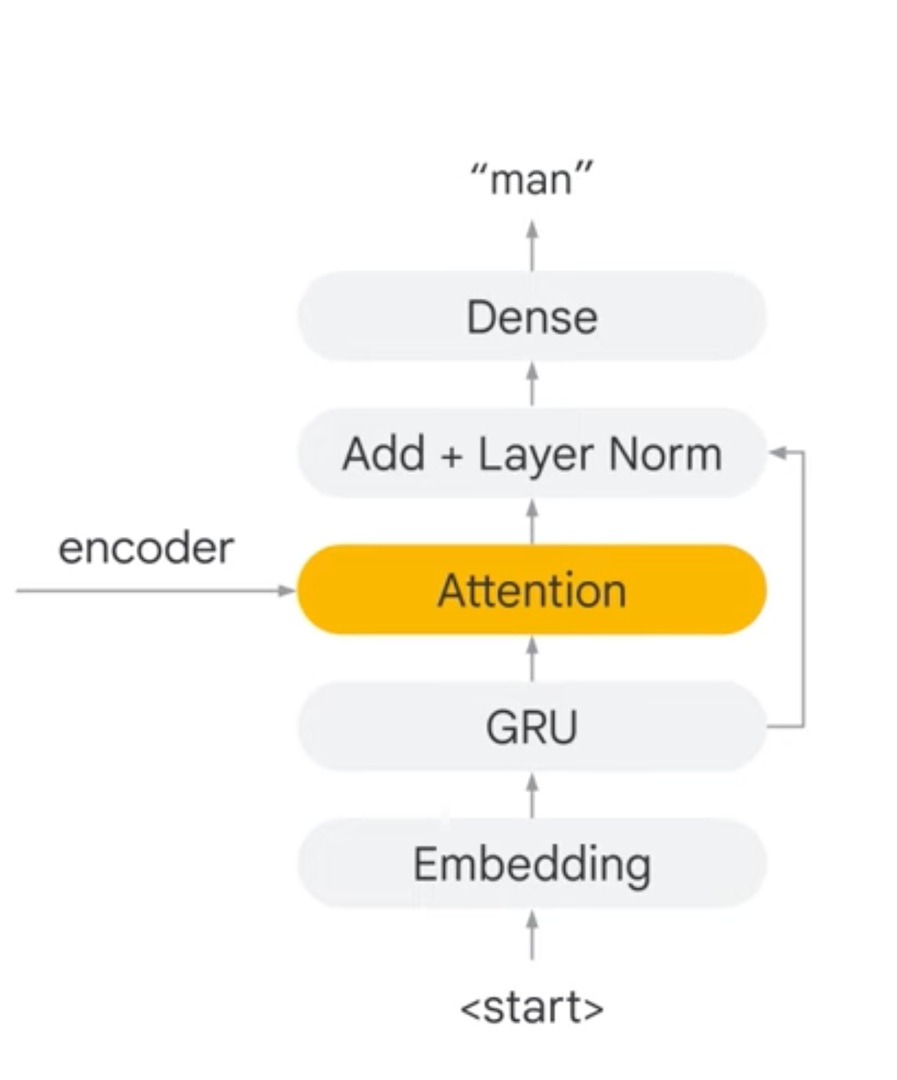
\includegraphics[scale=0.3]{image-captioning-decoder.png}
	\caption{Архитектура декодера RNN с использованием механизма внимания на части изображения в задаче Image Captioning \cite{cnn-rnn-image-captioning-google}.}
	\label{fig:image-caption-decoder-rnn}
\end{figure}

Преимущества реализации архитектуры с использованием комбинации CNN и RNN:
\begin{itemize}
	\item CNN позволяет эффективно и точно выделять особенности изображения, что обеспечивает богатую информацию для генерации текста; 
	\item модели CNN + RNN можно легко адаптировать и дообучать для различных задач и наборов данных.
\end{itemize}

К недостатком данной архитектуры можно отнести следующее:
\begin{itemize}
	\item Несмотря на улучшения в виде LSTM и GRU, RNN могут испытывать трудности с моделированием длинных текстов, что может влиять на качество генерации. 
	\item RNN могут генерировать текст, который не всегда полностью согласован с изображением. Иногда описание может быть частично правильным, но при этом не охватывать все важные детали изображения.
\end{itemize}


Архитектура  с использованием трансформеров представлена на рисунке \ref{fig:image-caption-transformers}. В качестве кодера используется Vision Transformers (ViTs), который применяет механизмы самовнимания к патчам изображения для извлечения признаков. В качестве декодера используются модели GPT, которые также используют механизмы самовнимания для моделирования долгосрочных зависимостей в тексте, что позволяет генерировать более связные и правильные описания. Ключевым моментом является правильная подача признаков изображения, извлеченных из ViTs, в соответствующие слои самовнимания GPT, то есть преобразование этих признаков в формат ключей (keys), значений (values) и запросов (queries).

\begin{figure}[ht]
	\centering
	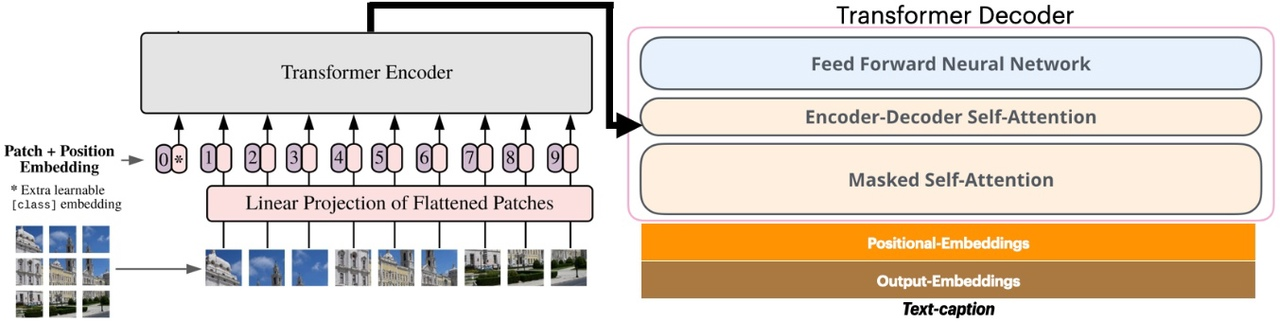
\includegraphics[scale=0.35]{image-caption-transformers.png}
	\caption{Архитектура задачи Image Captioning с использованием трансформеров \cite{vit-gpt2-image-captioning}.}
	\label{fig:image-caption-transformers}
\end{figure}

Преимущества реализации:
\begin{itemize}
	\item способность обрабатывать большие объемы данных и извлекать сложные зависимости.
	\item модели GPT обладают высоким качеством генерации текста благодаря своему предобучению на огромных объемах текстовых данных. Они способны генерировать разнообразные и грамматически правильные описания для изображений.
\end{itemize}

К недостатком данной архитектуры можно отнести то, что обучение моделей ViTs и GPT требует значительных вычислительных ресурсов и времени из-за их огромного размера и сложности.

Стоит отметить, что совместить способы решения задачи нельзя, из-за фундаментальных различий в их архитектурных подходах и методах обработки данных. CNN и RNN работают на основе последовательной обработки данных, в то время как ViTs и GPT используют механизмы самовнимания, которые позволяют параллельно обрабатывать данные. Комбинация подходов может потребовать значительных изменений в архитектурах, что вряд ли приведет к улучшению результатов. Поэтому выбор архитектуры (CNN + RNN или ViT + GPT) зависит от конкретных требований проекта и условий, в которых будет использоваться модель. В некоторых случаях может быть полезным попробовать обе архитектуры и выбрать ту, которая лучше соответствует задачам и ресурсам.

\subsection{Обзор моделей для генерации текста}

В данном разделе рассматриваются ключевые модели генерации текста, их архитектурные особенности, а также преимущества и недостатки.

\subsubsection{Рекуррентные нейронные сети}

Рекуррентные нейронные сети (от англ. Recurrent Neural Networks, RNN) — это класс нейронных сетей, специально разработанных для обработки последовательных данных. RNN широко применяются в задачах, где порядок и зависимость данных во времени играют важную роль, например, в таких как обработка текста и генерация последовательностей.

RNN способны учитывать временные зависимости в данных, обрабатывая последовательности входных сигналов. Это достигается благодаря наличию скрытых состояний (hidden states), которые обновляются на каждом шаге последовательности и хранят информацию о предыдущих шагах. В отличие от обычных нейронных сетей, RNN имеют петли обратной связи, позволяющие информации циркулировать внутри сети. Это позволяет RNN «помнить» предыдущие шаги и использовать эту информацию для текущих вычислений (см. рисунок \ref{fig:rnn_arch}).

\begin{figure}[ht]
	\centering
	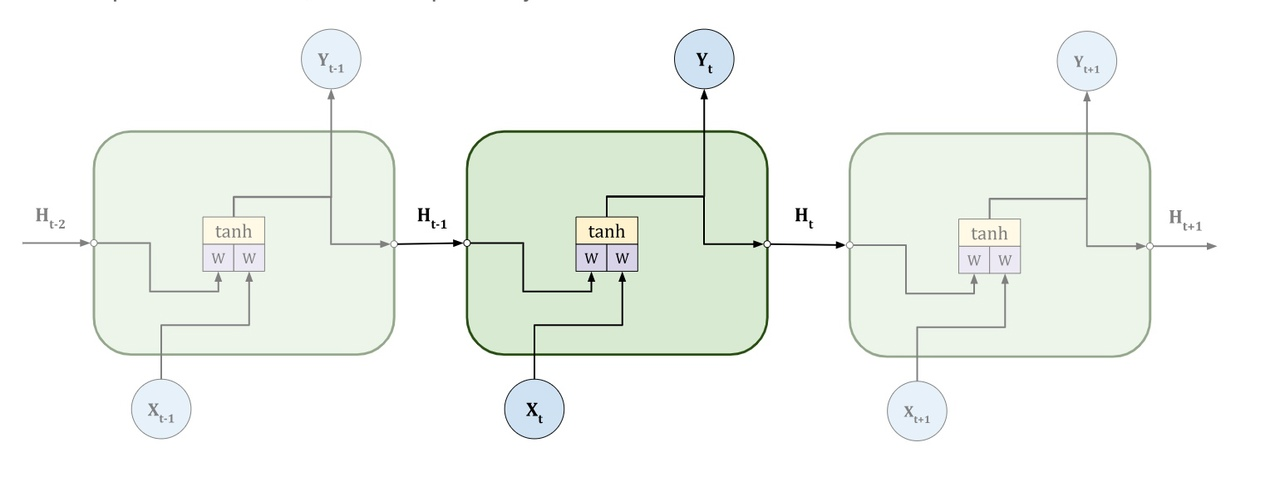
\includegraphics[scale=0.3]{rnn_arch.png}
	\caption{Архитектура RNN.}
	\label{fig:rnn_arch}
\end{figure}

На каждом шаге \( t \) входной вектор \( x_t \) и предыдущее скрытое состояние \( h_{t-1} \) используются для вычисления текущего скрытого состояния \( h_t \):
\begin{equation}
	\label{rnn_hidden_layer}
	h_t = \tanh(W_h h_{t-1} + W_x x_t + b_h)
\end{equation}
где \( W_h \) и \( W_x \) — веса, \( b_h \) — смещение, и \( \tanh \) — активационная функция.

При обучении очень длинных последовательностей RNN могут столкнуться с проблемой затухания или взрыва градиентов. Это приводит к тому, что веса либо становятся очень маленькими, либо слишком большими, что затрудняет обучение. 

Для решения проблем затухания и взрыва градиентов были предложены более сложные архитектуры, такие как Long Short-Term Memory (LSTM) и Gated Recurrent Unit (GRU).

LSTM — это разновидность RNN, специально разработанная для борьбы с проблемой затухания градиентов. LSTM используют специальные ячейки памяти и механизмы управления потоком информации, что позволяет им эффективно хранить и обрабатывать данные с долгосрочными зависимостями, что является недостижимым для классических RNN.

Ячейка LSTM состоит из трех основных компонентов:
\begin{enumerate}[label=\arabic*.]
	\item Ворота забывания (от англ. Forget Gate), которые используются для управления продолжительностью памяти в ячейке, решая, какую информацию следует забыть, а какую сохранить:
	\begin{equation}
		\label{rnn_hidden_layer}
		f_t = \sigma(W_f [h_{t-1}, x_t] + b_f)
	\end{equation}
	где \( f_t \) — значение ворот забывания, \( W_f \) и \( b_f \) — веса и смещения для ворот забывания.
	
	\item Ворота ввода (от англ. Input Gate), которые определяют, какая часть новой информации должна быть сохранена в долгосрочной памяти ячейки LSTM. Они не только фильтруют входные данные, но и решают, какая информация достаточно важна для сохранения:
	\begin{align}
		i_t &= \sigma(W_i [h_{t-1}, x_t] + b_i) \\
		\tilde{C}_t &= \tanh(W_C [h_{t-1}, x_t] + b_C)
	\end{align}
	где \( i_t \) — значение входного ворота, \( W_i \) и \( b_i \) — веса и смещения для входного ворота, \( \tilde{C}_t \) — кандидат на обновление состояния.
	
	\item Ворота вывода (от англ. Output Gate), которые определяют, какая информация из текущего состояния ячейки будет передана в выходной сигнал сети.
	\begin{align}
		o_t &= \sigma(W_o [h_{t-1}, x_t] + b_o) \\
		h_t &= o_t \cdot \tanh(C_t)
	\end{align}
	где \( o_t \) — значение выходного ворота, \( W_o \) и \( b_o \) — веса и смещения для выходного ворота, \( h_t \) — скрытое состояние на текущем шаге, \( C_t \) — обновленное состояние ячейки.
\end{enumerate}

Комбинируя результаты всех трех ворот, LSTM обновляет состояние ячейки и скрытое состояние следующим образом:
\begin{enumerate}[label=\arabic*.]
	\item Обновление состояния ячейки:
	\begin{align}
	 	C_t &= f_t \cdot C_{t-1} + i_t \cdot \tilde{C}_t
	\end{align}
	\item Обновление скрытого состояния:
	\begin{align}
		h_t &= o_t \cdot \tanh(C_t)
	\end{align}
\end{enumerate}

Архитектура ячейки LSTM представлена на рисунке \ref{fig:lstm_arch}.

\begin{figure}[ht]
	\centering
	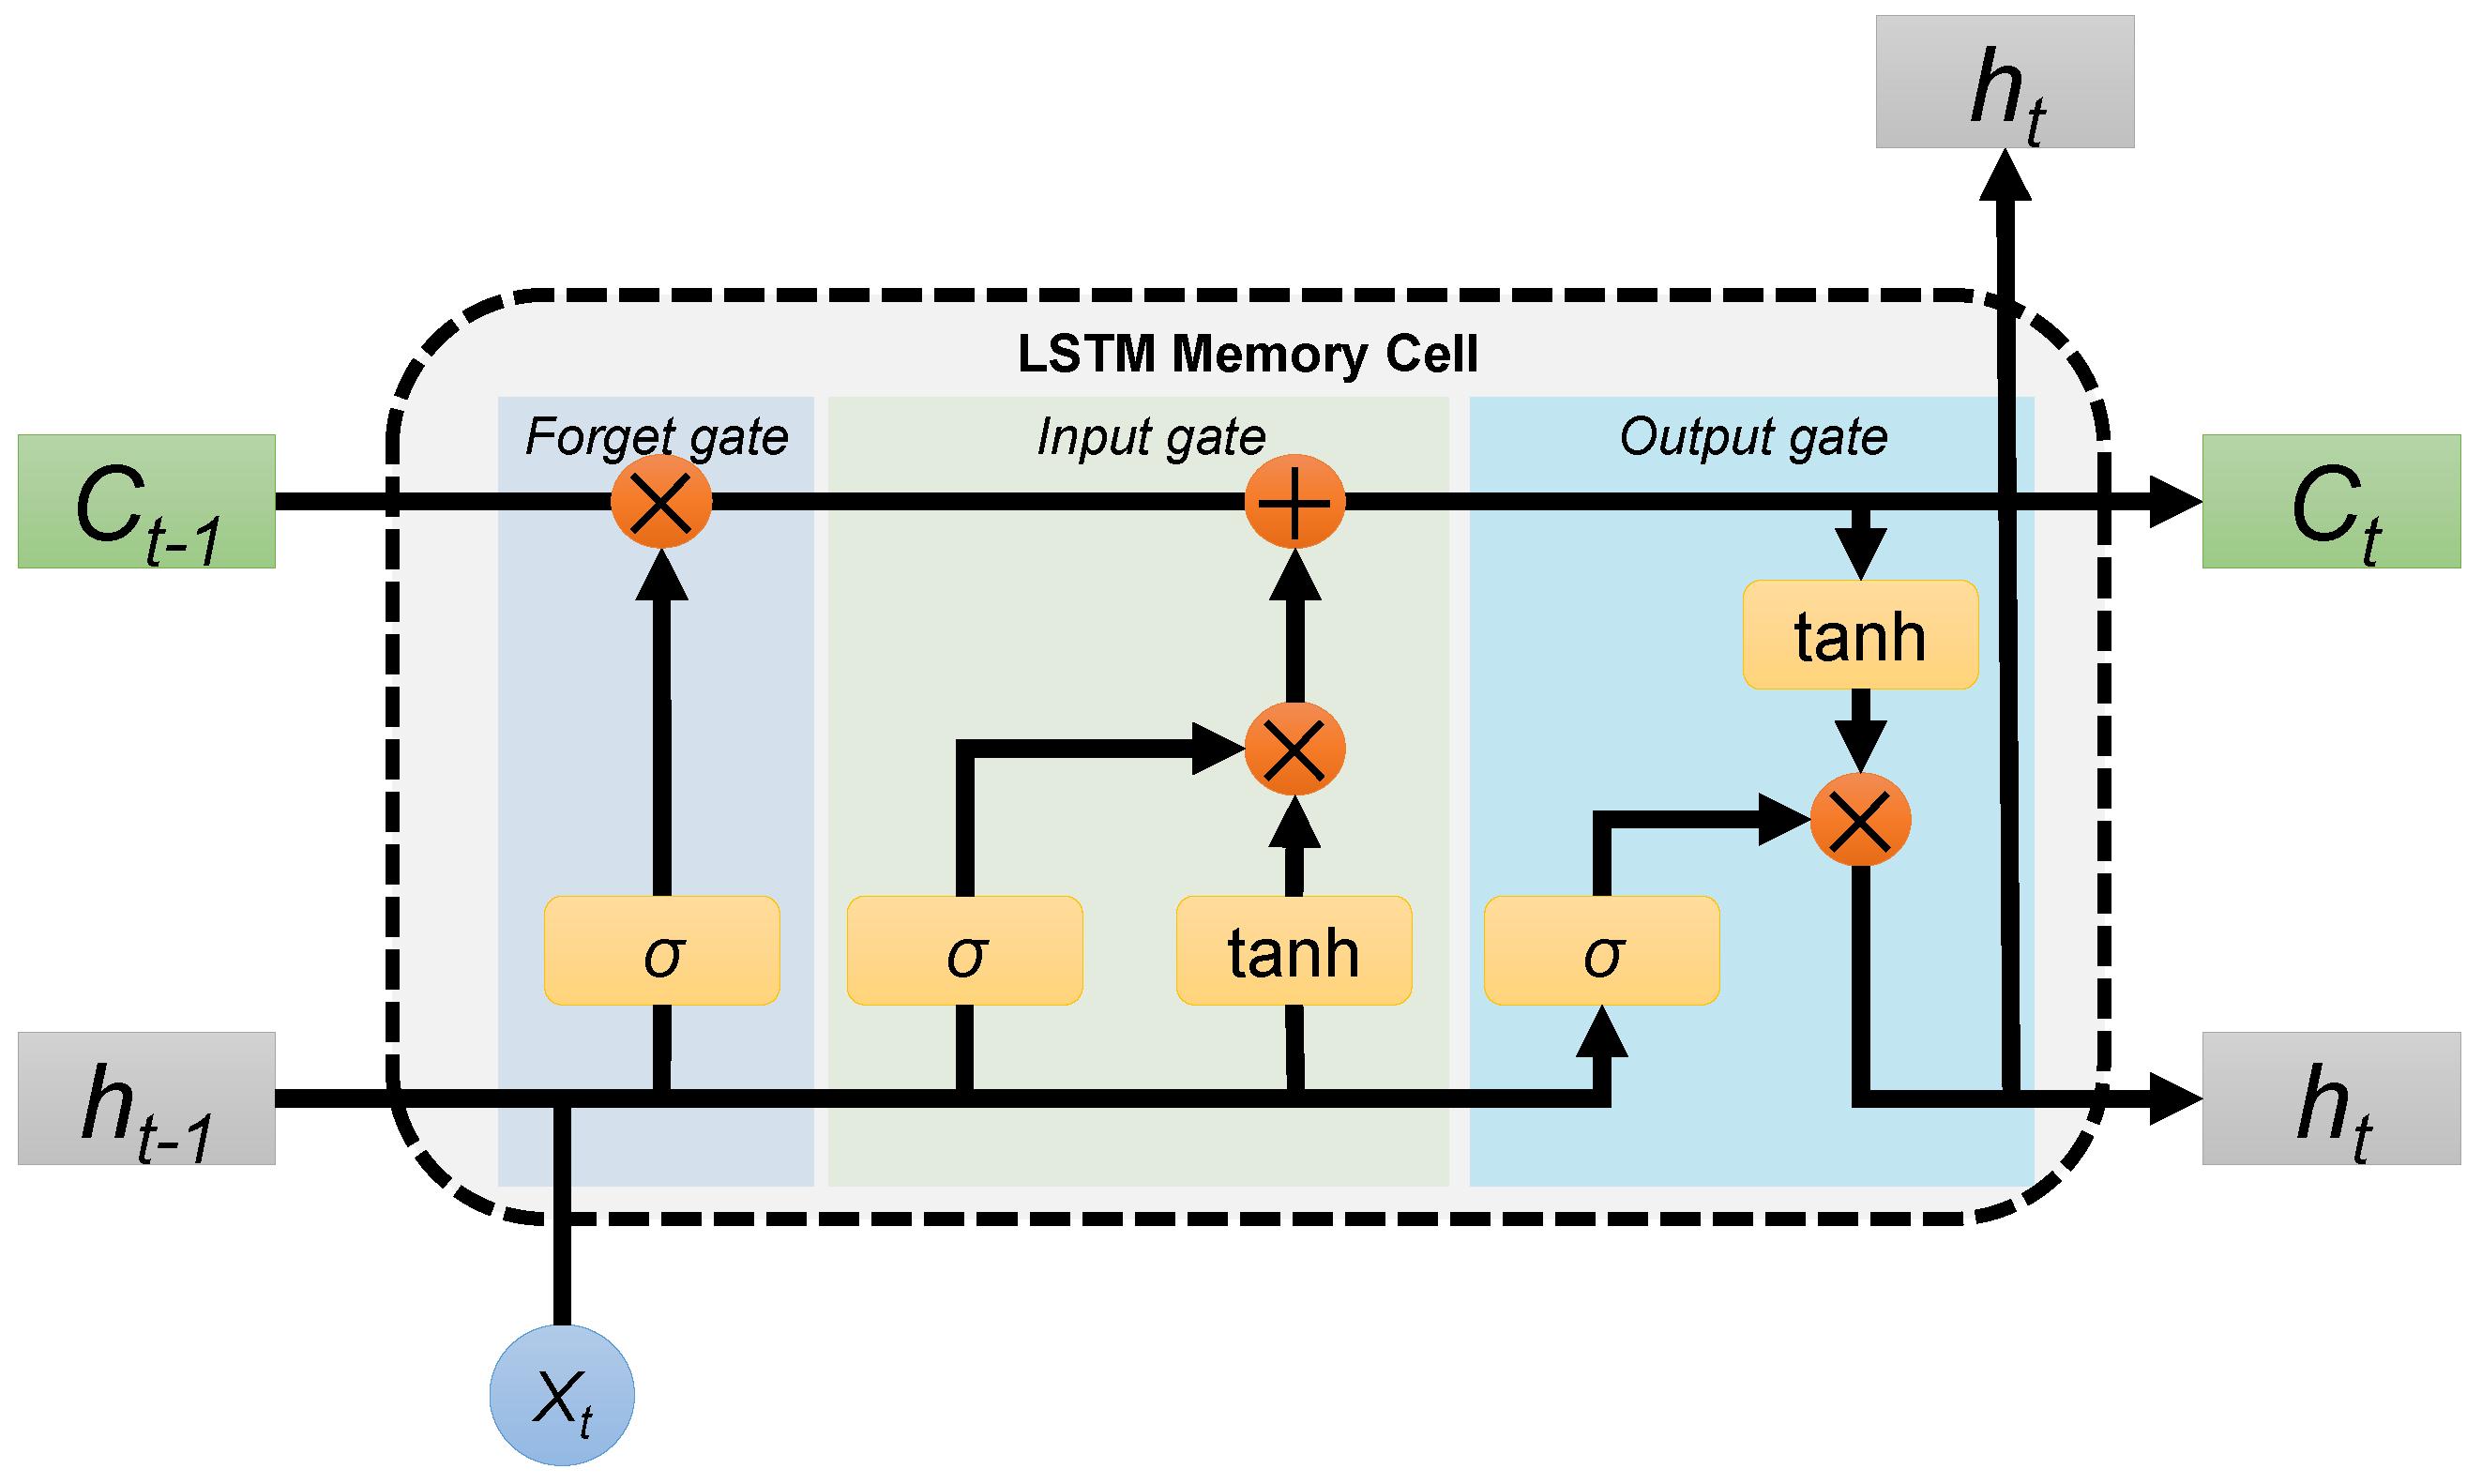
\includegraphics[scale=0.1]{lstm-cell.png}
	\caption{Архитектура ячейки LSTM.}
	\label{fig:lstm_arch}
\end{figure}


GRU — это упрощенная версия LSTM, которая объединяет забывающие и входные ворота в одно целое, что делает архитектуру менее вычислительно затратной и более простой для реализации. В GRU отсутствует отдельная ячейка памяти, характерная для LSTM. Вместо этого, скрытое состояние обновляется напрямую. Ворота обновления позволяют модели определить, какую часть предыдущего скрытого состояния следует сохранить, комбинируя его с новой информацией.

GRU использует два основных компонента:
\begin{enumerate}[label=\arabic*.]
	\item Ворота обновления (от англ. Update Gate), которые контролируют какая часть предыдущего скрытого состояния будет перенесена в текущее скрытое состояние.
	\begin{equation}
		z_t = \sigma(W_z \cdot [h_{t-1}, x_t] + b_z)
	\end{equation}
	где \( z_t \) — значение обновляющего ворот, \( W_z \) и \( b_z \) — веса и смещения для обновляющего ворот.
	\item Ворота сброса (от англ. Reset Gate), которые определяют какая часть предыдущего скрытого состояния будет сброшена перед вычислением нового состояния.
	\begin{equation}
		r_t = \sigma(W_r \cdot [h_{t-1}, x_t] + b_r)
	\end{equation}
	где \( r_t \) — значение сбрасывающего ворот, \( W_r \) и \( b_r \) — веса и смещения для сбрасывающего ворот.
\end{enumerate}


Новое скрытое состояние вычисляется с учетом текущего ввода и предыдущего скрытого состояния, модулированного сбрасывающими воротами. Формула для кандидата на новое скрытое состояние:
\begin{equation}
	\tilde{h}_t = \tanh(W_h \cdot [r_t \odot h_{t-1}, x_t] + b_h)
\end{equation}
где \( \tilde{h}_t \) — кандидат на новое скрытое состояние, \( \odot \) обозначает поэлементное умножение.


Итоговое скрытое состояние вычисляется как взвешенная сумма предыдущего скрытого состояния и кандидата на новое скрытое состояние, где веса задаются обновляющими воротами:
\begin{equation}
	h_t = (1 - z_t) \odot h_{t-1} + z_t \odot \tilde{h}_t
\end{equation}
где \( h_t \) — новое скрытое состояние, \( z_t \) — значение обновляющих ворот.

Архитектура ячейки GRU представлена на рисунке \ref{fig:gru_arch}.

\begin{figure}[ht]
	\centering
	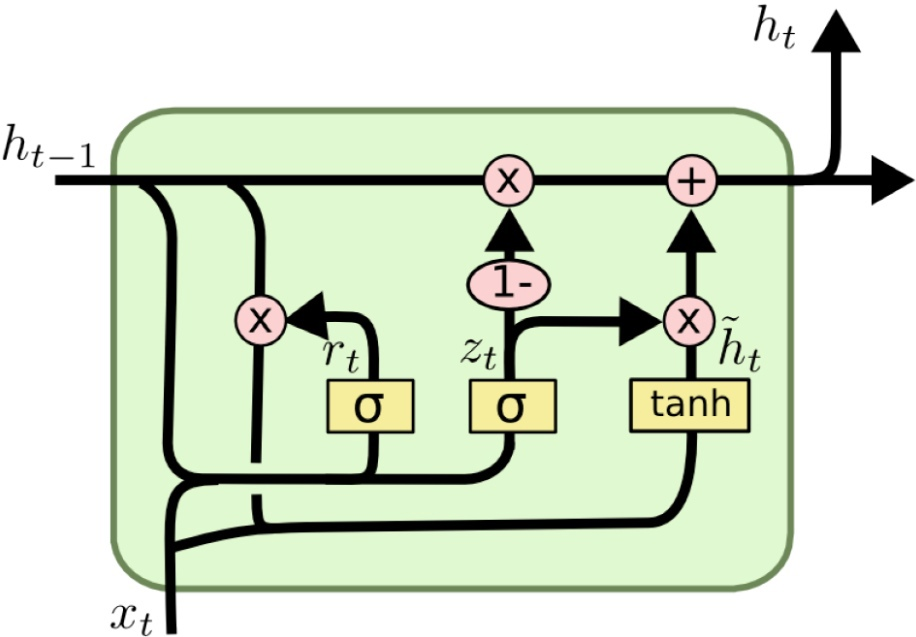
\includegraphics[scale=0.3]{gru-cell.png}
	\caption{Архитектура ячейки GRU.}
	\label{fig:gru_arch}
\end{figure}

Выбор между LSTM и GRU зависит от требований конкретной задачи. Если приоритетом является скорость обучения, а также ограничены вычислительные ресурсы, то GRU может оказаться предпочтительнее из-за своей более простой структуры и меньшего количества параметров. GRU также подходит для простых задач или небольших наборов данных, так как эффективно обучается без потери производительности. Однако, для задач, требующих детального управления информацией и долгосрочной памяти, например, в сложных задачах обработки естественного языка с длинными зависимостями, LSTM может быть более подходящим благодаря своей дополнительной сложности и улучшенному контролю над информацией.

\subsubsection{Модели генеративного предварительно обученного трансформера}

Модели генеративного предварительно обученного трансформера, (англ. Generative Pre-trained Transformer, GPT) — это семейство языковых моделей на основе глубокого обучения, разработанные командой OpenAI \cite{gpt-1}, которые используют архитектуру трансформера (см. рисунок \ref{fig:transformers_arch}) для генерации текста, учитывая контекст и структуру предложений. Модели GPT являются мощными инструментами для генерации текста и решения разнообразных задач в области естественного языка. Их успешное функционирование основано на комбинации трансформерной архитектуры, предварительного обучения на больших объемах текстовых данных и тщательного дообучения на конкретной задаче.

\begin{figure}[ht]
	\centering
	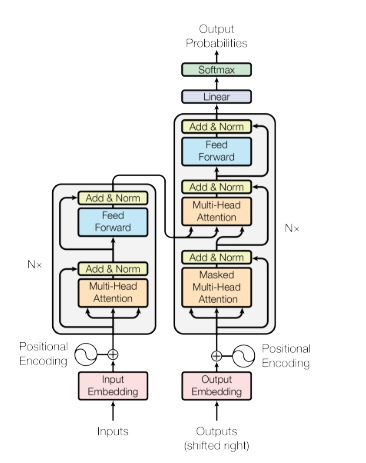
\includegraphics[scale=0.7]{transformer.png}
	\caption{Архитектура трансформера \cite{transformers}.}
	\label{fig:transformers_arch}
\end{figure}

Архитектура GPT имеет два основных сегмента: кодировщик, который в основном работает с входной последовательностью, и декодер, который работает с целевой последовательностью во время обучения и предсказывает следующий элемент.  Кодер определяет, какие части ввода следует выделить. Затем он вычисляет матрицу встраивания (встраивание в NLP позволяет словам с похожим значением иметь одинаковое представление) и преобразует ее в серию векторов внимания. Модели  GPT используют многоголовое внимание (от англ. multi-head attention), которое создает векторы внимания, позволяя модели одновременно фокусироваться на разных частях последовательности. Это позволяет захватывать различные аспекты контекста языка. Созданные вектора внимания проходят через слой нормализации и затем передаются в полносвязный слой. Нормализация помогает стабилизировать и ускорить процесс обучения. Перед передачей в декодер снова выполняется нормализация. Во время обучения кодер работает непосредственно с целевой выходной последовательностью.  Декодер вычисляет отдельные векторы встраивания для каждого слова предложения. Поскольку трансформеры не имеют встроенной последовательности обработки данных, то дополнительно применяется позиционный энкодер с синусоидальными и косинусоидальными функциями. Кроме того, модель GPT обучается предсказывать следующий токен в последовательности. Для этого используется механизм маскированного внимания (от англ. masked attention), который позволяет модели видеть только предшествующие токены. Во время генерации текста модель принимает на вход начальный токен или последовательность токенов и последовательно предсказывает следующие токены, генерируя текст по одному слову за раз. Процесс генерации продолжается до достижения определенного критерия остановки, например, такого как достижение максимальной длины текста или специального токена окончания.

Прежде чем приступить к выполнению конкретной задачи, модели GPT проходят через фазу предварительного обучения на больших корпусах текстовых данных. Во время предварительного обучения модель учится «понимать» структуру и смысл текста, а также создавать внутреннее представление о языке. После предварительного обучения модель может быть дообучена или донастроена на конкретной задаче, что улучшает ее производительность и качество результатов.


На данный момент существует несколько версий GPT, каждая из которых приносит свои улучшения и оптимизации:
\begin{enumerate}[label=\arabic*.]
	\item GPT-1 — первая модель из семейства GPT, которая содержит 117 миллионов параметров \cite{gpt-1}. Сложность обучения GPT-1 варьируется в зависимости от доступных вычислительных ресурсов и объема данных для обучения, но в то же время остается доступной для исследователей и специалистов благодаря наличию предобученных моделей. 
	\item GPT-2 содержит 1.5 миллиарда параметров. Обучение GPT-2 требует больших объемов данных и вычислительных ресурсов, что делает его более сложным в обучении, чем GPT-1 \cite{gpt-2}. Для многих исследовательских групп доступ к достаточным ресурсам может быть препятствием для обучения GPT-2, хотя предобученные модели могут быть доступны для использования.
	\item GPT-3 содержит 175 миллиардов параметров \cite{gpt-3}. Обучение GPT-3 требует огромных вычислительных ресурсов и больших объемов данных, что делает его крайне сложным в обучении. Для большинства исследовательских групп доступ к таким ресурсам может быть недостижимым. Кроме того, обучение GPT-3 может требовать значительных финансовых затрат на инфраструктуру и вычислительные ресурсы.
	\item GPT-4 — мультимодальная большая языковая модель, которая способна обрабатывать запросы в виде картинок и текста, а затем выдавать текстовые ответы. В качестве трансформера GPT-4 была предварительно обучена прогнозировать следующий токен (используя как общедоступные данные, так и «данные, лицензированные сторонними поставщиками»), а затем была доработана с помощью обучения с подкреплением на основе отзывов людей \cite{gpt-4}. В техническом отчете GPT-4 явно воздерживаются от указания размера модели, ссылаясь на «конкурентную среду и последствия для безопасности крупномасштабных моделей», но согласно оценки разных источников GPT-4 имеет около 1.76 триллиона параметров \cite{gpt-4-params}.
\end{enumerate}

Для обучения любой модели GPT требуется тщательное планирование и анализ с целью определения оптимальных методов и ресурсов. Это включает выбор подходящего объема данных для обучения, оптимизацию гиперпараметров модели, выбор архитектуры и распределение вычислительных ресурсов. Обучение моделей GPT может быть довольно сложным, но при правильном планировании и наличии необходимых ресурсов эти сложности возможно преодолеть.

\subsection{Генерация предсказаний в задаче создания подписей к изображениям}

Принцип генерации описания к изображениям в задаче image captioning ничем не отличается от стандартных схем генераций теста. Поэтому сначала будут описаны базовые принципы методов генерации текста, затем будет произведено более детальное сравнение достоинств и недостатков конкретных способов генерации, реализованных впоследствии в данной работе.

\subsubsection{Схема генерации текста}\label{schema-gen-text}

Генерация текста с использованием авторегрессивного декодера(от. англ autoregressive decoder) — это процесс, при котором модель предсказывает следующий токен последовательности на основе предыдущих токенов, один за другим. Этот процесс является основой многих современных языковых моделей, например, таких как GPT (Generative Pre-trained Transformer).

Процесс генерации текста можно разделить на следующие этапы:
\begin{enumerate}[label=\arabic*.]
	\item Инициализация. Процесс генерации текста начинается с подачи специального начального токена <BOS> (от англ. beginning of sentence), обозначающего начало последовательности. Этот токен инициирует первый шаг предсказания.
	\item Преобразование токенов в эмбеддинги. Каждый токен преобразуется в вектор фиксированной длины, называемый эмбеддингом. Эти эмбеддинги представляют токены в числовом формате и позволяют модели работать с текстом.
	\item Прогнозирование следующего токена. Для каждого токена в последовательности модель предсказывает следующий токен. На выходе декодера модель выдает логиты — числовые значения, представляющие оценки вероятностей для всех возможных следующих токенов. Логиты проходят через линейный слой с числом нейронов, равным числу слов в словаре. Логиты преобразуются в вероятности с помощью softmax-функции, которая нормализует логиты так, чтобы их сумма равнялась 1, что позволяет интерпретировать их как вероятности. На основе полученных вероятностей выбирается следующий токен. Существует несколько стратегий выбора:
	\begin{itemize}
		\item Жадный поиск (от англ. Greedy Search) — выбирается токен с наибольшей вероятностью.
		\item Температурная выборка (от англ. Temperature Sampling) — распределение вероятностей изменяется с использованием параметра температуры перед выбором токена.
		\item Категориальная выборка (от англ. Categorial Sampling) — токен выбирается случайным образом пропорционально его вероятности, т.е. токен с большей вероятностью имеет больше шансов быть выбранным, но даже токены с меньшей вероятностью имеют ненулевые шансы. Это обеспечивает более естественное разнообразие без дополнительной настройки параметров.
		\item Топ-k выборка (от англ. Top-k Sampling) — рассматриваются только k наиболее вероятных токенов, из которых случайным образом выбирается следующий токен.
		\item Топ-p выборка (от англ. Nucleus Sampling) — рассматриваются токены, сумма вероятностей которых не превышает порога p.
		\item Поиск с лучевым прогоном (от англ. Beam Search) — вместо выбора одного наилучшего токена на каждом шаге, beam search рассматривает несколько наиболее вероятных путей генерации (называемых "beams") и выбирает наиболее вероятные последовательности токенов. Beam search поддерживает фиксированное количество путей (beams) и на каждом шаге продолжает их генерацию, выбирая наиболее вероятные продолжения для каждого пути. В конце выбирается наиболее вероятная из всех возможных последовательностей.
	\end{itemize}
	\item Обновление последовательности. Выбранный токен добавляется к текущей последовательности. Вектор этого токена передаётся на вход следующей ячейки декодера, и процесс повторяется.
	\item Процесс генерации продолжается до тех пор, пока не будет сгенерирован токен <EOS> (от. англ end of sentence), обозначающий конец последовательности.
\end{enumerate}

\subsubsection{Описание популярных подходов}

При обучении модели чаще всего используется кросс-энтропийная функция потерь для
сравнения сгенерированных описаний с эталонными в обучающем наборе данных. Другими словами, к генерации описаний к изображениям относятся как к классификации, где на каждом шаге определяется «правильное слово», которое должно стоять на данном месте.

Как было описано ранее, существуют разные способы декодирования последовательности. Наиболее часто встречаемыми являются взятие наиболее вероятного слова (жадный поиск), сэмплирование слова из категориального распределения с вероятностями, полученными из модели на данном этапе генерации, и лучевой поиск (англ. beam search). Рассмотрим достоинства и недостатки каждого из них.

Жадный поиск удобен своей простотой и вычислительной эффективности. Поскольку он отслеживает только одну наиболее вероятную последовательность, он требует меньше памяти и вычислений по сравнению с более сложными методами декодирования. Однако он имеет несколько ключевых недостатков. Одним из недостатков является то факт, что жадный поиск ищет лучший вариант непосредственно на каждом этапе и не учитывает долгосрочные последствия своего выбора. Другим недостатком выступает наложения принципов жадного поиска и особенностей архитектуры рекуррентных нейронных сетей, что приводит к неудачным генерациям, поскольку данные модели склонны присваивать наибольшую вероятность слову, которые было сгенерировано на предыдущем шаге. Скорее всего это будет приводить к генерации безопасных, повторяющихся и зачастую скучных результатов, основанных на общих фразах, чаще всего встречающихся в данных, и максимального избегания менее распространенных, но потенциально более интересных вариантов.

Замена жадного отбора слов на сэмплирование из категориального распределения может решить проблему одинаковых, повторяющихся конструкций и слов, однако это не решает проблему локального принятия решений.

Лучевой поиск является более сложным методов декодирования, который отслеживает несколько потенциальных последовательностей на каждом этапе. Принцип его построения заключается в следующем: заранее выбирается величина под название «ширина лучевого поиска» (от англ. beam width), отражающая сколько наиболее вероятных последовательностей будет храниться на каждом шаге генерации. Для каждой из хранимых последовательностей выбирается beam width наиболее вероятных вариантов последующего слова, из которых в свою очередь оставляет beam width наиболее вероятных последовательностей. Данная процедура повторяется на каждом шаге генерации пока не будет сгенерирован символ окончания последовательности или не достигнута максимальная допустимая длина последовательности. Поскольку лучевой поиск рассматривает несколько последовательностей, это делает его более гибким и увеличивает шансы найти лучшую общую последовательность. Отслеживая несколько перспективных последовательностей, он может избежать «застревания» в менее вероятных последовательностях из-за локально оптимального выбора. Однако лучевой поиск требует больше вычислительных ресурсов, чем жадный поиск, так как на каждом этапе необходимо поддерживать и рассчитывать вероятности для $beam\_width^2$ последовательностей. Более того нет гарантий нахождения наиболее вероятной последовательности, особенно при небольшой ширине луча по сравнению с размером словаря.

На рисунке \ref{fig:beamsearch_vs_greedsearch} представлен пример декодирования последовательности с помощью жадного отбора и лучевого поиска.

\begin{figure}[ht]
	\centering
	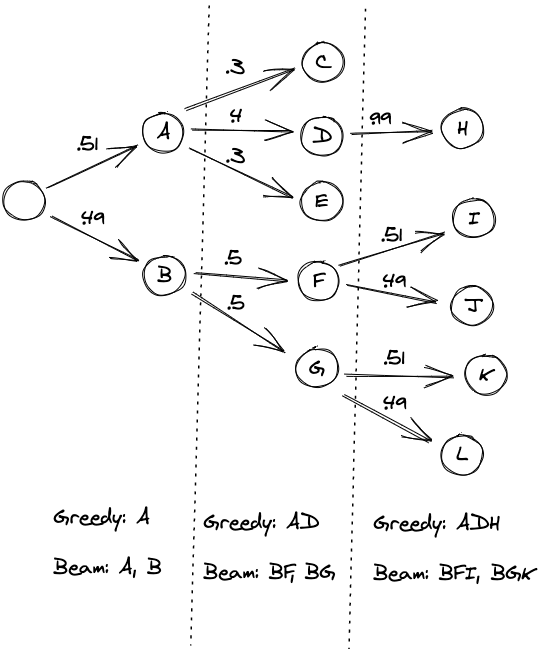
\includegraphics[scale=0.4]{beamsearch_vs_greedsearch.png}
	\caption{Принцип получения предсказания посредством жадного поиска и лучевого поиска.  \cite{vitalflux}.}
	\label{fig:beamsearch_vs_greedsearch}
\end{figure}

\subsection{Метрики качества в задаче создания подписей к изображениям}

Оценить качество сгенерированного текста представляется более сложной задачей нежели оценка качества классификации. Основная часть метрик основана на сравнении полученного текста с его неким эталоном, золотым стандартом. В задаче создания подписей к изображениям эталонным текстом при обучении выступают заранее созданные человеком описания.

Наиболее точной оценкой сгенерированного текста является экспертная оценка, позволяющая учесть все нюансы полученного описания. Оценивание производится по 5-тибальной шкале. Однако она является дорогой, медленной и трудоемкой, поскольку требует при расчете участие человека.

Для автоматической оценки работы сгенерированных текстов зачастую используются такие показатели как BLEU, WER, NIST, ROUGE, METEOR, TER и прочие. Рассмотрим подробнее первые две из них.

Метрика BLEU (Bilingual Evaluation Understudy) на данный момент является одной из самых популярных. Она позволяет учитывать не только точность перевода отдельных слов, но и цепочек слов (N-граммы). Как правило расчет происходит до 4-грамм. Алгоритм BLEU оценивает качество перевода по шкале от 0 до 100 на основании сравнения машинного перевода с золотым стандартом и поиска общих слов и фраз. Основная идея метрики состоит в том, что чем лучше сгенерированный текст, тем больше он должен быть похож на эталонный. Лучше всего такая метрика работает на уровне большого текста, а не на уровне предложений. На маленьком объёме текста метрика зачастую обнуляется из-за отсутствия совпадающих 4-грамм и работает некорректно. Существуют также доработанные варианты метрики, которые подходят для сравнения на уровне предложения.

Word Error Rate (в сокращении WER), или взвешенное расстояние Левенштейна, позволяет измерять расстояние между сгенерированным текстом и эталонным. По сути, WER измеряет минимальное количество операций (замена, удаление, добавление слова), которые необходимо сделать, чтобы из сгенерированного моделью текста получить золотой стандарт (см. формулу \ref{wer}).

\begin{equation}
	\label{wer}	
	WER = \frac{\#substitutions + \#deletions + \#insertions}{caption-output-lemgth}
\end{equation}

Данные метрики являются простыми и быстрыми оценками качества сгенерированных текстов, коррелирующих с экспертной оценкой. Однако они оперируют только короткими фрагментами, не позволяя оценить общую корректность предложения. Их сложно сравнивать между собой, поскольку оценки носят относительный характер. Также с помощью них невозможно оценить жанровую специфику текста. Еще одним их недостатком является их не дифференцируемость, не позволяющая их использовать в качестве функции потерь, то есть оптимизировать напрямую.


\subsection{Вывод}\label{subsection:conclusion}

Проведя анализ текущих подходов к решению задач многоклассовой классификации и создания подписей к изображениям, было решено остановиться на архитектуре «Encoder-Decoder», где данные части будут представлены нейронными сетями. Однако в нее было внесено одну существенное изменение – разделение блока «Encoder» и «Decoder» и обучение их по отдельности. Обучение «Encoder» происходило на задачу классификации, «Decoder» - на задачу генерации описании (см. рисунок \ref{fig:general_encoderdecoder_scheme}).

\begin{figure}[ht]
	\centering
	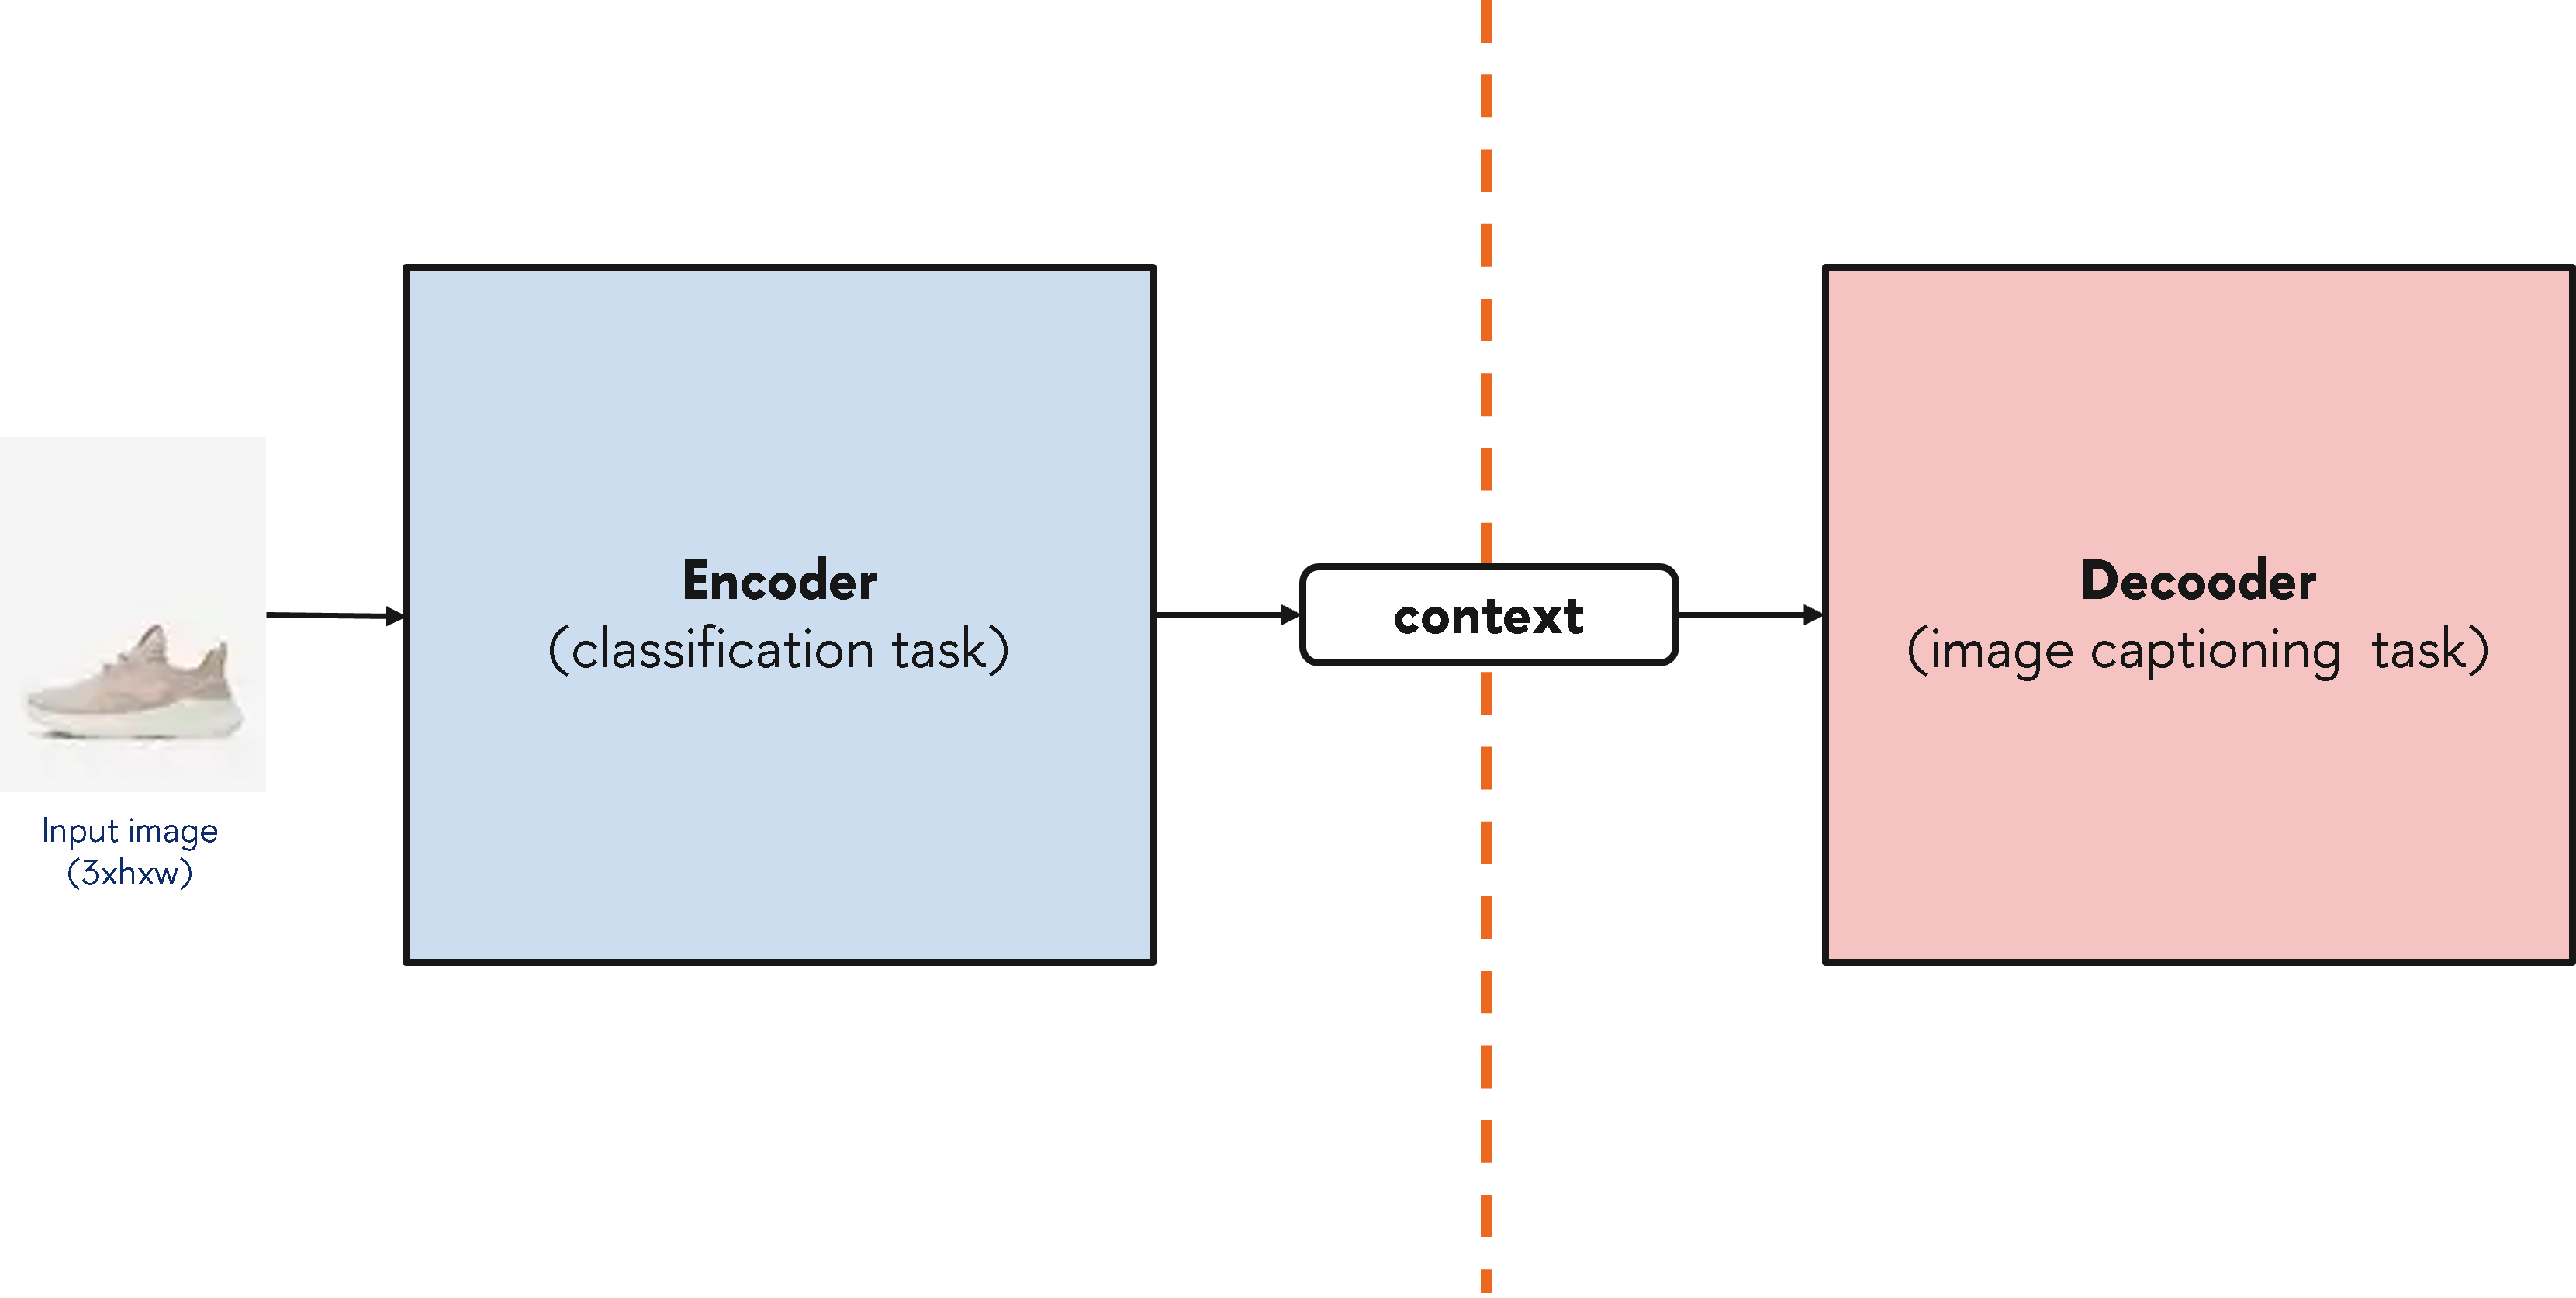
\includegraphics[scale=0.5]{general_encoderdecoder_scheme.png}
	\caption{Общая схема архитектуры модели.}
	\label{fig:general_encoderdecoder_scheme}
\end{figure}

Таким образом, следующей задачей стала проверка работоспособности данной схемы в целом. Вследствие было принято решение пойти снизу вверх, от простого к сложному, с постепенным усложнением архитектуры. Другим фактором, повлиявшим на решение начать реализацию с архитектуры CNN + RNN, а не сразу переходить на модели на основе трансформеров, стал факт неоднозначности выбора в пользу того или другого подхода. В классификационных моделях сверточные нейронные сети до сих пор остаются конкурентоспособными. Для достижения качества классификации, сравнимого со сверточными моделями, ViTs требуют значительного объема данных для обучения, значительных вычислительных ресурсов и много дополнительных действия для достижения удовлетворяющего качества классификации. В то время как сверточные нейронные сети «заводятся из коробки», и при минимальных действиях возможно получение высокого качества. В задаче генерации описаний неоспоримым доминатом по качеству создаваемых текстов являются модели трансформеров. Однако, как упоминалось в разделе \ref{subsection:image-captioning}, это очень «тяжелые» модели, требующие больших вычислительных мощностей. Рекуррентные нейронные сети, хотя уступают им по качеству генераций, являются легковесными, что может сыграть решающую роль при необходимости запуска разрабатываемого приложения на малых мощностях, и более быстрыми в выдаче предсказаний, что следует принимать во внимание при важности фактора времени, которое будет затрачено на получение предсказания.

Дальнейшим этапом работы стала реализация базовых CNN в качестве кодировщика и RNN в качестве декодировщика с их последующим усложнением, таким как разработка концептуально новых решений, позволяющих повысить качество классификации с учетом особенностей используемых данных, использование нескольких последовательных и параллельных блоков RNN, а также добавление механизма внимания, применяя разные способы его реализации. При успешном исходе для повышения качества генерации будет выполнен переход блоков энкодера и декодера на модели трансформеров.



\newpage
\section{Эксперименты}

\subsection{Общие принципы обучения}

В данном разделе будет детальное описание способов, методов и приемов реализации модели. Для лучшего понимания обратимся к ключевой идее данной работы: должна быть разработана модель, которая по присланной фотографии товара определяет к какой категории изображенный объект лучше отнести и генерирует к нему описание. Таким образом, одновременно должны решаться задача классификации и задача генерации текстового описания по изображению. Как было описано в теоретических основах (см. раздел \ref{subsection:conclusion}), поставленная задача будет решается с использованием архитектуры «Encoder-Decoder», где, из-за потребности решения одновременно двух задачи, обучение блоков «Encoder» и «Decoder» происходит по отдельности: обучение «Encoder» происходило на задачу классификации, «Decoder» - на задачу генерации описании (см. рисунок \ref{fig:general_encoderdecoder_scheme}). Другими введенными ограничениями являлось использование свёрточных нейронных сетей в качестве кодировщика и рекуррентных сетей в качестве декодировщика.

Опишем принцип построения разработанной схемы (см. рисунок \ref{fig:general_scheme}). Входными данными выступает фотография товара, которая подается в «encoder». Кодировщик состоит из backbone, инициализированный предобученными весами на ImageNet и частично замороженным (см. раздел \ref{subsection:results-classification}), и двух линейных слоев, соединенных функцией активации. Первый линейный слой отвечает за формирование эмбединга для изображения, который впоследствии будет подан в «decoder», второй – непосредственно за классификацию. После получения предсказания классификатора, сформированный эмбединг подается в качестве контекста декодировщику, который производит генерацию текста. Размер эмбединга изображения был выбран экспертным путем и равнялся 1024.

\begin{figure}[ht]
	\centering
	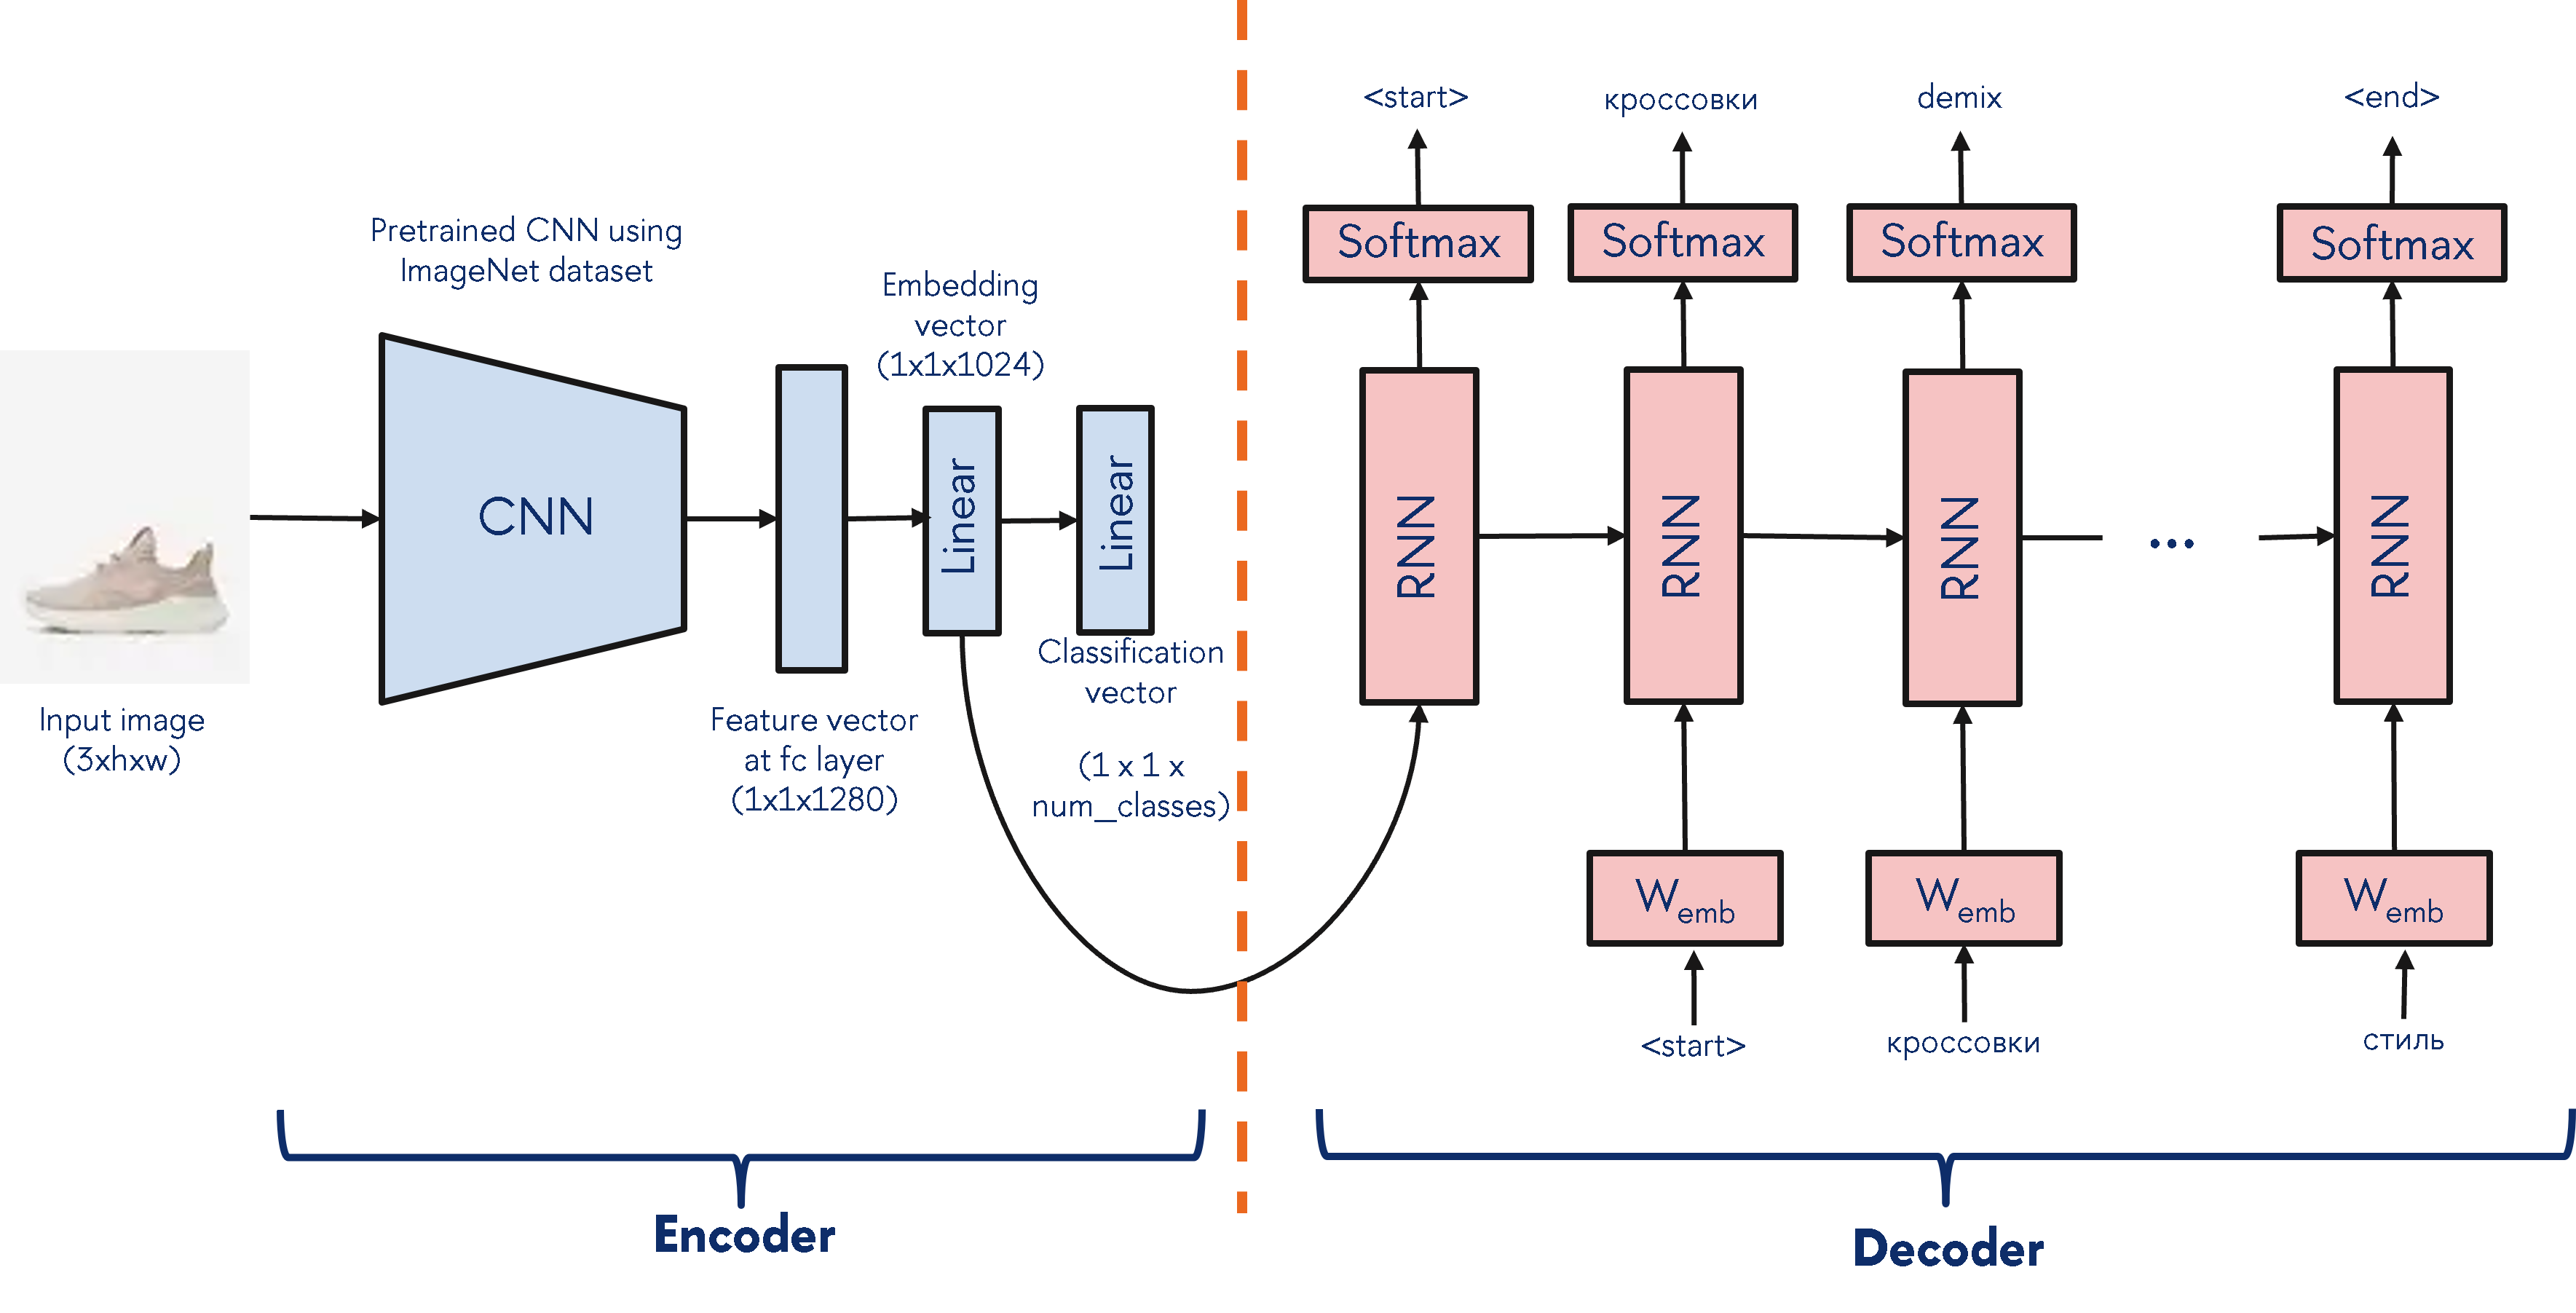
\includegraphics[scale=0.55]{general_scheme.png}
	\caption{Архитектура реализуемой модели.}
	\label{fig:general_scheme}
\end{figure}

Необходимо отметить, что поскольку эмбединги изображения формируются в кодировщике, обучающемся только на задачу классификации, их формирование может происходить не оптимально для задачи генерации текста, что может отразиться на качестве полученных описаний.

Для справедливости стоит отметить, что подобная схема\footnote{В частности, схема кодировщика.} была подобрана посредством экспериментов и исходя из требований, налагающимися на нее выдвинутыми ранее ограничениями. Во-первых, в кодировщике необходим линейный слой, отличный от классификационного, для получения эмбединга изображения. Во-вторых, для реализации в RNN второго из видов внимания, описанного на странице 42, требовались отдельные эксперименты с использованием в качестве контекста для RNN трехмерных представлений изображения, доставаемых из более ранних слоев предобученной CNN.

В экспериментах тестировались разные размеры embedding vector\footnote{Все обозначения берутся согласно схеме \ref{fig:general_scheme}.}, функции активации между слоями, варианты dropout и batch-нормализации, добавление большего числа линейных слоев в голове. Была опробована схема, изображенная на рисунке \ref{fig:general_scheme2} с параллельным обучением двух эмбедингов и последующей их конкатенации, также имели место варианты с использованием в качестве контекста для RNN эмбединга из «feature vector at fc layer» или из более ранних слоев. 
\begin{figure}[ht]
	\centering
	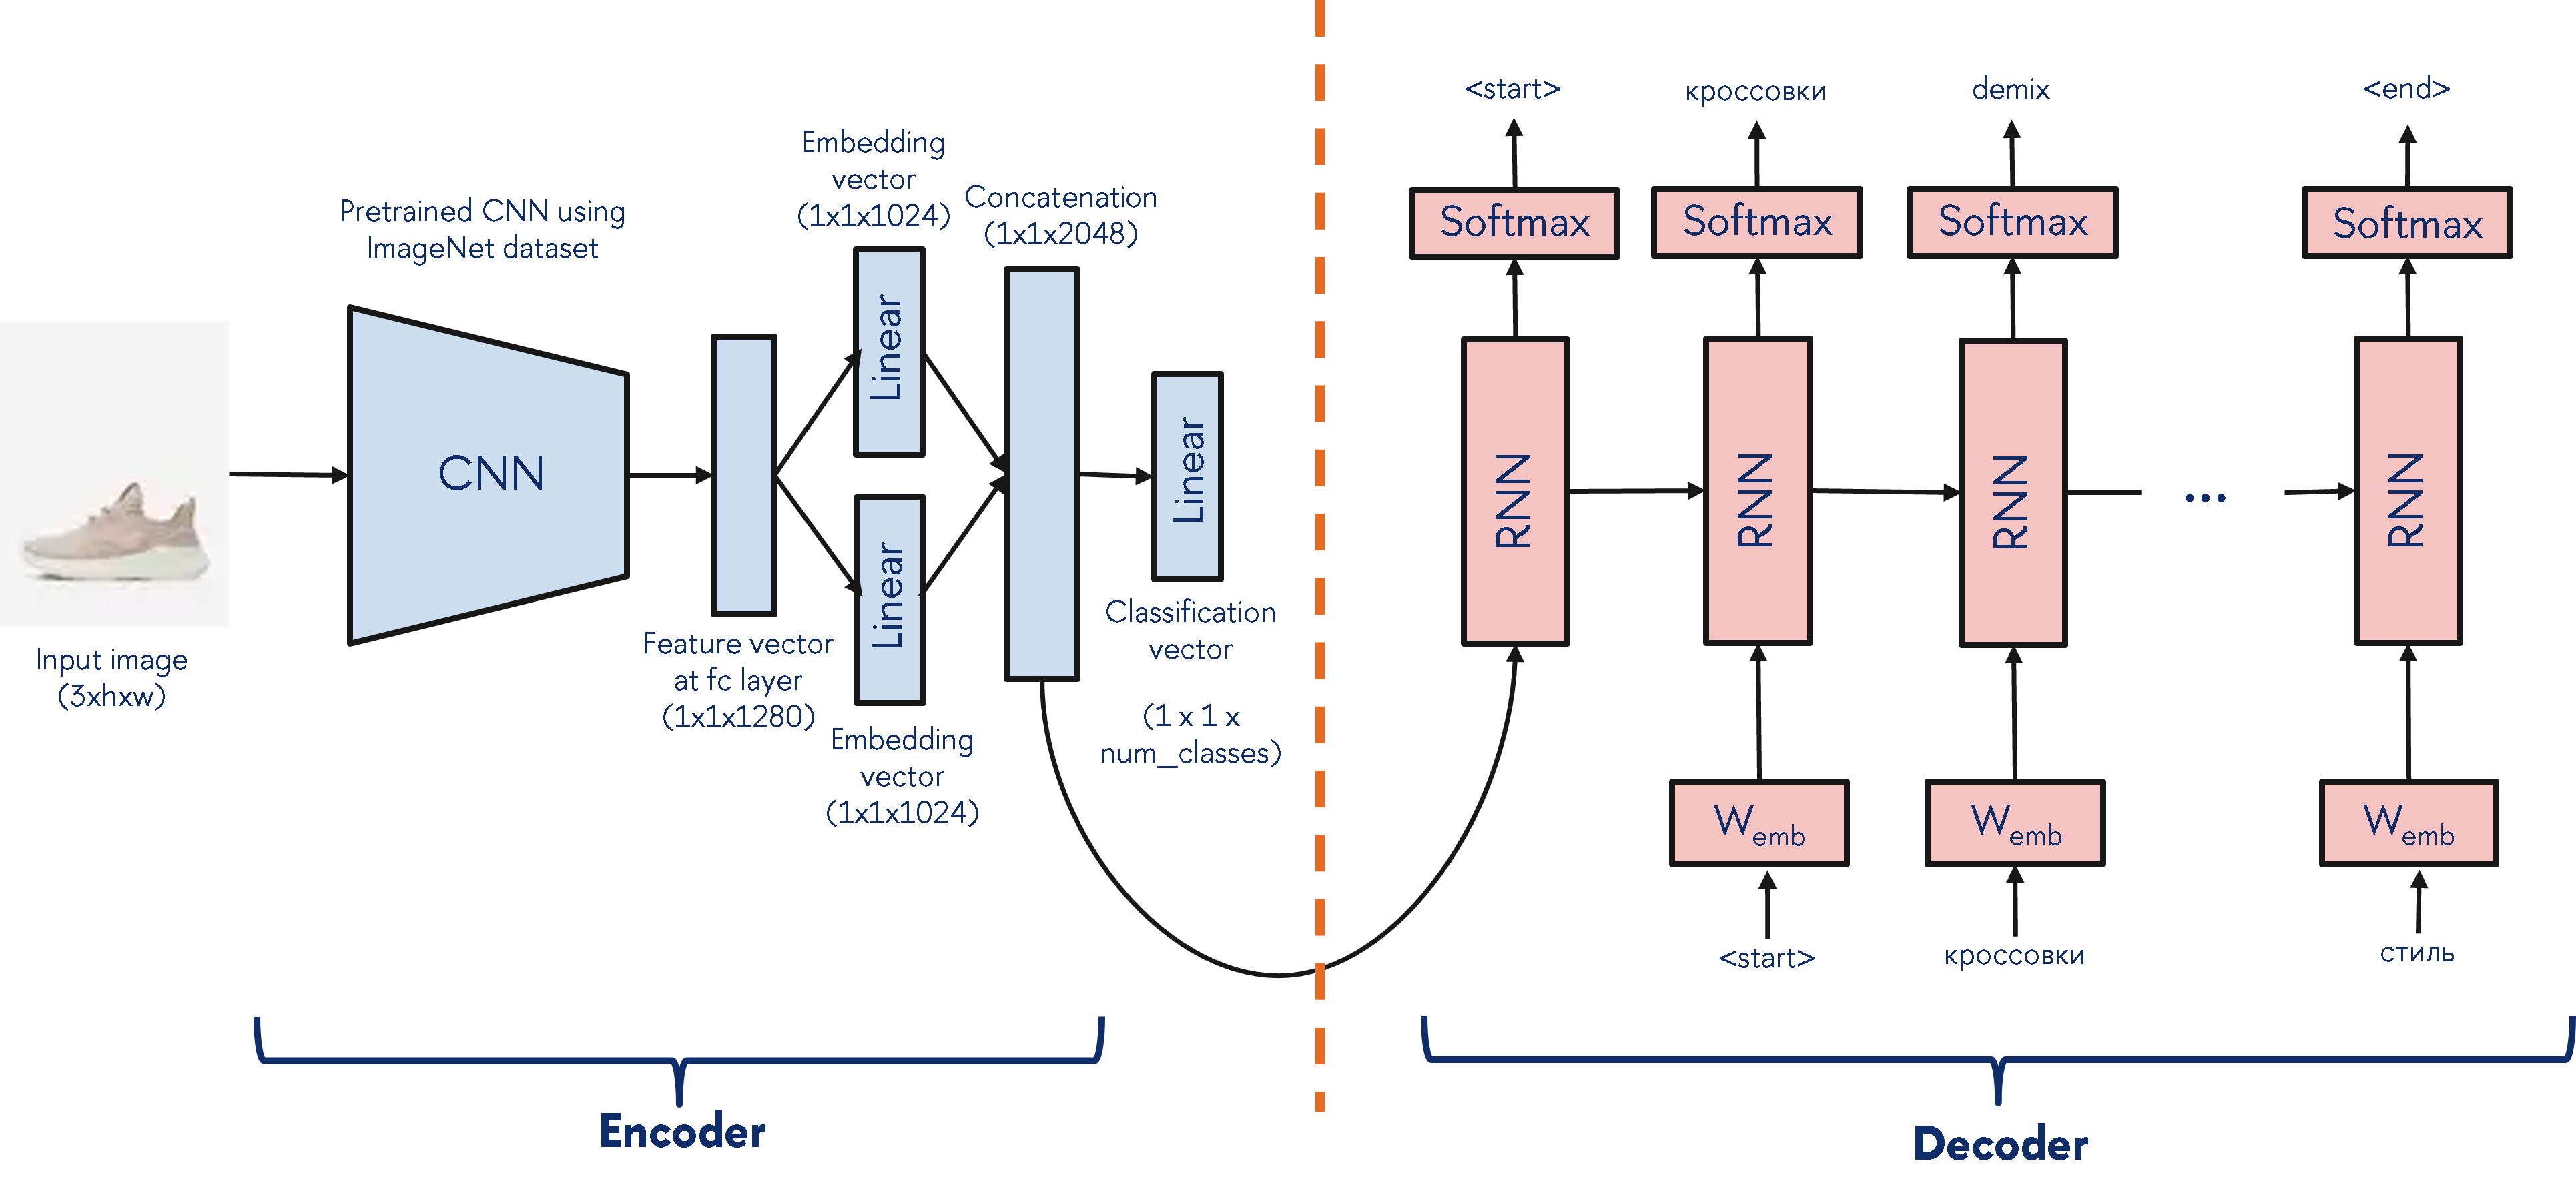
\includegraphics[scale=0.55]{classification/general_schemev2.png}
	\caption{Альтернативная архитектура модели.}
	\label{fig:general_scheme2}
\end{figure}
Однако, все вышеперечисленные эксперименты проверялись посредством качества классификации и однозначно предугадать влияние того или иного варианта на качества генерации описания к изображениям нельзя. Наиболее важным и самым сложным в тестировании качества выступал размер embedding vector\footnote{Данное утверждение становится понятным, принимая во внимание финальный выбор архитектуры кодировщика, более детально описанный в разделе \ref{subsection:results-classification}}.


\subsection{Решение задачи классификации}\label{subsection:results-classification}

Первым шагом в решении задачи классификации было обучение единой модели для всех конечных категорий\footnote{После очистки данных осталось 1385 конечных категорий.} (см. рисунок \ref{fig:classification_onemodel}). 

\begin{figure}[ht]
	\centering
	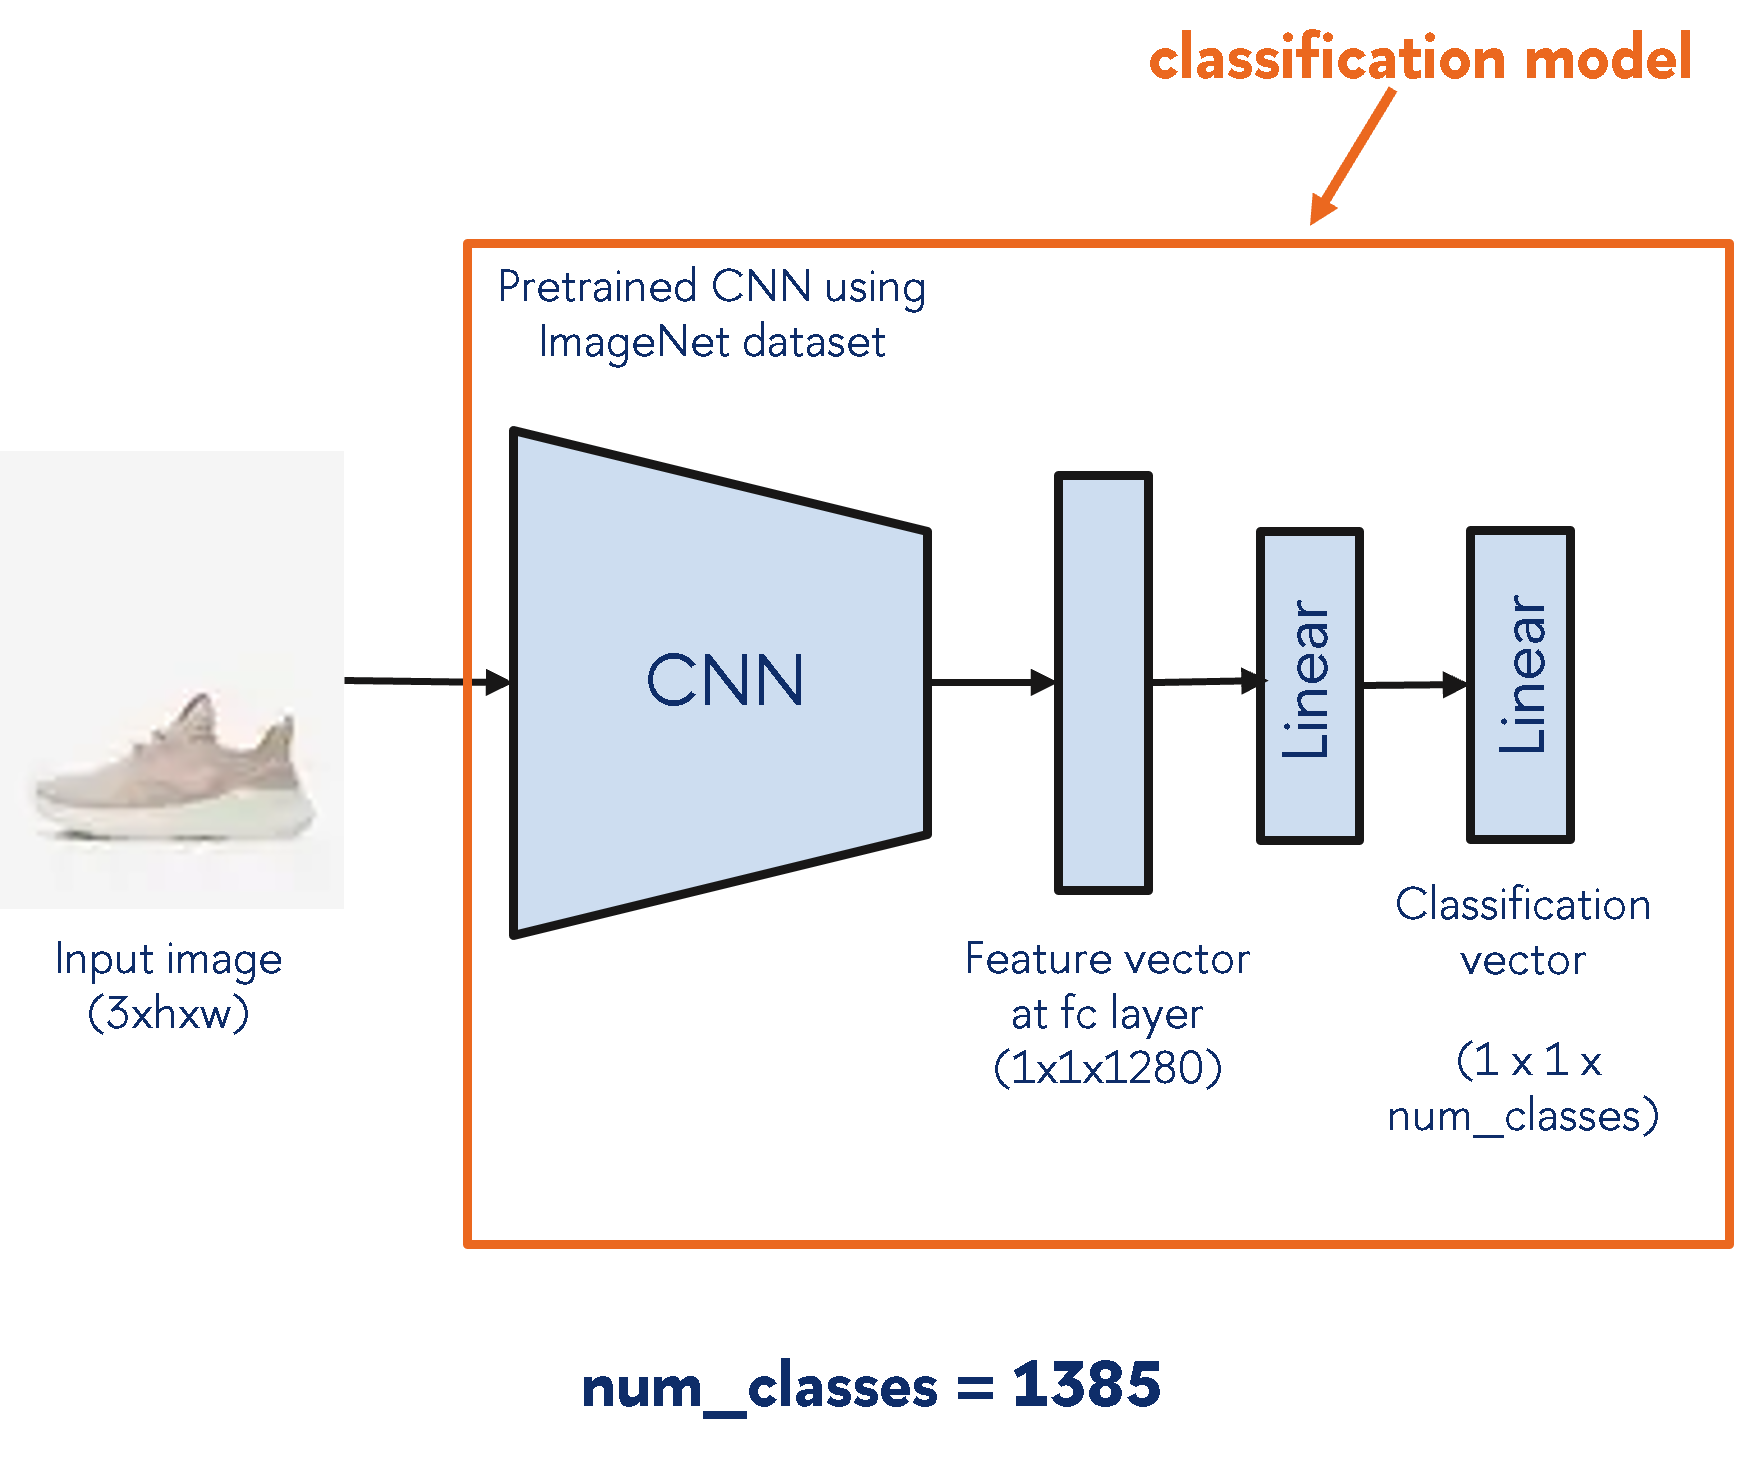
\includegraphics[scale=0.7]{classification/classification_onemodel.png}
	\caption{Архитектура единой классификационной модели для всех классов.}
	\label{fig:classification_onemodel}
\end{figure}

Данный вариант имел ряд серьезных недостатков, из-за которых впоследствии было решено от него отказаться:
\begin{itemize}
	\item Во-первых, для качественного обучения классификационной модели с большим количеством категорий требуется довольно много примеров, чтобы модель смогла выявить особенности каждого класса. Это объясняется тем, вероятностная масса размывается на большое количество классов, что делает модель менее устойчивой. В рамках данного проекта в каждой категории имелось в распоряжении около 20 объектов, что было явно недостаточно. Более того, данные являются достаточно шумными, усугубляя общую картину. Следствием этого выступило низкое качество классификатора, не удовлетворяющее минимальные требования (см. таблицу \ref{table:metrics_all}).
	
	\begin{table}[ht]
		\caption{Метрики качества модели, обученной на все конечные категории.}
		\label{table:metrics_all}
		\footnotesize
		\centering
		\begin{tabular}{l|l}
			\toprule
			\multicolumn{1}{c|}{metric} & \multicolumn{1}{c}{value}\\
			\midrule
			accuracy           & 0.4708\\
			accuracy@top2      & 0.6154\\
			precision macro    & 0.4768\\
			recall macro       & 0.4644\\
			f1 macro           & 0.4466\\
			precision micro    & 0.4708\\
			recall micro       & 0.4708\\
			f1 micro           & 0.4708\\
			precision weighted & 0.4824\\
			recall weighted    & 0.4708\\
			f1 weighted        & 0.4526\\
			\bottomrule
		\end{tabular}
	\end{table}
	
	\item Во-вторых, из-за больших размеров модели время обучения даже на текущем датасете было очень велико, что затрудняло подбор оптимальный гиперпараметров. Следствием из этого будет выступать такое же неудовлетворительное по длительности время последующего дообучения/переобучения модели на новых данных.
	\item В-третьих, поскольку конечная матрица имеет внушительные размеры, время получения предсказаний также оставляло желать лучшего. (ЗАМЕРИТЬ ВРЕМЯ ИНФЕРЕНСА)
\end{itemize}

Решением указанных недостатков стало получение предсказания посредством дерева моделей. Будем называть архитектуру модели, изображенной на рисунке 1, classification model. Тогда принцип архитектуры дерева моделей будет выглядеть следующим образом: см. рисунок \ref{fig:classification_treemodel}. Заранее обучается n классификаторов по количеству материнских категорий, каждый из которых обучен на классы, соответствующие данным материнским категориям. Для получения предсказания входное изображение сперва подается в классификационную модель, обученную на классы первой вложенности. Далее в зависимости от предсказанной категории, полученной из данной модели, и при условии, что категория является материнской, картинка передается на вход следующему классификатору, обученному на подкатегории выбранной материнской категории. Данная процедура продолжается до тех пор, пока предсказание какого-либо из классификаторов не окажется конечной категорией.

\begin{figure}[ht]
	\centering
	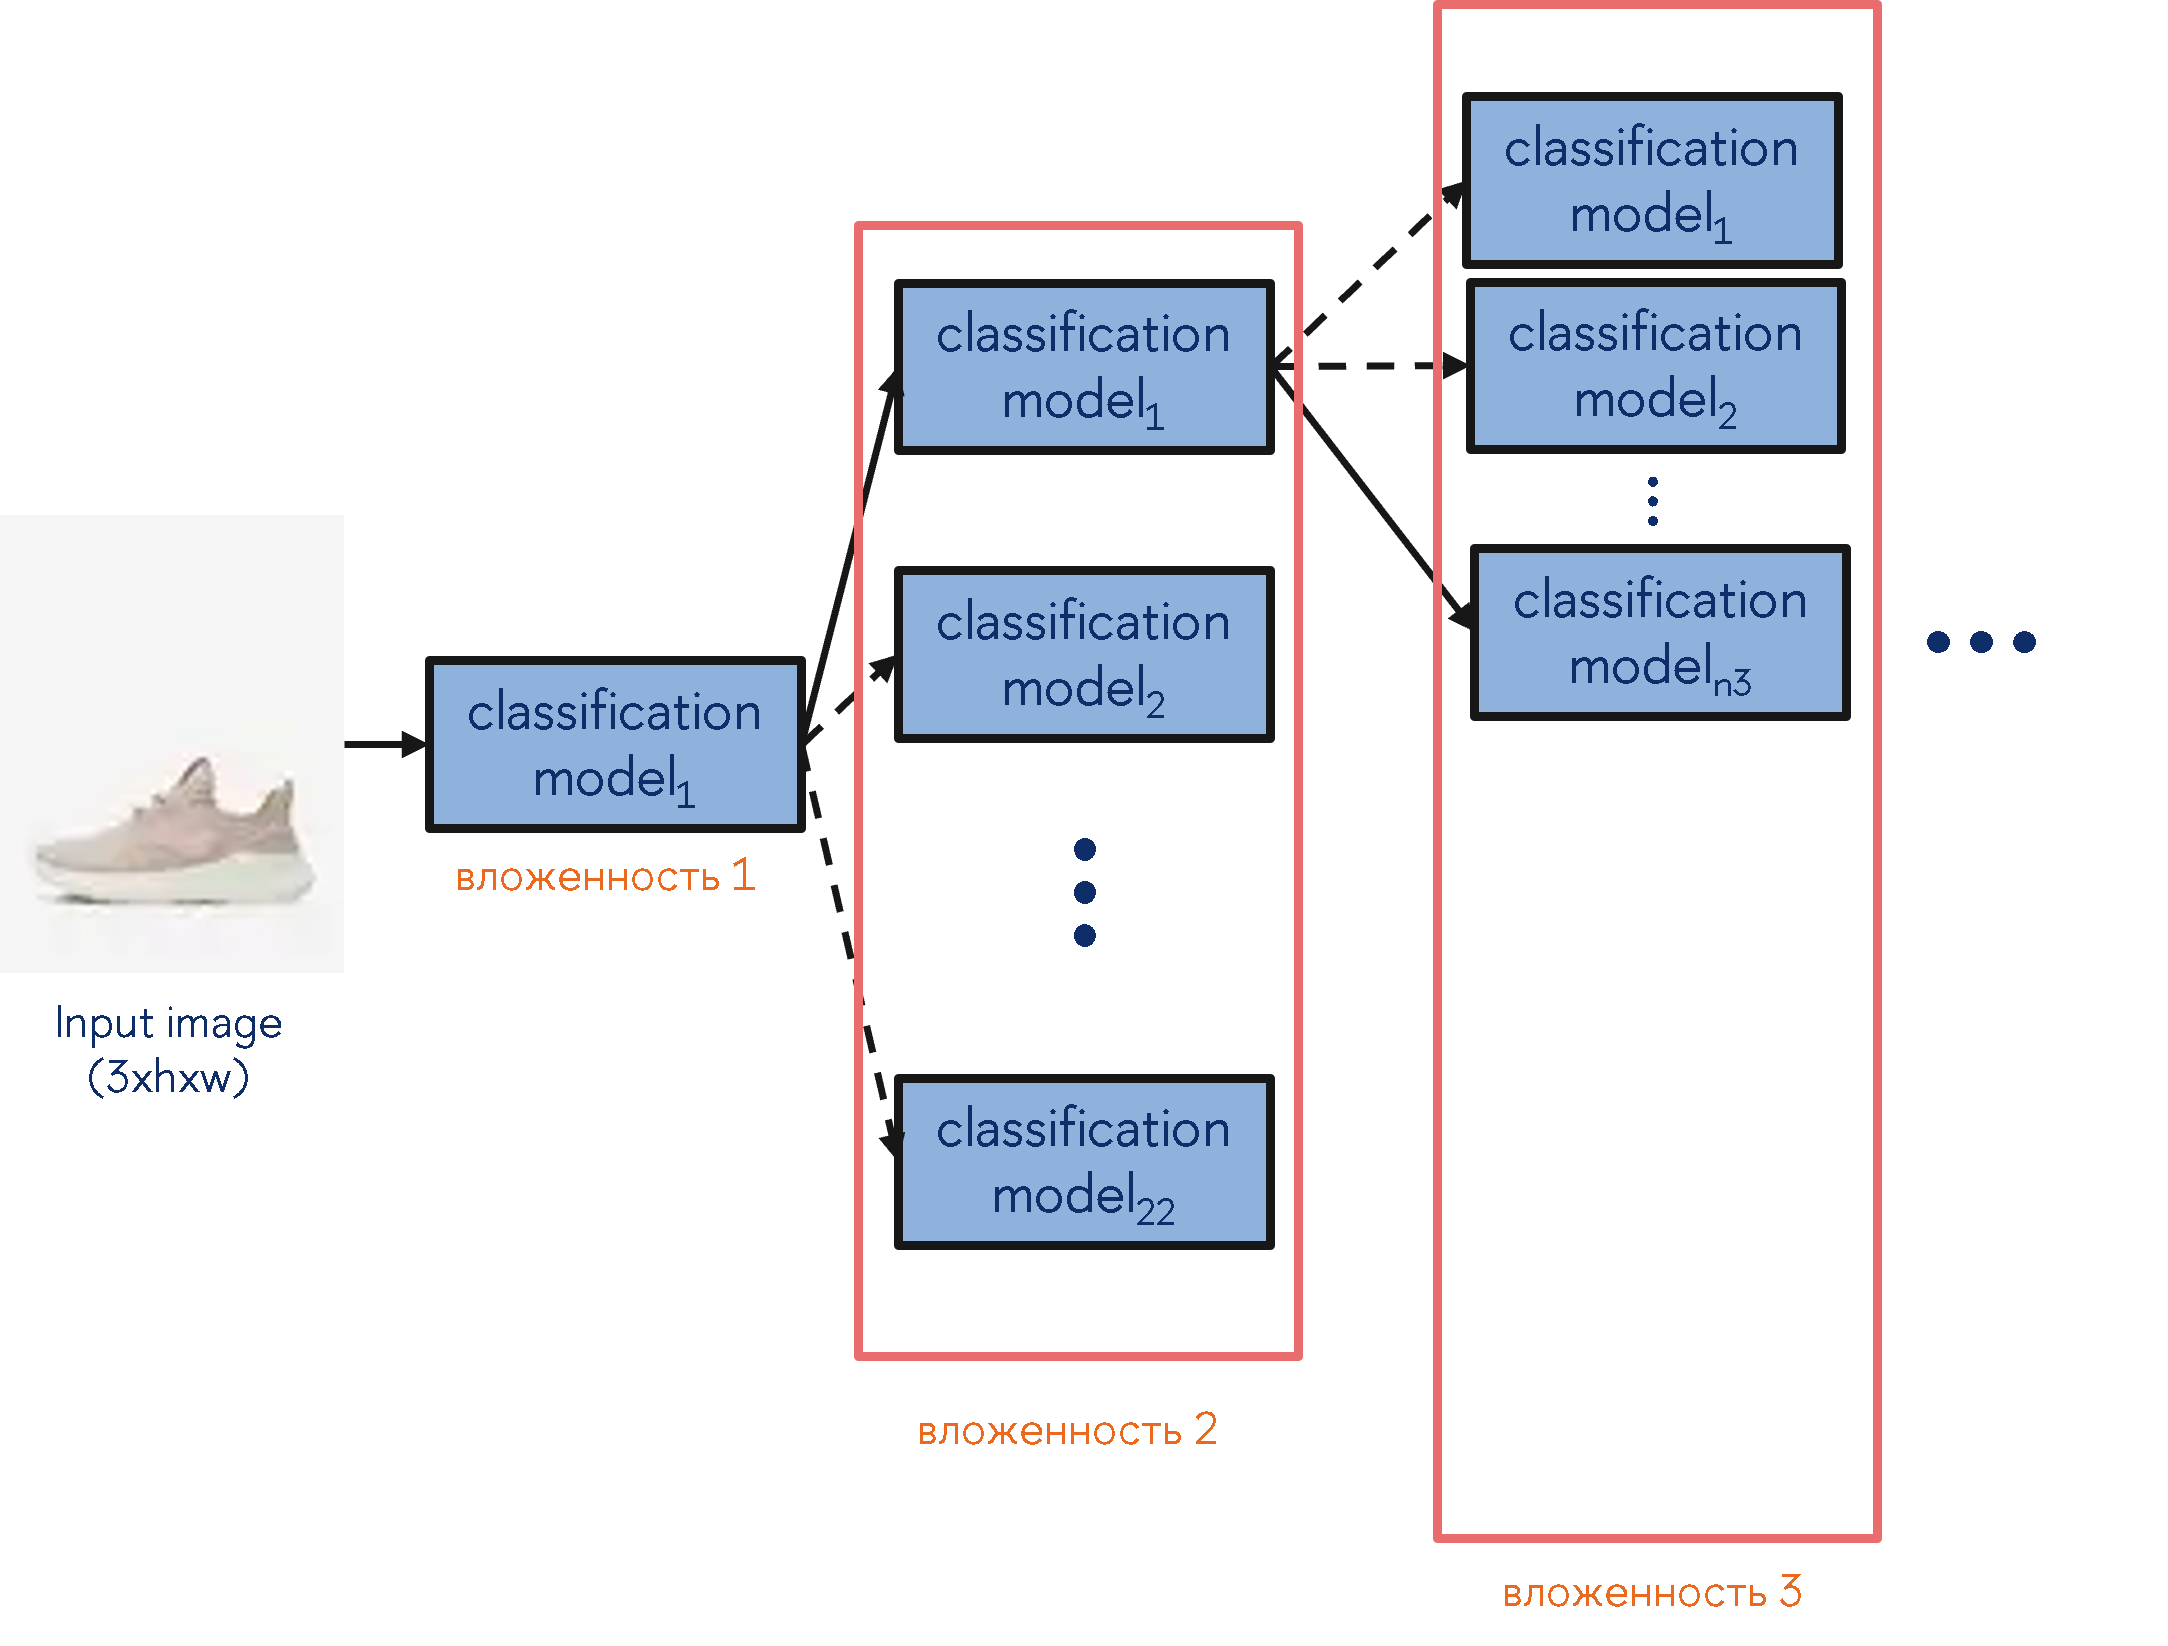
\includegraphics[scale=0.7]{classification/classification_treemodel.png}
	\caption{Архитектура дерева классификационных моделей.}
	\label{fig:classification_treemodel}
\end{figure}

Поясним подробнее процедуру формирование классов для моделей на примере категории «Канцтовары». Основная идея заключается в объединении всех нижележащих подкатегорий в материнскую категорию. Таблицы \ref{table:gettarget2} и \ref{table:gettarget3} показывают, как конечные категории раздела «Канцтовары» преобразовывались в классы для моделей второй и третьей вложенности соответственно. Структура сохранения данных при сборе была продумала таким образом, чтобы формирование классов для дерева моделей происходило максимально удобным образом. Ключевая идея состояла в составлении названия папок, содержащих данные по одной конечной категории, таким образом, чтобы при необходимости можно было с легкость проследить путь, ведущий от категорий первой вложенности к конкретной конечной категории.

\begin{table}[ht]
	\caption{Преобразование классов для модели "Канцтовары" (вторая вложенность), фрагмент.}
	\label{table:gettarget2}
	\footnotesize
	\centering
	\begin{tabular}{ll}
		\toprule
		\multicolumn{1}{c}{название папки} & \multicolumn{1}{c}{класс}\\
		\midrule
		Канцтовары\_Анатомические\&модели & Анатомические\&модели\\  Канцтовары\_Бумажная\&продукция\_Блокноты & Бумажная\&продукция\\
		Канцтовары\_Бумажная\&продукция\_Гостевые\&книги & Бумажная\&продукция\\
		Канцтовары\_Бумажная\&продукция\_Дневники & Бумажная\&продукция\\
		Канцтовары\_Бумажная\&продукция\_Закладки & Бумажная\&продукция\\
		Канцтовары\_Бумажная\&продукция\_Наклейки & Бумажная\&продукция\\
		Канцтовары\_Карты\&и\&глобусы & Карты\&и\&глобусы\\
		Канцтовары\_Письменные\&принадлежности & Письменные\&принадлежности\\
		Канцтовары\_Рисование\&и\&лепка & Рисование\&и\&лепка\\
		Канцтовары\_Чертежные\&принадлежности & Чертежные\&принадлежности\\
		... & ...\\
		\bottomrule
	\end{tabular}
\end{table}

\begin{table}[ht]
	\caption{Преобразование классов для модели \\ "Канцтовары\_Бумажная\&продукция" (третья вложенность), фрагмент.}
	\label{table:gettarget3}
	\footnotesize
	\centering
	\begin{tabular}{ll}
		\toprule
		\multicolumn{1}{c}{название папки} & \multicolumn{1}{c}{класс}\\
		\midrule
		Канцтовары\_Бумажная\&продукция\_Блокноты & Блокноты\\
		Канцтовары\_Бумажная\&продукция\_Гостевые\&книги & Гостевые\&книги\\
		Канцтовары\_Бумажная\&продукция\_Дневники & Дневники\\
		Канцтовары\_Бумажная\&продукция\_Закладки & Закладки\\
		Канцтовары\_Бумажная\&продукция\_Наклейки & Наклейки\\
		... & ...\\
		\bottomrule
	\end{tabular}
\end{table}

Описанное решения на первый взгляд может показаться очень громоздким и неоправданно усложненным. Получение предсказание через дерево моделей позволяет поднять поставленной качество классификационной задачи в целом. Это объяснено тем, что задача на меньшее количество классов решается априори лучше. Другим достоинством предложенного подхода является уменьшение времени получения предсказаний, поскольку прогон через несколько небольших моделей происходит быстрее, чем через одну большую.

С переходом на подобную модель классификации возникает вопрос ее адаптации к задаче image captioning. Появление нескольких классификаторов поднимает вопрос получения эмбединга изображения для декодировщика, что может решаться несколькими способами. Например, можно брать эмбединг изображения с самой глубокой модели, то есть той модели, которая предсказала конечную категорию. Другим вариант является конкатенация эмбедингов, полученных из моделей, принявших участие при получении предсказания. Также можно вместо конкатенации применить взвешивание данных эмбедингов с определенными весами. В работе был использован первый вариант, несмотря на очевидный его недостаток – при получении эмбединга изображения из глубоких классификаторов появляется риск забывания моделью важных общих характеристик объекта (например, чем дамская сумочка отличается от рюкзака) и фокус на мелких деталях (например, как дамскую сумку от фирмы Gucci отличить от сумки фирмы Chanel). Другие упомянутые варианты отпали по причине разного количества моделей, участвующих при получении того или иного предсказания. В этом случае необходимо было разрабатывать дополнительные специфичные приемы, позволяющие получить одинаковый размер финального эмбединга изображения.

После принятия решения об использовании для декодировщика эмбедингов, полученных из самой глубокой модели возникает следующая проблема, требующая решения: как избежать ситуации, когда полученные из разных моделей эмбединги изображения и, соответственно, означающие разные классы, будут численно одинаковыми. Решение данной проблемы стала заморозка большинства слоев backbone и получение эмбедингов из более-менее одного смыслового пространства, что уменьшает вероятность возникновения подобных ситуаций. При проведении экспериментов наиболее оптимальным уровнем размораживания backbone стала разморозка двух последних слоев\footnote{В частности, последний блок MBConv и блок активации Conv2dNormActivation.}. Это позволяло поднять качество классификаций на 5-10 процентных пунктов. С другой стороны, подобная заморозка уменьшает время обучения и последующих дообучений модели, потому что происходит обучение только линейной головы классификатора. Кроме того, уменьшается размер необходимого дискового пространства, необходимого для хранения весов классификаторов, поскольку необходимым становится только хранение весов для размороженных слоев и линейных голов моделей. Также стоит отметить значительное облегчение процесса переобучения и дообучения классификаторов, так как архитектура дерева моделей не требует единовременного переобучения всех моделей и классов. Другими словами, переобучение может затрагивать только необходимые модели, никак не касаясь других классификаторов. Таким образом, поддержания в актуальном состоянии большого количества классификационных моделей не будет являться проблематичным. Еще одним достоинством применения замораживания основной части backbone является уменьшение времени, необходимое на получение предсказания, по сравнению с полностью размороженной моделью. Аргументировано это тем, что при передаче изображения между моделями в дереве будет происходить только переинициализация весов головы моделей.

Следующей досадной неприятностью при переходе на архитектуру получения предсказания посредством дерева моделей может стать количество классификаторов, необходимых к обучению. Данная цифра напрямую зависит от структуры каталога и детализированности категорий выбранного маркетплейса. Как было упомянуто в разделе \ref{subsection:datastep1}, максимально было до пяти уровней вложенности. Другими словами, максимальная глубина дерева моделей – 5. Однако кроме глубины дерева важную роль играет его ширина. В таблице \ref{table:amount-models} представлено количестве моделей, которое должно быть обучено в зависимости от выбранной глубины вложенности.

\begin{table}[ht]
	\caption{Количество моделей, необходимые к обучению в зависимости от уровня вложенности.}
	\label{table:amount-models}
	\footnotesize
	\centering
	\begin{tabular}{cc}
		\toprule
		\multicolumn{1}{c}{кол-во моделей} & \multicolumn{1}{c}{уровень вложенности}\\
		\midrule
		171 & вложенность 5\\
		165 & вложенность 4\\
		153 & вложенность 3\\
		22  & вложенность 2\\
		1   & вложенность 1\\
		\bottomrule
	\end{tabular}
\end{table}

Можно заметить, что значительная детализация категорий происходит на третьем уровне вложенности. Принимая во внимание цели данной работы, которые заключаются в том числе в проверке работоспособности предложенной архитектуры в целом, было решено остановиться на втором уровне вложенности. Таким образом, происходило обучение 22 классификационных модели. В таблице \ref{table:modelstatistic1} представлена статистика по размерам датасетов, на которых были обучены модели классификации. Согласно пятидесятому квантилю, ровно в половине моделей количество данных не превышало 1000. Однако (см. также \ref{fig:amount_of_categoty}) нельзя не обратить внимания на большой размах в размере категорий: какие-то модели были обучены на 5000 примерах, какие-то только на 300.

\begin{table}[ht]
	\caption{Описательная статистика по размерам датасетов для моделей в дереве классификаций (слева - по второй вложенности, справа - по всем моделям).} 
	\label{table:modelstatistic1}
	\footnotesize
	\centering
	\begin{tabular}{l|r}
		\toprule
		{} & \multicolumn{1}{c}{dataset size}\\
		\midrule
		count &	20\\
		mean  & 1283.75\\
		std   & 1226.88\\
		min   &	264.00\\
		25\%  &	484.00\\
		50\%  &	954.50\\
		75\%  &	1660.25\\
		max   &	5720.00\\
		\bottomrule
	\end{tabular}
	\hspace{2cm}
	\begin{tabular}{l|r}
		\toprule
		{} & \multicolumn{1}{c}{dataset size}\\
		\midrule
		count &	20\\
		mean  & 1283.75\\
		std   & 1226.88\\
		min   &	264.00\\
		25\%  &	484.00\\
		50\%  &	954.50\\
		75\%  &	1660.25\\
		max   &	5720.00\\
		\bottomrule
	\end{tabular}
\end{table}

В обоих подходах при проведении экспериментов в качестве сверточных нейронных сетей брались MobileNetV2 из-за своей компактности и быстроте, а также семейство моделей EfficientNetV2 из-за их высокого качества практически на всех стандартных наборах данных. Финальной моделью была выбрана EfficientNetV2-S, сочетающая в себе оптимальный баланс качества классификаций и затрат на время обучения.

Другими используемыми приемами при обучении классификаторов было добавление аугментаций. При обучении всех моделей использовались аугментации, смешивающие разные изображения (в частности MixUp и CutMix\cite{cutmix}). Использование настолько сильных аугментаций являлось необходимым в связи сильным переобучение моделей под обучающий набор данных, который был вызван отчасти их небольшим размером. Другие виды аугментаций подбирались при оптимизации модели и составляли индивидуальный набор для каждого классификатора. В качестве оптимизатора лучше всего себя показал AdamW\footnote{\url{https://pytorch.org/docs/stable/generated/torch.optim.AdamW.html}} (адаптивный градиентный шаг с использованием momentum и weight decay). Также часть классификаторов потребовала использование шедуллера (англ. scheduler) для изменения градиентного шага (англ. learning rate). В основном использоваться CosineAnnealingLR\footnote{\url{https://pytorch.org/docs/stable/generated/torch.optim.lr_scheduler.CosineAnnealingLR.html}}. В качестве функции потерь использовался CrossEntropyLoss\footnote{\url{https://pytorch.org/docs/stable/generated/torch.nn.CrossEntropyLoss.html}}c применением техники label smoothing.

\subsubsection{Результаты классификации}

Как было описано в разделе \ref{classification_metrics}, для каждой модели рассчитывались такие метрики как accuracy, precision, recall, f1 мера с использованием макроусреднения. Также строились матрица ошибок и classification\_report\footnote{\url{https://scikit-learn.org/stable/modules/generated/sklearn.metrics.classification\_report.html}}. Из интегральных метрик производилось построение ROC и PR кривых с расчетом AUC и Average Precision как для каждого класса в отдельности, так и с использование микро- и макроусреднения.

Схема расчета метрик была усложнена тем фактом, что понимания качества одной классификационной модели недостаточно для понимания всей классификации в целом. Для этой цели был написан ряд функций, позволяющий рассчитать данные показатели, объединенные по всем моделям, с использованием идей микро- и макроусреднения, а также их комбинации микро-макроусреднения. 

Вариант с применением принципов макроусреднения (более точнее можно охарактеризовать как макро-макро усреднение) состоял из расчета необходимых показателей (для PR-curve рассчитывались precision и recall, для ROC-curve – FPR и TPR) для каждой из 22 моделей по схеме, описанной в разделе \ref{classification_metrics}, для всех необходимых порогов отсечения. Затем полученные значения для каждого порога усреднялись с одинаковыми весами. В случае микроусреднения (более точное название микро-микро усреднение) для каждой модели для всех необходимых порогов рассчитывались элементы матрицы ошибок по алгоритму, описанному в разделе \ref{classification_metrics}. Далее по каждому порогу происходило их усреднение, и на основании полученных общих характеристик TP, FP, TN, FN производились расчеты precision и recall в случае PR-curve и FPR и TPR в случае ROC-curve. Вариант расчета микро-макро усреднения производился по принципу: для каждой модели считаются метрики посредством микроусреднения, объединение метрик по всем моделям происходит через макроусреднение. Для каждой модели в отдельности по принципу микроусреднения (см. раздел \ref{classification_metrics}) для всех требуемых порогов рассчитывались значения precision, recall для PR-curve и FPR, TPR для ROC-curve, которые впоследствии усреднялись по вероятностным порогам с одинаковыми весами. По аналогичным схемам производился расчет Average Precision и AUC. 

На рисунке \ref{fig:prcurve_general} представлены общие для всей модели классификации PR-кривые\footnote{PR-кривые для всех классификаторов можно найти в приложении \ref{appendix:pr_curves}.}, полученные посредством вышеописанных методов. Рисунок \ref{fig:roccurve_general} содержит ROC-кривые\footnote{ROC-кривые для всех классификаторов можно найти в приложении \ref{appendix:roc_curves}.}.

\begin{figure}[ht]
	\centering
	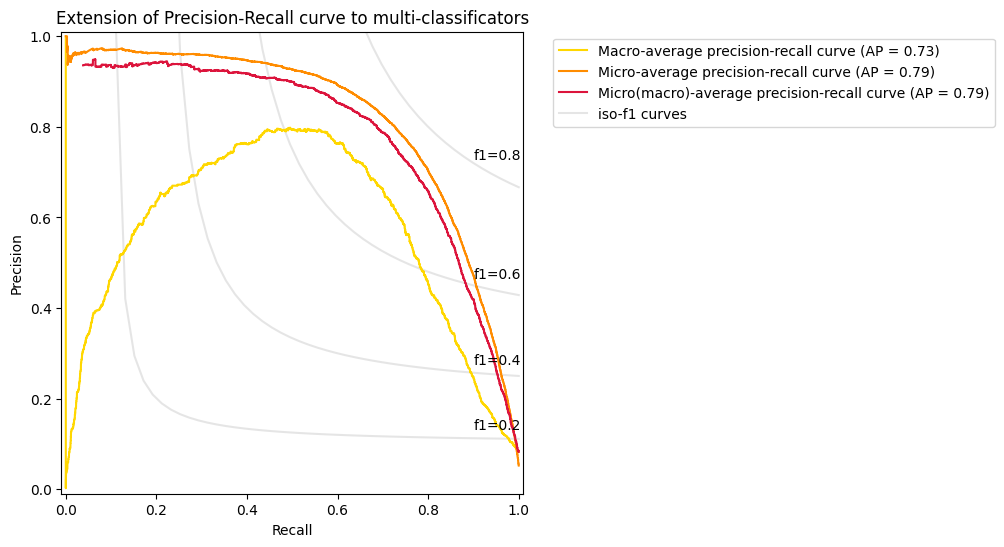
\includegraphics[scale=0.7]{pr_curves/prcurve_general.png}
	\caption{PR-curves, объединенная по всем классификационным моделям .}
	\label{fig:prcurve_general}
\end{figure}

На желтой PR-кривой, рассчитанной по принципам макроусреднения, можно заметить резкое падение значения precision в самом начале, что соответствует наиболее высоким порогам отсечения. Точно такое же проседание качества можно отметить и на двух других кривых (резкое падение оранжевой и красной кривых в левом верхнем углу), однако менее выраженное. Попробуем объяснить данное явление.

Для этого необходимо понимание значений верхних квантилей порогов отсечения, принявших участие в построении PR-кривых (см. таблицу \ref{table:quantile_prcurve_general}, а также распределение плотности точек на PR кривых. Легко заметить, что в 97\% случаях вероятности предсказаний, полученные из модели, не превышают 0.48. Что в свою очередь уже можно считать довольно неуверенными классификациями. Например, модель может предсказать, что объект с вероятностью 45\% относится к классу 1 и с вероятностью 44\% относится к классу 2. Поскольку разница в уверенностях невелика, отсюда резкое снижение true positive объектов и рост false positive объектов и вытекающее из этого понижение метрики precision. Касательно распределения плотности точек на разных частях графика, при помощи анализа было выявлено, что значение показателя recall, равное 0.5, соотносится с 37\% порогом отсечения, а recall, равный 0.2 соответствует 65\% порогу. Таким образом, правая часть графика содержит в себе несоразмерно больше точек по сравнению с левой.

\begin{table}[ht]
	\caption{Верхние квантили вероятностных порогов, участвовавших в построении PR-кривых, объединенным по всем классификационным моделям.}
	\label{table:quantile_prcurve_general}
	\footnotesize
	\centering
	\begin{tabular}{cc}
		\toprule
		\multicolumn{1}{c}{quantile} & \multicolumn{1}{c}{threshold}\\
		\midrule
		0.90 & 0.089\\
		0.91 & 0.102\\
		0.92 & 0.119\\
		0.93 & 0.145\\
		0.94 & 0.183\\
		0.95 & 0.244\\
		0.96 & 0.342\\
		0.97 & 0.484\\
		0.98 & 0.634\\
		0.99 & 0.760\\
		1.00 & 0.980\\
		\bottomrule
	\end{tabular}
\end{table}


Из всего вышеперечисленного можно сделать предположение, что в большинстве классификаторов присутствуют классы, которые моделям трудно отличать от других и в которых они не очень уверены (уверенность в 40-70\% нельзя назвать сильной). Это приводит к тому, что при определенном уменьшении порога резко возникает много false positive объектов, что приводит к падению precision. Данный вывод подтверждается еще и тем фактом, что падение значения precision при макроусреднении сильное, а последующее восстановление более долгое (левая ветвь желтой параболы) нежели при микроусреднении, поскольку вклад каждого класса в значение показателей при макроусреднении равный. В промежуточном варианте последовательного применения micro-macro усреднения (красная линия), ожидаемо, получен средний результат между желтой и оранжевой линией. 

Наиболее точные классификации происходят при порогах 30-45\%, соответствующим вершине параболы. В этом случае доверять классификатору можно на 80\% (значение precision), однако при этом он находит только 45-60\% объектов из выборки (значение recall). Обратим внимание, что данные выводы справедливы при анализе качества классификации в целом по всем моделям и могут немного отличаться в каждом индивидуальном случае.

Также стоит отметить, что ни одно из усреднений не постигает 80\% F1 показателя. Однако всех кривые пересекают 60-70\% iso-F1 линии. Следовательно, при принятии решения о выборе порога отсечения на финальное предсказания необходимо найти компромиссное решение, при котором будет приемлемо высокое доверие к классификатору и при этом он будет способен находить довольно много объектов положительного класса. 

\begin{figure}[ht]
	\centering
	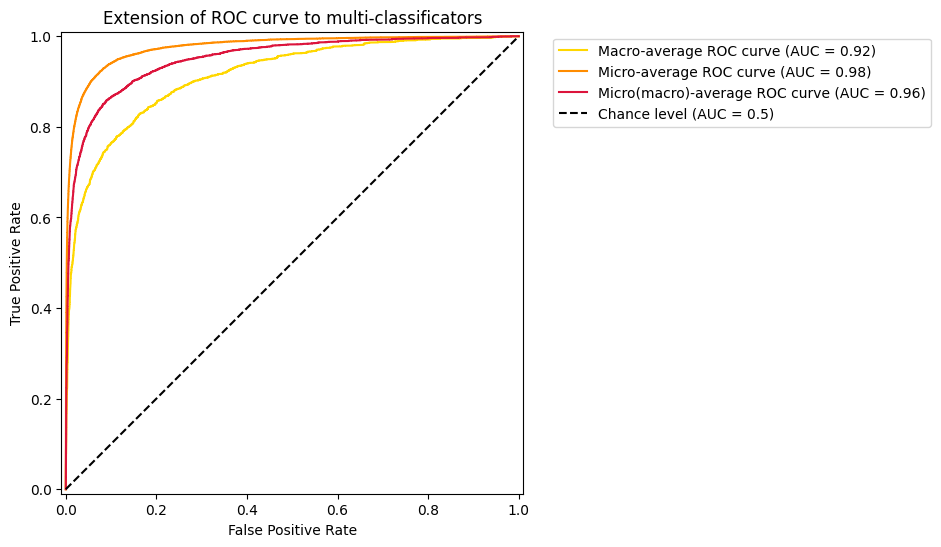
\includegraphics[scale=0.7]{roc_curves/roccurve_general.png}
	\caption{ROC-curves, объединенная по всем классификационным моделям .}
	\label{fig:roccurve_general}
\end{figure}

Как было сказано в разделе \ref{classification_metrics}, ROС кривая при сильном дисбалансе классов склонна давать слишком оптимистичные результаты. В целом здесь заметна та же картина, что и на PR-кривых. Наилучшие показатели получаются при микроусреднении, поскольку хорошо предсказываемые классы поднимают общие показатели. Поскольку в данных имеются плохо предсказываемые классы, макропоказатели принимают более низкие значения. Вариант с объединением микро и макро подходов дает промежуточный результат. Значения AUC во всех случаях очень высокие (выше 0.9).

В таблице \ref{table:metrics_statictics_test} представлена статистика по значениям метрик качеств, достигнутых в классификационных моделях. Из значения accuracy и accuracy@top2 можно сделать вывод, что классификационное дерево работает довольно точно. В двух наиболее вероятных классов по мнению модели с очень большой вероятностью будет находиться верный. В рамках реализуемого сервиса такие показатели являются хорошим критерием будущей успешности, поскольку при неоднозначности предсказания (например, когда классы действительно похожи по смыслу) можно задать пользователю вопрос с просьбой выбрать с его точки зрения наиболее подходящую категорию из двух предложенных. Поскольку в первую очередь происходила оптимизация метрики precision, его показатели выше, нежели значения recall. Стоит отметить, что precision имеет стабильные показатели на всех вариантах усреднения по классам (микро, макро, взвешенное). Значения recall и f1 показателя при микроусреднении и взвешенном среднем увеличиваются на 10 и 5 процентных пункта соответственно. Таким образом, в среднем по моделям доверять дереву классификаций можно на 75\% при том, что оно находит около 65\% объектов положительного класса в тестовой выборке.

\begin{table}[ht]
	\caption{Описательная статистика значений метрик качеств, достигнутых в классификационных моделях, на тестовом наборе данных.} 
	\label{table:metrics_statictics_test}
	\footnotesize
	\centering
	\begin{tabular}{r|rrrrrr}
		\toprule
		{} & \multicolumn{1}{c}{accuracy} & \multicolumn{1}{c}{accuracy\_topk2} & \multicolumn{1}{c}{precision\_macro} & \multicolumn{1}{c}{recall\_macro} & \multicolumn{1}{c}{f1\_macro} & \multicolumn{1}{c}{precision\_micro}\\
		\midrule
		count &	21 & 21 & 21 & 21 & 21 & 21\\
		mean  & 0.748234 & 0.854424 & 0.750832 & 0.652785 & 0.675169 & 0.748234\\
		std   & 0.071282 & 0.046749 & 0.085743 & 0.075017 & 0.065261 & 0.071282\\
		min   & 0.628342 & 0.742424 & 0.607571 & 0.465225 & 0.535206 & 0.628342\\
		25\%  & 0.716049 & 0.827586 & 0.697682 & 0.610287 & 0.620570 & 0.716049\\
		50\%  & 0.758333 & 0.853846 & 0.740199 & 0.666667 & 0.698496 & 0.758333\\
		75\%  &	0.776316 & 0.883741 & 0.811409 & 0.686893 & 0.717860 & 0.776316\\
		max   &	0.869565 & 0.931707 & 0.905467 & 0.781250 & 0.775536 & 0.869565\\
		\bottomrule
	\end{tabular}
	\begin{tabular}{r|rrrrr}
		\toprule
		{} & \multicolumn{1}{c}{recall\_micro} & \multicolumn{1}{c}{f1\_micro} & \multicolumn{1}{c}{precision\_weighted} & \multicolumn{1}{c}{recall\_weighted} & \multicolumn{1}{c}{f1\_weighted}\\
		\midrule
		count &	21 & 21 & 21 & 21 & 21\\
		mean  & 0.748234 & 0.748234 & 0.752711 & 0.748234 & 0.736822\\
		std   & 0.071282 & 0.071282 & 0.075861 & 0.071282 & 0.072002\\
		min   & 0.628342 & 0.628342 & 0.603139 & 0.628342 & 0.607821\\
		25\%  &	0.716049 & 0.716049 & 0.720258 & 0.716049 & 0.710373\\
		50\%  &	0.758333 & 0.758333 & 0.763074 & 0.758333 & 0.748742\\
		75\%  &	0.776316 & 0.776316 & 0.794346 & 0.776316 & 0.766984\\
		max   & 0.869565 & 0.869565 & 0.876190 & 0.869565 & 0.861785\\
		\bottomrule
	\end{tabular}
\end{table}

Важным замечанием будет справедливость указанных характеристик именно для собранного набора данных. Как упоминалось в разделе \ref{subsection:datastep2}, на каждую конечную категорию приходилось около 20 товаров, что, разумеется, не может охватить все разнообразие возможных товаров.

Стоит отметить значительную разницу в качестве на обучающем и тестовом наборе данных в сторону переобучения (см. таблицу \ref{table:metrics_statictics_train}), несмотря на применение всевозможных механизмов по его снижению. Решающую роль играл небольшой размер классов (на конечные категории приходилось в среднем по 15 примеров) и разделов в целом.

\begin{table}[ht]
	\caption{Описательная статистика значений метрик качеств, достигнутых в классификационных моделях, на обучающем наборе данных.} 
	\label{table:metrics_statictics_train}
	\footnotesize
	\centering
	\begin{tabular}{r|rrrrrr}
		\toprule
		{} & \multicolumn{1}{c}{accuracy} & \multicolumn{1}{c}{accuracy\_topk2} & \multicolumn{1}{c}{precision\_macro} & \multicolumn{1}{c}{recall\_macro} & \multicolumn{1}{c}{f1\_macro} & \multicolumn{1}{c}{precision\_micro}\\
		\midrule
		count &	21 & 21 & 21 & 21 & 21 & 21\\
		mean  & 0.955063 & 0.990519 & 0.960581 & 0.953518 & 0.955016 & 0.955063\\
		std   & 0.056057  & 0.015293 & 0.045906 & 0.051586 & 0.050910 & 0.056057\\
		min   &	0.795455 & 0.938202 & 0.849978 & 0.843508 & 0.844379 & 0.795455\\
		25\%  &	0.941667 & 0.991658 & 0.955447 & 0.932242 & 0.945330 & 0.941667\\
		50\%  &	0.979167 & 0.994565 & 0.973056 & 0.974867 & 0.973301 & 0.979167\\
		75\%  &	0.995652 & 1.000000 & 0.996241 & 0.995536 & 0.996029 & 0.995652\\
		max   &	1.000000 & 1.000000 & 1.000000 & 1.000000 & 1.000000 & 1.000000\\
		\bottomrule
	\end{tabular}
	\begin{tabular}{r|rrrrr}
		\toprule
		{} & \multicolumn{1}{c}{recall\_micro} & \multicolumn{1}{c}{f1\_micro} & \multicolumn{1}{c}{precision\_weighted} & \multicolumn{1}{c}{recall\_weighted} & \multicolumn{1}{c}{f1\_weighted}\\
		\midrule
		count &	21 & 21 & 21 & 21 & 21\\
		mean  & 0.955063 & 0.955063 & 0.956287 & 0.955063 & 0.955005\\
		std   & 0.056057 & 0.056057 & 0.054852 & 0.056057 & 0.055983\\
		min   & 0.795455 & 0.795455 & 0.796801 & 0.795455 & 0.795484\\
		25\%  &	0.941667 & 0.941667 & 0.942354 & 0.941667 & 0.941762\\
		50\%  &	0.979167 & 0.979167 & 0.979873 & 0.979167 & 0.978951\\
		75\%  &	0.995652 & 0.995652 & 0.995881 & 0.995652 & 0.995649\\
		max   &	1.000000 & 1.000000 & 1.000000 & 1.000000 & 1.000000\\
		\bottomrule
	\end{tabular}
\end{table}

Для более полного понимания неоднозначностей, присутствующих в собранных данных, и построенных моделей, рассмотрим детально результаты классификатора на примере категории «Обувь»\footnote{Выбор данной категории для детального анализа не имеет скрытого подтекста. Категория имеет среднестатистические показатели, не являясь лучше или хуже других категорий. «Обувь» была выбрана поскольку, во-первых, имеет небольшое число классов, что делает графики менее загроможденными и упрощает общий анализ. Во-вторых, она отражает многие особенности в данных, характерные также и для других категорий и моделей.}. Проанализировав распределение данных по категориям (см. рисунок \ref{fig:amount_of_category_Обувь2}), можно заметить сильный дисбаланс классов. На рисунках \ref{table:classification_report_example}, \ref{fig:confusion_matrix_shoes}, \ref{table:metrics_shoes} представлены classification report и матрица ошибок, а также более точные значения метрик качества accuracy, accuracy@top2, precision, recall и f1, рассчитанные через макроусреднение для тестового набора данных. Можно заметить, что качество, согласно метрика, в среднем составляет 70\%. Такой показатель далек от идеала, однако подобная цифра объяснима с точки зрения особенностей датасета. 

\begin{figure}[ht]
	\centering
	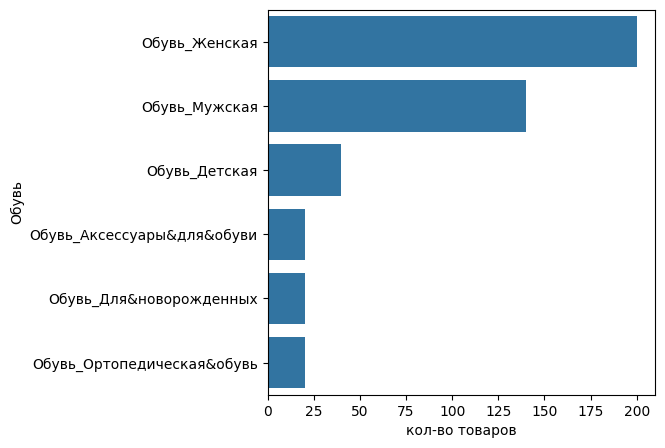
\includegraphics[scale=0.6]{приложения/amount_of_category_Обувь.png}
	\caption{Архитектура дерева классификационных моделей.}
	\label{fig:amount_of_category_Обувь2}
\end{figure}

\begin{table}[ht]
	\caption{Classification report для модели "Обувь".} 
	\label{table:classification_report_example}
	\footnotesize
	\centering
	\begin{tabular}{r|rrrr}
		\toprule
		{} & \multicolumn{1}{c}{precision} & \multicolumn{1}{c}{recall} & \multicolumn{1}{c}{f1-score} & \multicolumn{1}{c}{support}\\
		\midrule
		Обувь\_Аксессуары\&для\&обуви &	1.00 & 0.75 & 0.86 & 4\\
		Обувь\_Детская                & 0.67 & 0.67 & 0.67 & 9\\
		Обувь\_Для\&новорожденных     & 0.33 & 0.33 & 0.33 & 3\\
		Обувь\_Женская                &	0.80 & 0.88 & 0.83 & 40\\
		\bigskip
		Обувь\_Мужская                &	0.76 & 0.68 & 0.72 & 28\\
		accuracy                      &      &      & 0.76 & 84\\
		macro avg                     &	0.71 & 0.66 & 0.68 & 84\\
		weighted avg                  &	0.76 & 0.76 & 0.76 & 84\\
		\bottomrule
	\end{tabular}
\end{table}

\begin{figure}[ht]
	\centering
	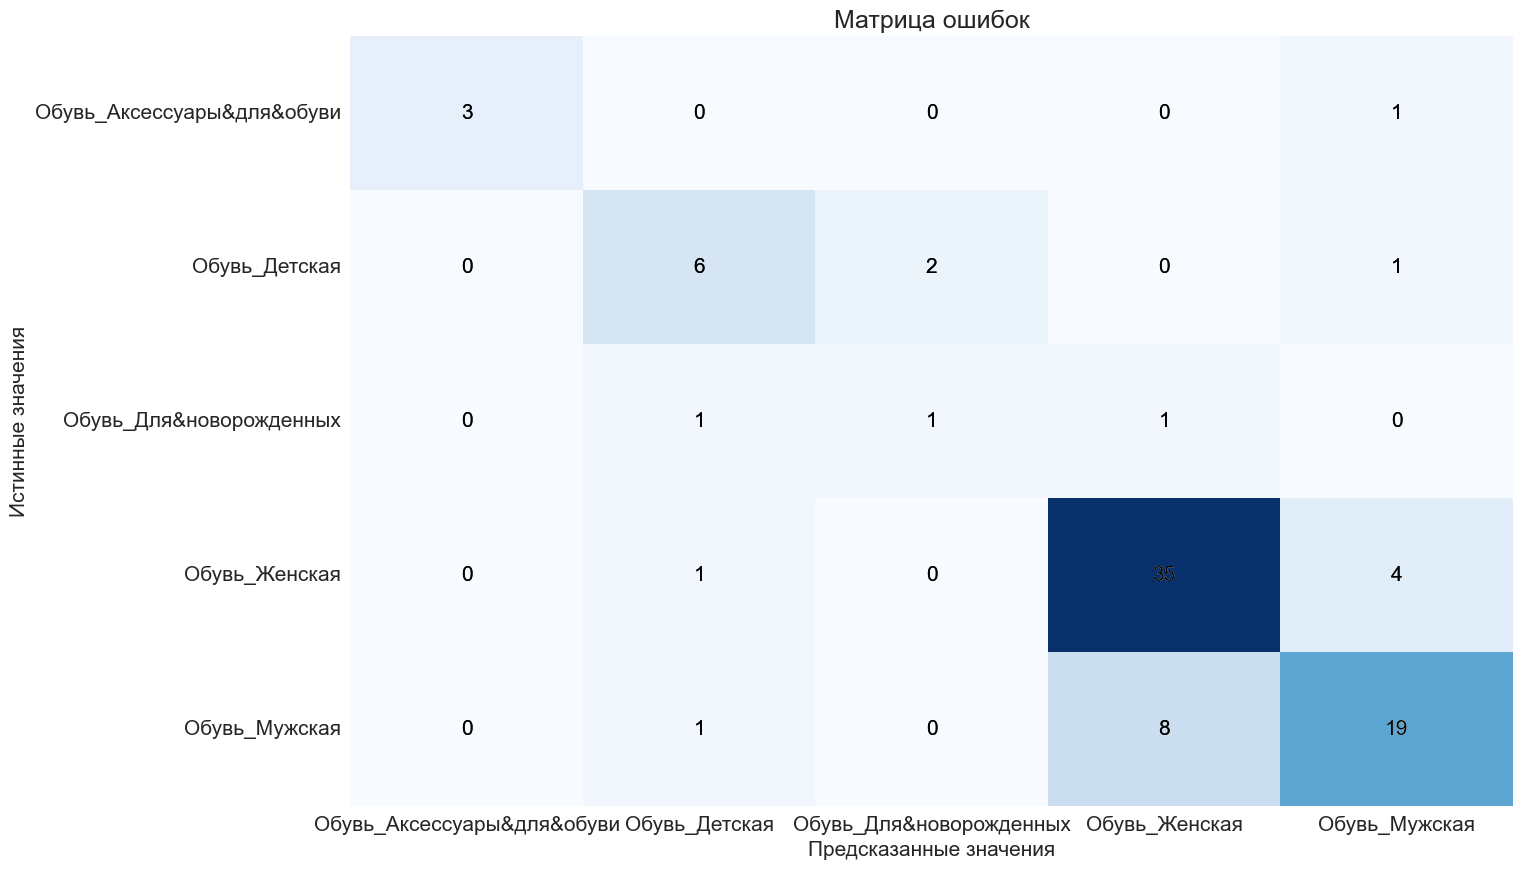
\includegraphics[scale=0.4]{confusion_matrix_shoes.png}
	\caption{Матрица ошибок модели "Обувь" для тестового набора данных}
	\label{fig:confusion_matrix_shoes}
\end{figure}

\begin{table}[ht]
	\caption{Метрики качества модели "Обувь".}
	\label{table:metrics_shoes}
	\footnotesize
	\centering
	\begin{tabular}{l|l}
		\toprule
		\multicolumn{1}{c|}{metric} & \multicolumn{1}{c}{value}\\
		\midrule
		accuracy      & 0.7619\\
		accuracy@top2 & 0.8929\\
		precision     & 0.7111\\
		recall        & 0.6607\\
		f1            & 0.6815\\
		\bottomrule
	\end{tabular}
\end{table}


Для начала стоит принять во внимание, что категория малочисленна и содержит 440 товаров. При разделении на обучающую и тестовую выборки для тестовой было отделено 20\% от всех товаров из категории. Другими словами, часть категорий имела менее 5 примеров в тестовом наборе данных. Легко ожидать, что при небольшом размере категории (например, категория «Обувь\_Для\&новорожденных» включает всего 13 товаров) фотографии товаров могут иметь разнообразный характер, так что в тестовый набор могут попасть фотографии совершенно отличные от обучающего набора. В таком случае не стоит ожидать, что модель, видевшая порядка 10 примеров, сможет распознать данную категория на совершенно отличных по внешнему виду товарах.

Другим важным наблюдением будет достаточно сильная путаница моделью товаров из категорий «Обувь\_Женская» и «Обувь\_Мужская». Проанализировав собранные данные и согласно здравому смыслу, легко заметить, что некоторые женские и мужские модели обуви похожи. Особенно сложно отличить обувь из подкатегории «Кеды\&и\&кроссовки». Для наглядности на рисунке \ref{fig:classification_exampleshoes} представлены товары из подкатегории «Кеды\&и\&кроссовки» для женщин (слева) и мужчин (справа). Аналогичный вывод справедлив и для категории «Обувь\_Детская», где можно найти похожие взрослую обувь модели.

\begin{figure}[ht]
	\centering
	\begin{minipage}[b]{3in}
		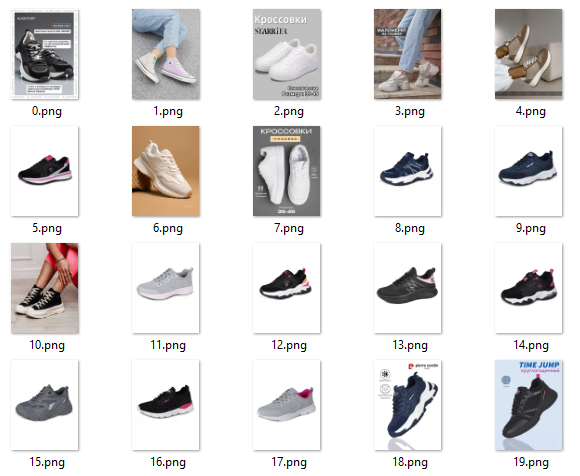
\includegraphics[scale=0.5]{classification/classification_exampleshoes1.png}
		%		\caption{Изображения, попавшие в категорию "Обувь\_Женская\_Кеды\&и\&кроссовки".}
		%		\label{fig:classification_exampleshoes1}
	\end{minipage}
	\hfill
	\begin{minipage}[b]{3in}
		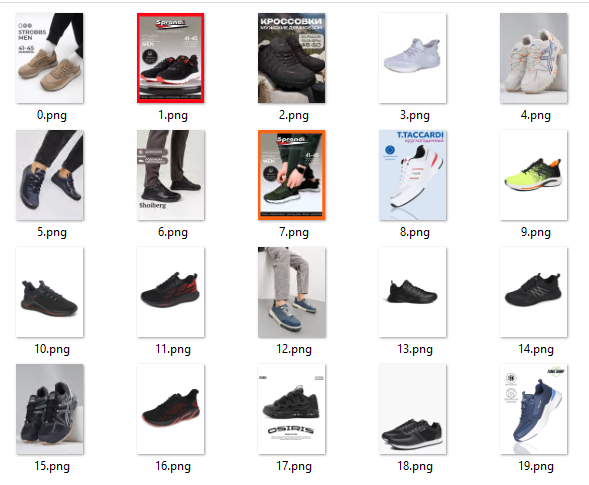
\includegraphics[scale=0.5]{classification/classification_exampleshoes2.png}
		%		\caption{Изображения, попавшие в категорию "Обувь\_Мужская\_Кеды\&и\&кроссовки".}
		%		\label{fig:classification_exampleshoes2}
	\end{minipage}
	\caption{Изображения, попавшие в категорию "Обувь\_Женская\_Кеды\&и\&кроссовки" (слева) и  категорию "Обувь\_Мужская\_Кеды\&и\&кроссовки" (справа).}
	\label{fig:classification_exampleshoes}
\end{figure}

Последним важным замечание относительно особенностей данных будет наличие неудачного парсинга в некоторых случаях, которое невозможно заранее предугадать. Так, например, в категории «Обувь\_Для\&новорожденных» в момент сбора данных попались неудачные товары (см. сравнение товаров \ref{fig:classification_exampleshoes2}, размещенных на «Wildberris» на текущий момент, и попавших в собранную выборку), которые предположительно впоследствии отчасти были перенесены в другую категорию работниками «Wildberries» либо претерпели другие изменения. Можно заметить, что хотя категория предполагает обувь для новорожденных, по собранным с ней товарам тематика ставится под сомнение. Например, очень много присутствует товаров, таких как балетки или внешне более взрослые кроссовки, которые с таким же успехом можно было отнести к категории «Обувь\_Детская» и в которой действительно присутствуют подобные товары.

\begin{figure}[ht]
	\centering
	\begin{minipage}[b]{3in}
		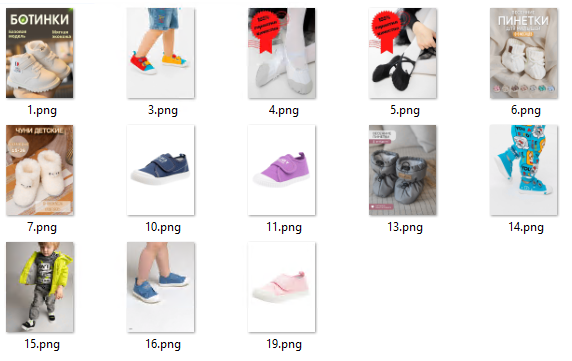
\includegraphics[scale=0.5]{classification/classification_exampleshoes3.png}
	\end{minipage}
	\hfill
	\begin{minipage}[b]{3in}
		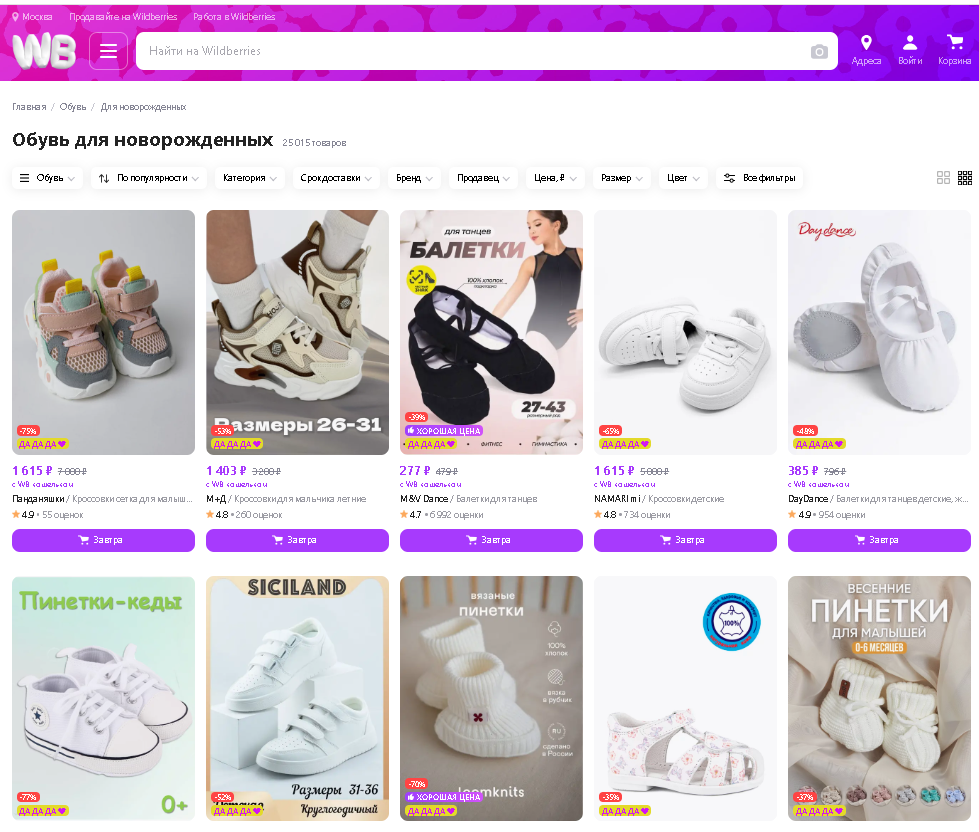
\includegraphics[scale=0.25]{classification/classification_exampleshoes4.png}
	\end{minipage}
	\caption{Изображения, попавшие в категорию "Обувь\_Для\&новорожденных" при парсинге (слева) и пример товаров, размещенных в разделе "Обувь\_Для\&новорожденных" на текущий момент на "Wildberries" (справа).}
	\label{fig:classification_exampleshoes2}
\end{figure}

Из всего вышеперечисленного, а также из замечаний, описанных в разделе \ref{classification_metrics}, следует главным образом один вывод – ожидать от модели классификации качества близкого к идеальному не стоит. Такова действительность работы с реальными данными, подверженными законам реальной жизни. На рисунке \ref{fig:classification_errorshoes} представлены некоторые из ошибок классификатора на тестовых данных.

\begin{figure}[ht]
	\centering
	\begin{minipage}[b]{1.2in}
		
\includegraphics[scale=0.4]{classification/classification_errorshoes1.png}
	\end{minipage}
	\hfill
	\begin{minipage}[b]{0.8in}
		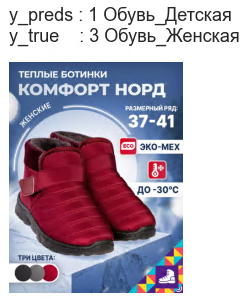
\includegraphics[scale=0.4]{classification/classification_errorshoes2.png}
	\end{minipage}
	\hfill
	\begin{minipage}[b]{1.1in}
		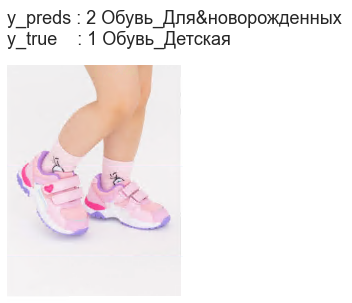
\includegraphics[scale=0.4]{classification/classification_errorshoes3.png}
	\end{minipage}
	\hfill
	\begin{minipage}[b]{0.8in}
		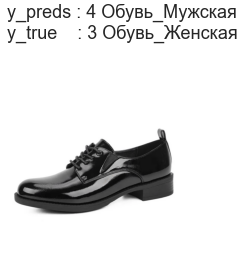
\includegraphics[scale=0.4]{classification/classification_errorshoes4.png}
	\end{minipage}
	\hfill
	\begin{minipage}[b]{1in}
		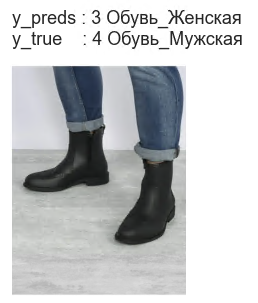
\includegraphics[scale=0.4]{classification/classification_errorshoes5.png}
	\end{minipage}
	\caption{Примеры изображений из тестового набора даных, на которых был предсказан неверный класс (y\_preds - класс, предсказанный моделью, y\_true - инстиный класс).}
	\label{fig:classification_errorshoes}
\end{figure}

Проведем анализ PR и ROC кривых (см. рисунок \ref{fig:prcurve_Обувь2} и \ref{fig:roccurve_Обувь2} соответственно). В поведении кривых с макро и микроусреднением по классам можно заметить картину, аналогичную кривым, объединенным по всем моделям. В рассуждении стоит отталкиваться в первую очередь от анализа порогов отсечения, используемых для построения PR-кривых, и распределения плотности значений на графиках. 

\begin{figure}[ht]
	\centering
	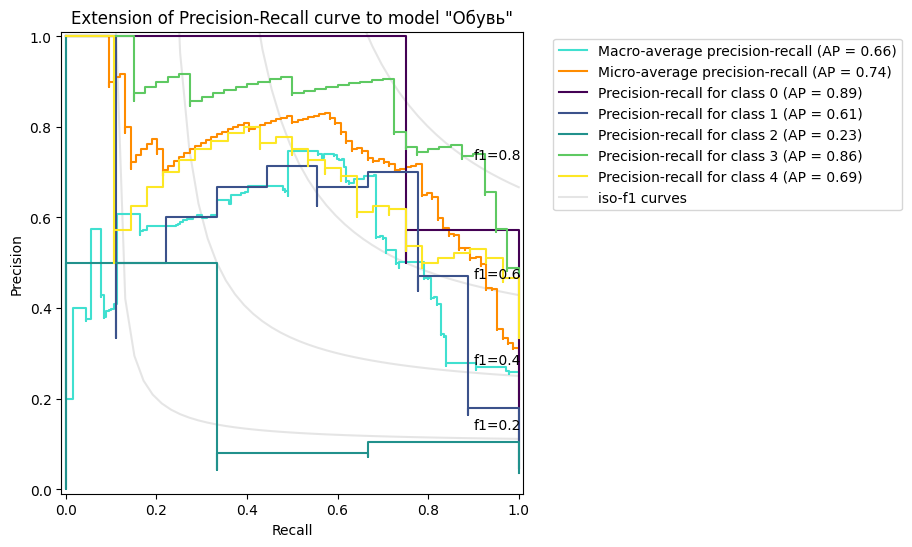
\includegraphics[scale=0.6]{pr_curves/prcurve_Обувь.png}
	\caption{PR-curve для модели "Обувь".}
	\label{fig:prcurve_Обувь2}
\end{figure}

На голубой кривой, отвечающей за макроусреднение, при наивысших порогах отсечения имеется виденное ранее «проседание» в качестве precision. Это происходит по двум причинам. В таблице \ref{table:quantile_shoes} представлены квантили порогов отсечения выше 0.9 для данной кривой. В 90\% случаях вероятности предсказаний модели меньше 0.5. Такой показатель говорит о еще более неуверенной классификации, чем в общем случае. Другой причиной является особенности данных, которые влияют в том числе и на качество классификатора. В категории «Обувь» наименее хорошо предсказывается класс «Обувь\_Для\&новорожденных» (см. таблицы \ref{table:classification_report_example} - \ref{table:metrics_shoes}), что соответствует второму классу\footnote{Подобная достаточно сильная неуверенность классификатора проявляется и в других классах.}. Из таблицы верхних квантилей порогов отсечения (см. таблицу \ref{table:quantile_shoescat2}) видно, что максимальная вероятность на тестовых примерах в данной категории равняется 0.58, что является очень низким значением. Девяносто девятый квантиль составляет 39\%. То есть классификатор на данной категории очень не уверен и с трудом отличает ее от других. Принимая во внимание способ расчета метрик при макроусреднении, который усредняет значение показателей precision и recall по всем классам, неудивительно падение preсision на высоких порогах отсечения.

\begin{table}[ht]
	\footnotesize
	\begin{minipage}[t]{0.5\textwidth}
	\centering
	\begin{tabular}{cc}
		\toprule
		\multicolumn{1}{c}{quantile} & \multicolumn{1}{c}{threshold}\\
		\midrule
		0.90 & 0.476\\
		0.91 & 0.501\\
		0.92 & 0.513\\
		0.93 & 0.535\\
		0.94 & 0.585\\
		0.95 & 0.604\\
		0.96 & 0.629\\
		0.97 & 0.648\\
		0.98 & 0.695\\
		0.99 & 0.772\\
		1.00 & 0.858\\
		\bottomrule
	\end{tabular}
	\captionof{table}{Верхние квантили вероятностных порогов, участвовавших в построении PR-кривых модели "Обувь".}
	\label{table:quantile_shoes}
	\end{minipage}
	\begin{minipage}[t]{0.5\textwidth}
	\centering
	\begin{tabular}{cc}
		\toprule
		\multicolumn{1}{c}{quantile} & \multicolumn{1}{c}{threshold}\\
		\midrule
		0.90 & 0.476\\
		0.91 & 0.501\\
		0.92 & 0.513\\
		0.93 & 0.535\\
		0.94 & 0.585\\
		0.95 & 0.604\\
		0.96 & 0.629\\
		0.97 & 0.648\\
		0.98 & 0.695\\
		0.99 & 0.772\\
		1.00 & 0.858\\
		\bottomrule
	\end{tabular}
	\captionof{table}{Верхние квантили вероятностных порогов, участвовавших в построении PR-кривой для категории «Обувь\_Для\&новорожденных» модели "Обувь".}	
	\label{table:quantile_shoescat2}
	\end{minipage}
\end{table}

Подобное проседание метрики precision и параболообразная форма кривой заметно и на оранжевой линии, отвечающей за микроусреднение метрик, с тем различием, что падение качества происходит не сразу. Отдаление падения значения precision можно объяснить тем, что, принимая во внимание принцип расчета микро метрик и низкие вероятности предсказаний на некоторых категорий, классификация получается очень точной (precision равен 1). Как только происходит понижение порога до уровня, когда в игру вступают плохо предсказываемые категории или неоднозначные фотографии, возникает взлет false positive примеров и проседание preсision.

Таким образом, исходя из визуального и аналитического анализа кривых, наиболее удачным выбором порога будут пороги, соответствующие вершинам парабол micro-average и macro-average pr-curve (оранжевая и голубая линии соответственно). Данный фрагмент характеризует 0.35-0.37 вероятностные пороги, при которых precision варьируется в диапазоне 74-73\%, а recall находится в районе 59\%.

\begin{figure}[h]
	\centering
	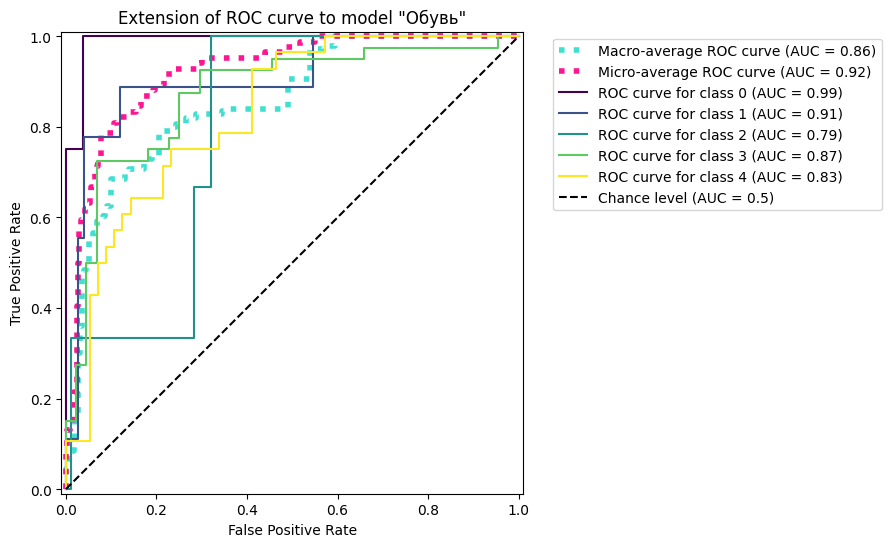
\includegraphics[scale=0.6]{roc_curves/roccurve_Обувь.png}
	\caption{ROC-curve для модели "Обувь".}
	\label{fig:roccurve_Обувь2}
\end{figure}

Показатели ROC кривых (см. рисунок \ref{fig:roccurve_Обувь2}) согласуются со всеми вышеприведенными выводами. В целом значение AUC по классам довольно неплохое (ожидаемо, самое низкое в категории «Обувь\_Для\&новорожденных», класс 2), все значения превышают показатель в 80\%.

Подытоживая анализ модели, построенной на категорию «Обувь», можно сказать, что в модели присутствуют как хорошо-, так и плохопредсказываемые классы. В связи с этим, при оценивании модели в целом при макроусреднении показатели получаются более низкими, поскольку все классы имеют одинаковую важность. При микроусреднении метрик по классам картина более оптимистичная, так как плохая предсказательная сила на малочисленных классах нивелируется хорошими показателями на многочисленных категориях.


\subsection{Решение задачи создания подписей к изображениям}

После обучения всех классификаторов и получения из них эмбедингов изображений можно было переходить к решению задача генераций текстового описания. 

Первым этапом в решении задачи создания подписей к изображениям стала подготовка собранных с «Wildberries» текстов. К данному вопросу стоит отнестись с особой осторожностью, поскольку внешний вид текстов, поданных в модель, будет напрямую влиять на полученные из нее описания. Существует большое разнообразие вариантов предобработки текстовых данных, способствующих улучшению производительности модели, таких как удаление лишних символов и стоп-слов, приведение к нижнему регистру, лемматизация и стемминг, обработка чисел и дат, токенизация и другие. Выбор пайплайна предварительной обработки зависит от поставленной задачи и требований, выдвигаемых к тексту. В рамках данной работы к текстам было поставлено следующее условие – генерируемые моделью тексты должны быть максимально похожими на настоящие тексты. Исходя из этого все цифры, специальные символы, знаки препинания и связующие частицы были оставлены без изменений, так как они способствуют сохранению важных структурных и семантических особенностей текста. Прочая обработка заключалась в приведении всех символов к нижнему регистру, для сокращения итогового числа токенов. График \ref{fig:captions_length} содержит статистику по длинам последовательностей, полученных после предобработки. Можно заметить, что чаще всего размер описания не превосходит 2000 символом, что соответствует примерно 400 словам\footnote{Расчет исходит из средней длины слова в 5 букв.}. Максимальная встречаемая длина равнялась 5000 символам, то есть примерно 1000 словам. Авторами было принято решение не ставить сильных ограничений на длину последовательности и производить при необходимости обрезку текста по 5000 символам.
\begin{figure}[ht]
	\centering
	\includegraphics[scale=0.7]{captions_length.png}
	\caption{Распределение длин описаний товаров. \textsl{Примечание:} длины рассчитаны в символах.}
	\label{fig:captions_length}
\end{figure}
Затем была применены алгоритмы токенизации текста в двух вариантах.

Токенизатор - это ключевой компонент в процессе обработки текста, который разбивает текст на отдельные токены или слова. Выбор подходящего токенизатора существенно влияет на результат генерации текста в моделях обработки естественного языка и является критически важным шагом.

Для генерации текста были опробованы и применены следующие токенизаторы:
\begin{itemize}
	\item Кодирование парами байтов (от англ.Byte Pair Encoding, BPE) — это один из самых популярных методов токенизации, основанный на статистическом анализе корпуса текстов. Токенизатор разбивает текст на наименьшие семантически значимые подстроки, называемые байт-парами, что обеспечивает эффективную обработку редких слов и подслов. Это особенно полезно при генерации текста, где важно учитывать различные варианты слов и их частотность. Поскольку BPE работает на уровне байтов или подслов, ему нужно больше данных для эффективного построения словаря и выделения семантически значимых токенов. Это особенно важно для работы с редкими или нестандартными словами. BPE может быть более гибким и эффективным в обработке текста, но он также более сложен в настройке и требует больше вычислительных ресурсов. Тем не менее, при правильной настройке он может обеспечить более точное и гибкое представление текста.
	\item Токенизатор на уровне слов (от англ. Word Level Tokenizer) - это метод токенизации, который разбивает текст на отдельные слова или токены на основе пробелов или других разделителей. В отличие от BPE, который может разбивать текст на более мелкие подстроки и тем самым учитывать подслова или суффиксы, токенизатор на уровне слов работает на уровне целых слов. Это может привести к потере некоторой семантической информации, особенно в случае сложных слов или словоформ.
\end{itemize}
При неограниченном размере словаря число токенов равнялось примерно 160 тыс. в случае BPE токенизатора и 130 тыс. в случае Wordlevel токенизатора.

Было придумало несколько вариантов моделей с постепенным усложнением ее архитектуры. Во всех предложенных модификациях тестировались LSTM и GRU блоки.

Бейзлайном выступил одиночный блок рекуррентной сети (см. рисунок \ref{fig:rnn_one}).
\begin{figure}[ht]
	\centering
	\includegraphics[scale=0.7]{rnn_one.png}
	\caption{Cхема генерации текста при помощи одного блока RNN.}
	\label{fig:rnn_one}
\end{figure}
Следующим усложнение схемы было добавление последовательных блоков RNN, в которых выход предыдущего блока становится входом последующего (см. рисунок \ref{fig:rnn-multilayer}).
\begin{figure}[ht]
	\centering
	\includegraphics[scale=0.7]{rnn-multilayer.png}
	\caption{Cхема генерации текста при помощи последовательных блоков RNN.}
	\label{fig:rnn-multilayer}
\end{figure}
Далее был предложен вариант реализации параллельных RNN с двумя вариациями получения предсказаний (см. рисунок \ref{fig:rnn-parallel-concatenation}, \ref{fig:rnn-parallel-weighted}): конкатенация и взвешивание. При параллельных RNN эмбединг изображения прогоняется одновременно через несколько блоков multi-layer RNN (см. рисунок \ref{fig:rnn-multilayer}) по принципу сиамских моделей. В варианте конкатенации к выходам из multi-layer RNN блоков применяется конкатенация с последующим навешиванием на полученный тензор линейного слоя для получения предсказания. В варианте со взвешиванием выходы multi-layer RNN блоков перевзвешиваются с определенными весами, аналогично наложению линейной регрессии. После на полученный тензор также накладывается линейный слой.
\begin{figure}[ht]
\begin{minipage}[b]{3in}
	\includegraphics[scale=0.5]{rnn-parallel-concatenation.png}
	\caption{Параллельные RNN (конкатенация).}
	\label{fig:rnn-parallel-concatenation}
\end{minipage}
\hfill
\begin{minipage}[b]{3in}
	\includegraphics[scale=0.5]{rnn-parallel-weighted.png}
	\caption{Параллельные RNN (взвешивание).}
	\label{fig:rnn-parallel-weighted}
\end{minipage}
\end{figure}
Последней предложенной модификацией стало добавление двух видов attention (подробнее ок каждом см. в разделе \ref{subsection:image-captioning}):
\begin{itemize}
	\item взвешенное внимание;
	\item механизм внимания, который позволяет модели сосредоточиться на различных частях изображения с разной степенью важности на каждом этапе генерации.
\end{itemize}

Из анализа результатов классификационного дерева была выдвинута гипотеза, что качество классификации может оказывать влияние на качество сформированного эмбединга изображения и, следовательно, качество генерации текстовых описаний. Принимая во внимание разницу в качестве классификаций на обучающем и тестовом наборе данных\footnote{Разделение собранных данных на обучающую и тестовую выборки было произведено один раз в самом начале. Таким образом, тестовые данные для задачи классификации и для задачи генерации текстовых описаний были одними и теми же.}, было предложено отделить от обучающего датасета небольшое количество данных\footnote{Будем называть отделенную часть валидационным набором данных.} (15\%), примерно равное тестовому датасету, которое впоследствии отражало бы качество генераций на эмбедингах изображений, полученных из уверенного классификатора (см. таблицу \ref{table:image-caption-dataset-size}). Таким образом, способность модели генерировать описания проверялась в трех вариантах: обучающий набор данных отражал данные, которые модель видела при обучении (отсутствие ошибки модели), валидационный – данные при условии хорошей классификации, но которые модель не видела при обучении (ошибка модели генерации), тестовый – данные при условии не очень качественной классификации и которые модель тоже не видела при обучении (наложение ошибок модели классификации и генерации).

\begin{table}[ht]
	\caption{Размеры датасетов для задачи генерации подписей к изображениям.}
	\label{table:image-caption-dataset-size}
	\footnotesize
	\centering
	\begin{tabular}{l|l}
		\toprule
		{} & \multicolumn{1}{c}{dataset size}\\
		\midrule
		train dataset & 18857\\
		val dataset   & 3329\\
		test dataset  & 5550\\
		\bottomrule
	\end{tabular}
\end{table}

При генерации текста для выбора наиболее вероятных последовательности слов использовались следующие стратегии (подробнее о каждой см. в разделе \ref{schema-gen-text}):
\begin{itemize}
	\item жадный поиск;
	\item категориальная выборка;
	\item beam search.
\end{itemize}

На рисунках \ref{fig:test-rnn-glass-1}, \ref{fig:test-rnn-glass-2}, \ref{fig:test-rnn-art-1} и \ref{fig:test-rnn-art-2} представлены примеры генерации текста для товаров с тремя стратегиями выбора наиболее вероятных последовательности слов. Подсчитаны метрик WER и BLEU.

\begin{figure}[ht]
	\centering
	\includegraphics[scale=0.4]{test-rnn-glass-1.png}
	\caption{Cхема генерации текста для очков. Часть 1.}
	\label{fig:test-rnn-glass-1}
\end{figure}

\newpage
\begin{figure}[ht]
	\centering
	\includegraphics[scale=0.4]{test-rnn-glass-2.png}
	\caption{Cхема генерации текста для очков. Часть 2.}
	\label{fig:test-rnn-glass-2}
\end{figure}

\newpage
\begin{figure}[ht]
	\centering
	\includegraphics[scale=0.4]{test-rnn-art-1.png}
	\caption{Cхема генерации текста для набора для творчества. Часть 1.}
	\label{fig:test-rnn-art-1}
\end{figure}

\newpage
\begin{figure}[ht]
	\centering
	\includegraphics[scale=0.4]{test-rnn-art-2.png}
	\caption{Cхема генерации текста для набора для творчества. Часть 2.}
	\label{fig:test-rnn-art-2}
\end{figure}

В ходе проведенного анализа генерации текста, можно сделать следующие выводы:
\begin{enumerate}[label=\arabic*.]
	\item Beam Search обеспечивает наилучшее качество генерации текста, создавая более семантически и грамматически правильные предложения. Эта стратегия позволяет учитывать несколько наиболее вероятных путей развития текста, что значительно улучшает итоговое качество по сравнению с другими методами.
	\item Жадный поиск, хотя и эффективен по времени, может упускать более качественные варианты текста из-за склонности попадать в локальные минимумы, что можно заметить на примере \ref{fig:test-rnn-art-1} генерации текста для набора для творчества. Это означает, что, выбирая на каждом шаге только наиболее вероятное слово, он может упустить более качественные и смысловые варианты, которые могли бы быть достигнуты при учете альтернативных путей.
	\item Категориальная выборка, несмотря на создание более длинных текстов, часто страдает от недостаточной связности и осмысленности содержания.
\end{enumerate}

В результате проведенных экспериментов была проверена гипотеза о том что качество, качество классификации влияет на качество генерации описания.

Стоит отметить, что при генерации текста неплохо было бы учитывать ключевые слова. Включение ключевых слов позволит сделать текст более целенаправленным и релевантным, что особенно важно для описания товаров.

\newpage
\newpage
\section{Проектирование архитектуры программного продукта}
В 2022 году граждане Российской Федераций столкнулись с трудностями работы с магазинами приложений для смарт-устройств. Так, например, с 24 февраля из российского раздела App Store были удалены почти 7000 мобильных приложений \cite{russiaapp}. Поэтому при построении архитектуры приложения был выбран подход к созданию клиент-серверного приложения, которое будет работать практически на любом устройстве (стационарный компьютер, ноутбук, планшет или смартфон). Одним из способов реализации такого подхода является написание telegram  бота. В настоящее время это одно из трендовых направлений в IT сфере. В 2024 году Telegram посещают 900 миллионов человек в месяц \cite{telegram-stats}. По количеству аудитории он входит в пятерку самых популярных мессенджеров в мире. Выбор в пользу написания телеграм-бота вместо веб-приложения может быть обусловлен рядом факторов, включая удобство использования, скорость разработки, доступность, безопасность, а также гибкость и масштабированность для обработки большого количества пользователей.

За логику, работоспособность и правильное функционирование бота 
отвечает серверная часть (англ. backend), которая скрыта от пользователя. Серверная часть включает в себя:
\begin{itemize}
	\item модуль для обработки запросов от пользователя;
	\item модуль для взаимодействия с обученной моделями классификации для определения категории товара и генерации его описания.
\end{itemize}

В контексте работы с моделями машинного обучения и их применения в системах автономного управления, вынос предсказаний моделей в очередь сообщений может быть полезно для оптимизации работы и повышения устойчивости системы.

На рисунке \ref{fig:app-arch} представлена архитектура программного продукта с использованием стека технологий (подробнее см. в разделе \ref{stack-tech}).

\begin{figure}[ht]
	\centering
	\includegraphics[scale=0.5]{app-arch.png}
	\caption{Архитектура ПО с использованием стека технологий.}
	\label{fig:app-arch}
\end{figure}


\subsection{Стек технологий}\label{stack-tech}
Для проектирования, разработки и обучения нейронных сетей использовался следующий стек технологий:
\begin{itemize}
	\item Язык программирования Python — язык общего назначения, с помощью которого можно решать сложные задачи машинного обучения и быстро создавать прототипы для последующей их отладки. Язык гибкий и мультиплатформенный, имеет обширный набор библиотек для искусственного интеллекта. Python удобно использовать для обработки и подготовки обучающих данных \cite{pyton}.
	\item Для реализации архитетуры нейронной сети использовался Pytorch — библиотека глубокого обучения с открытым исходным кодом, написанная на языке Python и созданная на базе Torch. Используется для решения различных задач машинного обучения: компьютерное зрение, NLP, создания и обучения нейронных сетей \cite{pytorch}. Простота использования, обширные возможности и активное сообщество делают ее популярным выбором для исследования и разработки в области глубокого обучения.
	\item Для реализация серверной части был выбран FastAPI – это современный и быстрый фреймворк для создания веб-приложений на языке Python, предлагающий полезные инструменты и функции для облегчения процесса создания веб-приложений\cite{fastapi}.
	\item При реализации механизма обработки очереди задач использовалась комбинация инструментов: Celery\cite{celery} и RabbitMQ\cite{rabbitmq} для надежного обмена данными, а также Flower для мониторинга процесса выполнения задач. Celery представляет собой асинхронную очередь задач на языке Python, обеспечивающую создание, планирование и выполнение задач асинхронно. RabbitMQ, в свою очередь, является популярным брокером сообщений для обмена данными между различными компонентами приложения, обеспечивая надежную доставку сообщений и поддерживая различные протоколы и архитектуры коммуникации. Flower представляет собой веб-интерфейс для мониторинга и управления задачами, запущенными с помощью Celery, предоставляя удобную панель управления для отслеживания статуса выполнения задач, просмотра логов и управления очередями. Эта связка обеспечивает гибкое и масштабируемое решение для управления задачами в приложении.
	\item Для хранения информации о пользователях и фотографиях товара используется СУБД PostgreSQL \cite{postgresql}. Она предоставляет надежное хранение данных, поддерживает множество расширений и функций, дает возможность работы с различными типами данных, а также обладает отличной производительностью и масштабируемостью.
	\item Для реализации бота для телеграма используется библиотека Aiogram\cite{aiogram}, которая предоставляет удобные инструменты для работы с API Telegram, обеспечивая простоту в использовании и расширяемость. К преимуществом данной библиотеки можно отнести ассинхронную поддержку кода, наличие работы с медиафайлами, командами, встроенными клавиатурами, опросами и многое другое, что позволяет создавать ботов с различным функционалом.
	\item Для локального тестирования приложения использовался Docker Compose\cite{docker}, что позволило быстро развернуть локальное окружение с минимальными усилиями. Параллельно, для управления контейнеризированным приложением в продукционной среде использовался Kubernetes (k8s)\cite{kubernetes}. Этот выбор обеспечил высокую доступность и масштабируемость приложения.
	Использование Docker Compose и Kubernetes существенно упростило процесс развертывания и повысило качество сервиса, обеспечив надежную и масштабируемую инфраструктуру.
	\item В Docker Compose добавлен мониторинг сервиса с помощью Prometheus\cite{prometheus} и Grafana\cite{grafana}.
\end{itemize}

Вычисления происходили с использованием аппаратных ускорений на GPU Nvidia Tesla V100 и A100.

\subsection{Демонстрация работы приложения}

Чтобы воспользоваться функционалом бота пользователю необходимо ввести команду «/predict» и загрузить фотографию товара. Далее ему будет предложена наиболее вероятная категория товара и сгенерировано SEO-описание. Кроме того, у пользователя будет запрошено подтверждение или отклонение предложенной категории товара. Если пользователю категория не понравится, то бот не будет генерировать описание и попросит перефотографировать товар. В последствии эта обратная связь может быть использована для дообучения модели с целью ее дальнейшего улучшения точности и качества предсказаний.

На рисунках \ref{fig:telegram-jeans-menu} и \ref{fig:telegram-jeans-description} представлены примеры работы сервиса на мужских джинсах.

\begin{figure}[ht]
	\begin{minipage}[b]{3in}
		\centering
		\includegraphics[scale=0.35]{telegram-jeans-menu.png}
		\caption{Демонстрация работы — подтверждение категории.}
		\label{fig:telegram-jeans-menu}
	\end{minipage}
	\hfill
	\begin{minipage}[b]{3in}
		\centering
		\includegraphics[scale=0.35]{telegram-jeans-description.png}
		\caption{Демонстрация работы — генерация описания.}
		\label{fig:telegram-jeans-description}
	\end{minipage}
\end{figure}

\newpage

На рисунке \ref{fig:telegram-parf-description} представлен пример работы сервиса на духах.

\begin{figure}[ht]
	\centering
	\includegraphics[scale=0.35]{telegram-parf-description.png}
	\caption{Демонстрация работы сервиса на духах.}
	\label{fig:telegram-parf-description}
\end{figure}

\newpage

\newpage
\section*{Заключение}
\addcontentsline{toc}{section}{Заключение}

В рамках выпускной квалификационной работы было разработано программное обеспечение, в основе которого реализована модель нейронной сети, способная классифицировать товары на маркетплейсе на основе их фотографий и генерировать соответствующие к ним описания. Формализованы входные и выходные данные.

Были решены все поставленные задачи:
\begin{itemize}
	\item Подготовлен набор данных, содержащий изображения товаров и соответствующие им категории и текстовые описанияй.
	\item Проанализированы существующие архитектуры нейронных сетей, используемых для классификации изображений и генерации текста. В ходе проведенного анализа была выбрана наиболее подходящая архитектура для решения поставленной задачи.
	\item Обучена спроектированная архитектура на подготовленных данных, а затем была оценена ее эффективность.
	\item Спроектирована архитектура программного обеспечения, описаны основные модули.
	\item Интегрирована модель нейронной сети в сервис.
\end{itemize}

Была проверена работоспособность схемы кодера-декодера с использованием комбинации сверточных нейронных сетей для обработки изображений и рекуррентных нейронных сетей для генерации подписей. В задаче классификации были достигнуты следующие результаты: в среднем по моделям доверять дереву классификации можно на 75\%, при этом находя около 65\% объектов положительного класса в тестовой выборке. Этот показатель далек от идеала, но объясним особенностями датасета.

В задаче генерации описаний была использована CNN из задачи классификации в качестве кодировщика и RNN в качестве декодировщика, с последующим усложнением. Это включало разработку новых решений для повышения качества классификации, использование последовательных и параллельных блоков RNN, а также добавление механизма внимания с разными способами его реализации. Однако качество генерации с использованием RNN остается недостаточно высоким. Для улучшения результатов рекомендуется развернуть экземпляр LLM, например, модель GPT-2. 

Итогом работы стало подтверждение, что предложенная схема кодера-декодера успешно решает поставленную задачу. В результате проведенных экспериментов была подтверждена гипотеза о том, что качество классификации влияет на качество генерации описания, чем точнее модель подберет категорию товара, тем лучше будет его описание. Для дальнейшего повышения качества генерации описаний рекомендуется рассмотреть переход на модели трансформеров, которые требуют значительных вычислительных ресурсов и времени на обучение, но могут обеспечить более высокий уровень результатов. Кроме того, выявилась необходимость в увеличении объема датасета для достижения более высоких показателей качества.

Разработанное программное обеспечение имеет перспективу дальнейшего развития и улучшения:
\begin{itemize}
	\item в качестве кодера и декодера использовать трансформеры;
	\item разработка функционала, позволяющего пользователям задавать ключевые слова, которые будут использоваться нейронной сетью при генерации текстовых описаний товаров;
	\item увеличение глубины подбора наиболее подходящей категории;
	\item увеличение количества данных обучающей выборки для повышения показателей точности;
	\item подключение систем для сбора метрик продукта;
	\item рассмотреть другие маркетплейсы («Ozon», «Яндекс Маркет», «Маркет»).
\end{itemize}

\newpage
\section*{Структура деления задач между участниками проекта}
\addcontentsline{toc}{section}{Распределение работ}

Для наглядного представления распределения обязанностей в проекте была составлена таблица \ref{work}, которая позволяет структурировано и ясно проследить прогресс работы, определить распределение обязанностей и оценить вклад каждого члена команды в общий результат.

\begin{table}[h]
	\centering
	\begin{tabular}{ |l|l| } 
		\hline
		\textbf{Бузаева С.М.} & \textbf{Куликов Д.А.}  \\ \hline
		Сбор и анализ данных, написание & Реализация Телеграмм бота \\
		функций для работы с датасетом & \\ \hline
		Очистка данных & Очистка данных \\ \hline
		Реализация и обучение моделей  & Обучение моделей  классификаторов\\ 
		классификаторов  & \\ \hline
		Реализация и обучение моделей RNN & Реализация и обучение моделей RNN \\
		c использованием последовательных & с использованием механизма внимания \\
		и параллельных блоков &  \\ \hline
		Генерация последовательностей &  \\ 
		с помощью Beam Search  &  \\ \hline
		Построение бизнес кривых  &  \\  
		\hline
	\end{tabular}
	\caption{Распределение обязанностей.}
	\label{work}
\end{table}

Процесс разработки программного обеспечения осуществлялся совместными усилиями с использованием gihub-репозитория \cite{github}, который облегчил совместную работу над проектом, управление исходным кодом и процессом разработки, а также повысил эффективность и прозрачность работы всей команды.

\newpage
\nocite{*}
\printbibliography[heading=bibintoc]

\newpage
\appendix

\section{Приложение 1}
\label{appendix:amount_of_categor2}
\textbf{\large{Распределение данных по категориям второй вложенности.}}

\begin{figure}[hbtp]
	\centering
	\includegraphics[scale=0.8]{приложения/amount_of_category_Автотовары.png}
	\caption{Распределение данных в категории «Автотовары».}
	\label{fig:amount_of_category_Автотовары}
\end{figure}

\begin{figure}[hbtp]
	\centering
	\includegraphics[scale=0.8]{приложения/amount_of_category_Аксессуары.png}
	\caption{Распределение данных в категории «Аксессуары».}
	\label{fig:amount_of_category_Аксессуары}
\end{figure}

\begin{figure}[hbtp]
	\centering
	\includegraphics[scale=0.8]{приложения/amount_of_category_Бытовая&техника.png}
	\caption{Распределение данных в категории «Бытовая\&техника».}
	\label{fig:amount_of_category_Бытовая&техника}
\end{figure}

\begin{figure}[hbtp]
	\centering
	\includegraphics[scale=0.8]{приложения/amount_of_category_Детям.png}
	\caption{Распределение данных в категории «Детям».}
	\label{fig:amount_of_category_Детям}
\end{figure}

\begin{figure}[hbtp]
	\centering
	\includegraphics[scale=0.8]{приложения/amount_of_category_Для&ремонта.png}
	\caption{Распределение данных в категории «Для\&ремонта».}
	\label{fig:amount_of_category_Для&ремонта}
\end{figure}

\begin{figure}[hbtp]
	\centering
	\includegraphics[scale=0.8]{приложения/amount_of_category_Дом.png}
	\caption{Распределение данных в категории «Дом».}
	\label{fig:amount_of_category_Дом}
\end{figure}

\begin{figure}[hbtp]
	\centering
	\includegraphics[scale=0.8]{приложения/amount_of_category_Женщинам.png}
	\caption{Распределение данных в категории «Женщинам».}
	\label{fig:amount_of_category_Женщинам}
\end{figure}

\begin{figure}[hbtp]
	\centering
	\includegraphics[scale=0.8]{приложения/amount_of_category_Здоровье.png}
	\caption{Распределение данных в категории «Здоровье».}
	\label{fig:amount_of_category_Здоровье}
\end{figure}

\begin{figure}[hbtp]
	\centering
	\includegraphics[scale=0.8]{приложения/amount_of_category_Зоотовары.png}
	\caption{Распределение данных в категории «Зоотовары».}
	\label{fig:amount_of_category_Зоотовары}
\end{figure}

\begin{figure}[hbtp]
	\centering
	\includegraphics[scale=0.8]{приложения/amount_of_category_Игрушки.png}
	\caption{Распределение данных в категории «Игрушки».}
	\label{fig:amount_of_category_Игрушки}
\end{figure}

\begin{figure}[hbtp]
	\centering
	\includegraphics[scale=0.8]{приложения/amount_of_category_Канцтовары.png}
	\caption{Распределение данных в категории «Канцтовары».}
	\label{fig:amount_of_category_Канцтовары}
\end{figure}

\begin{figure}[hbtp]
	\centering
	\includegraphics[scale=0.8]{приложения/amount_of_category_Книги.png}
	\caption{Распределение данных в категории «Книги».}
	\label{fig:amount_of_category_Книги}
\end{figure}

\begin{figure}[hbtp]
	\centering
	\includegraphics[scale=0.8]{приложения/amount_of_category_Красота.png}
	\caption{Распределение данных в категории «Красота».}
	\label{fig:amount_of_category_Красота}
\end{figure}

\begin{figure}[hbtp]
	\centering
	\includegraphics[scale=0.8]{приложения/amount_of_category_Мебель.png}
	\caption{Распределение данных в категории «Мебель».}
	\label{fig:amount_of_category_Мебель}
\end{figure}

\begin{figure}[hbtp]
	\centering
	\includegraphics[scale=0.8]{приложения/amount_of_category_Мужчинам.png}
	\caption{Распределение данных в категории «Мужчинам».}
	\label{fig:amount_of_category_Мужчинам}
\end{figure}

\begin{figure}[hbtp]
	\centering
	\includegraphics[scale=0.8]{приложения/amount_of_category_Обувь.png}
	\caption{Распределение данных в категории «Обувь».}
	\label{fig:amount_of_category_Обувь}
\end{figure}

\begin{figure}[hbtp]
	\centering
	\includegraphics[scale=0.8]{приложения/amount_of_category_Продукты.png}
	\caption{Распределение данных в категории «Продукты».}
	\label{fig:amount_of_category_Продукты}
\end{figure}

\begin{figure}[hbtp]
	\centering
	\includegraphics[scale=0.8]{приложения/amount_of_category_Сад&и&дача.png}
	\caption{Распределение данных в категории «Сад\&и\&дача».}
	\label{fig:amount_of_category_Сад&и&дача}
\end{figure}

\begin{figure}[hbtp]
	\centering
	\includegraphics[scale=0.8]{приложения/amount_of_category_Товары&для&взрослых.png}
	\caption{Распределение данных в категории «Товары\&для\&взрослых».}
	\label{fig:amount_of_category_Товары&для&взрослых}
\end{figure}

\begin{figure}[hbtp]
	\centering
	\includegraphics[scale=0.8]{приложения/amount_of_category_Электроника.png}
	\caption{Распределение данных в категории «Электроника».}
	\label{fig:amount_of_category_Электроника}
\end{figure}

\begin{figure}[hbtp]
	\centering
	\includegraphics[scale=0.8]{приложения/amount_of_category_Ювелирные&изделия.png}
	\caption{Распределение данных в категории «Ювелирные\&изделия».}
	\label{fig:amount_of_category_Ювелирные&изделия}
\end{figure}

\newpage
\section{Приложение 2}
\label{appendix:pr_curves}
\textbf{\large{PR кривые, построенные для каждой классификационной модели.}}

\begin{figure}[hbtp]
	\centering
	\includegraphics[scale=0.7]{pr_curves/prcurve_full_model.png}
	\caption{PR-curves для модели "full\_model".}
	\label{fig:prcurve_full_model}
\end{figure}

\begin{figure}[hbtp]
	\centering
	\includegraphics[scale=0.7]{pr_curves/prcurve_Автотовары.png}
	\caption{PR-curves для модели «Автотовары».}
	\label{fig:prcurve_Автотовары}
\end{figure}

\begin{figure}[hbtp]
	\centering
	\includegraphics[scale=0.7]{pr_curves/prcurve_Аксессуары.png}
	\caption{PR-curves для модели «Аксессуары».}
	\label{fig:prcurve_Аксессуары}
\end{figure}

\begin{figure}[hbtp]
	\centering
	\includegraphics[scale=0.7]{pr_curves/prcurve_Бытовая&техника.png}
	\caption{PR-curves для модели «Бытовая\&техника».}
	\label{fig:prcurve_Бытовая&техника}
\end{figure}

\begin{figure}[hbtp]
	\centering
	\includegraphics[scale=0.7]{pr_curves/prcurve_Детям.png}
	\caption{PR-curves для модели «Детям».}
	\label{fig:prcurve_Детям}
\end{figure}

\begin{figure}[hbtp]
	\centering
	\includegraphics[scale=0.7]{pr_curves/prcurve_Для&ремонта.png}
	\caption{PR-curves для модели «Для\&ремонта».}
	\label{fig:prcurve_Для&ремонта}
\end{figure}

\begin{figure}[hbtp]
	\centering
	\includegraphics[scale=0.7]{pr_curves/prcurve_Дом.png}
	\caption{PR-curves для модели «Дом».}
	\label{fig:prcurve_Дом}
\end{figure}

\begin{figure}[hbtp]
	\centering
	\includegraphics[scale=0.7]{pr_curves/prcurve_Женщинам.png}
	\caption{PR-curve для модели «Женщинам».}
	\label{fig:prcurve_Женщинам}
\end{figure}

\begin{figure}[hbtp]
	\centering
	\includegraphics[scale=0.7]{pr_curves/prcurve_Здоровье.png}
	\caption{PR-curve для модели «Здоровье».}
	\label{fig:prcurve_Здоровье}
\end{figure}

\begin{figure}[hbtp]
	\centering
	\includegraphics[scale=0.7]{pr_curves/prcurve_Зоотовары.png}
	\caption{PR-curves для модели «Зоотовары».}
	\label{fig:prcurve_Зоотовары}
\end{figure}

\begin{figure}[hbtp]
	\centering
	\includegraphics[scale=0.7]{pr_curves/prcurve_Игрушки.png}
	\caption{PR-curves для модели «Игрушки».}
	\label{fig:prcurve_Игрушки}
\end{figure}

\begin{figure}[hbtp]
	\centering
	\includegraphics[scale=0.7]{pr_curves/prcurve_Канцтовары.png}
	\caption{PR-curves для модели «Канцтовары».}
	\label{fig:prcurve_Канцтовары}
\end{figure}

\begin{figure}[hbtp]
	\centering
	\includegraphics[scale=0.7]{pr_curves/prcurve_Красота.png}
	\caption{PR-curves для модели «Красота».}
	\label{fig:prcurve_Красота}
\end{figure}

\begin{figure}[hbtp]
	\centering
	\includegraphics[scale=0.7]{pr_curves/prcurve_Мебель.png}
	\caption{PR-curves для модели «Мебель».}
	\label{fig:prcurve_Мебель}
\end{figure}

\begin{figure}[hbtp]
	\centering
	\includegraphics[scale=0.7]{pr_curves/prcurve_Мужчинам.png}
	\caption{PR-curves для модели «Мужчинам».}
	\label{fig:prcurve_Мужчинам}
\end{figure}

\begin{figure}[hbtp]
	\centering
	\includegraphics[scale=0.7]{pr_curves/prcurve_Обувь.png}
	\caption{PR-curves для модели «Обувь».}
	\label{fig:prcurve_Обувь}
\end{figure}

\begin{figure}[hbtp]
	\centering
	\includegraphics[scale=0.7]{pr_curves/prcurve_Продукты.png}
	\caption{PR-curves для модели «Продукты».}
	\label{fig:prcurve_Продукты}
\end{figure}

\begin{figure}[hbtp]
	\centering
	\includegraphics[scale=0.7]{pr_curves/prcurve_Сад&и&дача.png}
	\caption{PR-curves для модели «Сад\&и\&дача».}
	\label{fig:prcurve_Сад&и&дача}
\end{figure}

\begin{figure}[hbtp]
	\centering
	\includegraphics[scale=0.7]{pr_curves/prcurve_Товары&для&взрослых.png}
	\caption{PR-curves для модели «Товары\&для\&взрослых».}
	\label{fig:prcurve_Товары&для&взрослых}
\end{figure}

\begin{figure}[hbtp]
	\centering
	\includegraphics[scale=0.7]{pr_curves/prcurve_Электроника.png}
	\caption{PR-curves для модели «Электроника».}
	\label{fig:prcurve_Электроника}
\end{figure}

\begin{figure}[hbtp]
	\centering
	\includegraphics[scale=0.7]{pr_curves/prcurve_Ювелирные&изделия.png}
	\caption{PR-curves для модели «Ювелирные\&изделия».}
	\label{fig:prcurve_Ювелирные&изделия}
\end{figure}

\newpage
\section{Приложение 3}
\label{appendix:roc_curves}
\textbf{\large{ROC кривые, построенные для каждой классификационной модели.}}

\begin{figure}[hbtp]
	\centering
	\includegraphics[scale=0.7]{roc_curves/roccurve_full_model.png}
	\caption{ROC-curves для модели "full\_model".}
	\label{fig:roccurve_full_model}
\end{figure}

\begin{figure}[hbtp]
	\centering
	\includegraphics[scale=0.7]{roc_curves/roccurve_Автотовары.png}
	\caption{ROC-curves для модели «Автотовары».}
	\label{fig:roccurve_Автотовары}
\end{figure}

\begin{figure}[hbtp]
	\centering
	\includegraphics[scale=0.7]{roc_curves/roccurve_Аксессуары.png}
	\caption{ROC-curves для модели «Аксессуары».}
	\label{fig:roccurve_Аксессуары}
\end{figure}

\begin{figure}[hbtp]
	\centering
	\includegraphics[scale=0.7]{roc_curves/roccurve_Бытовая&техника.png}
	\caption{ROC-curves для модели «Бытовая\&техника».}
	\label{fig:roccurve_Бытовая&техника}
\end{figure}

\begin{figure}[hbtp]
	\centering
	\includegraphics[scale=0.7]{roc_curves/roccurve_Детям.png}
	\caption{ROC-curves для модели «Детям».}
	\label{fig:roccurve_Детям}
\end{figure}

\begin{figure}[hbtp]
	\centering
	\includegraphics[scale=0.7]{roc_curves/roccurve_Для&ремонта.png}
	\caption{ROC-curve для модели «Для\&ремонта».}
	\label{fig:roccurve_Для&ремонта}
\end{figure}

\begin{figure}[hbtp]
	\centering
	\includegraphics[scale=0.7]{roc_curves/roccurve_Дом.png}
	\caption{ROC-curves для модели «Дом».}
	\label{fig:roccurve_Дом}
\end{figure}

\begin{figure}[hbtp]
	\centering
	\includegraphics[scale=0.7]{roc_curves/roccurve_Женщинам.png}
	\caption{ROC-curve для модели «Женщинам».}
	\label{fig:roccurve_Женщинам}
\end{figure}

\begin{figure}[hbtp]
	\centering
	\includegraphics[scale=0.7]{roc_curves/roccurve_Здоровье.png}
	\caption{ROC-curves для модели «Здоровье».}
	\label{fig:roccurve_Здоровье}
\end{figure}

\begin{figure}[hbtp]
	\centering
	\includegraphics[scale=0.7]{roc_curves/roccurve_Зоотовары.png}
	\caption{ROC-curves для модели «Зоотовары».}
	\label{fig:roccurve_Зоотовары}
\end{figure}

\begin{figure}[hbtp]
	\centering
	\includegraphics[scale=0.7]{roc_curves/roccurve_Игрушки.png}
	\caption{ROC-curve для модели «Игрушки».}
	\label{fig:roccurve_Игрушки}
\end{figure}

\begin{figure}[hbtp]
	\centering
	\includegraphics[scale=0.7]{roc_curves/roccurve_Канцтовары.png}
	\caption{ROC-curves для модели «Канцтовары».}
	\label{fig:roccurve_Канцтовары}
\end{figure}

\begin{figure}[hbtp]
	\centering
	\includegraphics[scale=0.7]{roc_curves/roccurve_Красота.png}
	\caption{ROC-curves для модели «Красота».}
	\label{fig:roccurve_Красота}
\end{figure}

\begin{figure}[hbtp]
	\centering
	\includegraphics[scale=0.7]{roc_curves/roccurve_Мебель.png}
	\caption{ROC-curves для модели «Мебель».}
	\label{fig:roccurve_Мебель}
\end{figure}

\begin{figure}[hbtp]
	\centering
	\includegraphics[scale=0.7]{roc_curves/roccurve_Мужчинам.png}
	\caption{ROC-curves для модели «Мужчинам».}
	\label{fig:roccurve_Мужчинам}
\end{figure}

\begin{figure}[hbtp]
	\centering
	\includegraphics[scale=0.7]{roc_curves/roccurve_Обувь.png}
	\caption{ROC-curves для модели «Обувь».}
	\label{fig:roccurve_Обувь}
\end{figure}

\begin{figure}[hbtp]
	\centering
	\includegraphics[scale=0.7]{roc_curves/roccurve_Продукты.png}
	\caption{ROC-curves для модели «Продукты».}
	\label{fig:roccurve_Продукты}
\end{figure}

\begin{figure}[hbtp]
	\centering
	\includegraphics[scale=0.7]{roc_curves/roccurve_Сад&и&дача.png}
	\caption{ROC-curves для модели «Сад\&и\&дача».}
	\label{fig:roccurve_Сад&и&дача}
\end{figure}

\begin{figure}[hbtp]
	\centering
	\includegraphics[scale=0.7]{roc_curves/roccurve_Товары&для&взрослых.png}
	\caption{ROC-curves для модели «Товары\&для\&взрослых».}
	\label{fig:roccurve_Товары&для&взрослых}
\end{figure}

\begin{figure}[hbtp]
	\centering
	\includegraphics[scale=0.7]{roc_curves/roccurve_Электроника.png}
	\caption{ROC-curves для модели «Электроника».}
	\label{fig:roccurve_Электроника}
\end{figure}

\begin{figure}[hbtp]
	\centering
	\includegraphics[scale=0.7]{roc_curves/roccurve_Ювелирные&изделия.png}
	\caption{ROC-curves для модели «Ювелирные\&изделия».}
	\label{fig:roccurve_Ювелирные&изделия}
\end{figure}

\end{document}
